\documentclass[a4paper,12pt,twoside,openright]{book}

\usepackage[T1]{fontenc}
\usepackage{xcolor}
\usepackage{physics}
\usepackage{amssymb}
\usepackage{bbold}
\setlength{\jot}{10pt}
\usepackage{mathtools}
\usepackage{hyperref}
\usepackage{graphicx}
\usepackage{caption}
\usepackage{subcaption}
\usepackage{nccmath}
\usepackage[a4paper,
width=150mm,
top=25mm,
bottom=25mm]{geometry}
\usepackage[
    backend=biber,
    style=numeric,
    sorting=none
]{biblatex}
\usepackage{tcolorbox}
\usepackage{tensor}
\usepackage{slashed}
\usepackage{MnSymbol}
\usepackage{afterpage}
%Options: Sonny, Lenny, Glenn, Conny, Rejne, Bjarne, Bjornstrup
\usepackage[Bjornstrup]{fncychap}
\usepackage[bottom]{footmisc}

\graphicspath{{images/}{Chapters/Chapter_2/figs/}{Chapters/Chapter_3/figs/}{Chapters/Chapter_4/figs/}}

\bibliography{bibfile.bib, Chapters/Chapter_3/chapter3.bib, Chapters/Chapter_2/chapter2.bib, Chapters/Chapter_4/chapter4.bib}

\begin{document}
\newcommand{\T}[1]{\textrm{#1}}
\newcommand{\red}[1]{\textcolor{red}{#1}}
\newcommand{\mb}[1]{\mathbf{#1}}
\newcommand{\secref}[1]{Sec.~\ref{#1}}
\newcommand{\chapref}[1]{Chap.~\ref{#1}}
\newcommand{\tran}[1]{{#1}^{T}}
\setlength{\abovedisplayskip}{6mm}
\setlength{\belowdisplayskip}{6mm}

\begin{titlepage}
  \centering
  \vspace*{0.5cm}

  
\includegraphics[width=0.3\textwidth]{./images/newlogo.pdf}

  \vspace{1.5cm}

  \LARGE
  \textbf{Università degli Studi di Torino}\\

  \vspace{1mm}
  Corso di Laurea in Fisica
        
  \vspace{2cm}

  \textbf{Towards Polarised Parton Distribution Functions}\\
  \textbf{at next-to-next-to-leading order}\\
  Tesi di Laurea\\

  \vfill

  \raggedright

  \large

  \textbf{Relatore}\\
  Emanuele Roberto Nocera\\

  \vspace{10mm}

  \textbf{Controrelatore}\\
  Paolo Torrielli\\

  \vspace{5mm}

  \begin{flushright}
    \begin{tabular}{@{}l@{}}
      \textbf{Candidato}\\
      \textbf{Amedeo Chiefa}\\
      Matricola 900458
      \end{tabular}
  \end{flushright}


\end{titlepage}

\afterpage{\null\thispagestyle{empty}\clearpage}

\tableofcontents

\afterpage{\null\thispagestyle{empty}\clearpage}

\raggedbottom
\chapter{Introduction}
\label{ch:1}

The quest to unravel the structure of hadrons, the family of composite particles bound by the strong force, has been a captivating journey that spans several decades in the history of particle physics. Quantum Chromodynamics (QCD) describes hadron structure in terms of colour-charged fundamental constituents -- quarks and gluons, commonly called \textit{partons}. These particles are \textit{confined} into hadrons and, at low energy, they are not observed isolated. The reason being that the energy of the mutual interactions grows with the separation between the colour charges. In order to win the strong bounds and probe the hadron structure, experiments must be performed at high energy scales. In this limit, QCD  behaves as \textit{asymptotically free}, and it becomes possible to apply perturbative technologies in QCD calculations. Perturbative QCD (pQCD) allows then to compute predictions that are compared to experiments with extraordinary accuracy.%

Being composite particles, hadrons have a composite spin that arises from the spin of their constituents. Although the hadron spin can be accessed through experiments, a rigorous description of how partons and their orbital angular momenta combine is an intriguing challenge.%

Understanding the structure of hadrons and the origin of their spin is a crucial aspect in particle physics, as it provides insights in the fundamental interactions that govern the behaviour of matter at small scales. For this reason, research in this area continues through a combination of theoretical studies, experimental investigations, and advanced computational techniques. 


\section{A whirlwind review of the nucleon structure}

It is reasonable to trace the origin of hadron history back to 1911, when Rutherford's famous scattering experiment revealed the presence of positive charged particles - protons - in the core of atoms. Two decades later, James Chadwick discovered the neutral twin of the proton, eventually named neutron. The first relevant model that accounted for the force the held together these two particles within the nucleus was proposed by Hideky Yuakawa in 1934. According to this theory, the force between nucleons is mediated by a massive particle - similarly to what occurs in QED - which was identified as the pion in 1947 from cosmic ray experiments. From the same experimental source and almost simultaneously, strange particles such as kaons and lambda particles were discovered. This first period marked just the start of what would have been a long journey towards new incoming discoveries. As the number of identified hadrons increased over years, it became more and more necessary to describe the \quotes{particle zoo} in terms of a reliable model.%

The first attempt to bring order in the plethora of observed strong interacting particles was due to Murry Gell-Mann in 1961, who introduced the so-called \textit{Eightfold Way}. This model classified hadrons within a geometrical pattern in accordance with their intrinsic properties (charge and strangeness), although it did not explain why particle should be classified in that manner. In order to cope this questioning puzzle, Murray Gell-Mann and George Zweig independently proposed the static (non-relativistic) \textit{quark model} in the early 1960s. This model introduced the idea of point-like constituents as building blocks of matter, in that hadrons are visualised as made up of spin one-half particles (\textit{i.e.} quarks) with fractional charge. The quark model postulated that these fundamental constituents came in three types or \textit{flavours}, namely \textit{up}, \textit{down}, and \textit{strange}. This theoretical framework, supported with the rules of spin composition, was not solely able to classify the known hadrons, as the Eightful Way already did, but it also predicted potentially new unobserved particles.%

The last ingredient, which was kind of necessary to account for the Pauli exclusion principle and to provide a comprehensive description, was the contribution of O. W. Greemberg in 1964, who postulated that each quark flavour could come in three different colours (\quotes{red}, \quotes{green}, and \quotes{blue}). Thus, in accordance to the exclusion principle, all naturally occurring particles are colourless, that is in a combination of quarks whose colours simplify each other. Incidentally, this feature was able to explain why some combinations of quarks and antiquarks were observed, but not all of them.%

\subsection*{Deeply-Inelastic experiments}

The quark model successfully explained the existence of various hadron states and their properties. However, it suffered from one fundamental aspect, which gave origin to a widespread scepticism. Indeed, quarks had never been observed, nor experiments were able to produce them. Scientists referred to this phenomenon as \textit{quark confinement}, though the subtle mechanism behind that was not clear.

The compelling question about the presence of elementary constituents inside hadrons fostered experiments to explore the proton's internal structure with increasing resolutions. Similarly to the Rutherford's experiment, Deep Inelastic Scattering (DIS) was used to fire high energy beams of particles (usually leptons) into target protons. Experiments of this type were first performed using high-energy electrons at the Stanford Linear Accelerator Center (SLAC) in late 1960s. In this occasion, structure functions were observed scale invariant, that is they exhibited a dependence on dimensionless kinematic quantities rather than on the absolute energy scale of the process. Such a discovery, knwon as Bjorken scaling (1968), implied that the proton structure was independent of the absolute resolution scale, hence revealing a point-like substructure. Feynman proposed to call these elementary particles \textit{partons}, in order to distinguish the static picture of the quark model from the dynamical behaviour observed in DIS experiments.%

Ever since DIS continued to shed light on the hadron structure, strengthening the idea of point-like constituents inside hadrons. The parton model, developed by Richard Feynman and others, described quarks and gluon as \textit{partons} that carry fractional momentum inside hadrons. However, calculations in perturbative theories predicted that Bjorken scaling could not hold exactly and that it could be affected by small corrections related to the scale of the process. Indeed, mild violation of the Bjorken scaling were observed experimentally. They could only be described through an interacting theory whose coupling constant approached zero as the energy scale increased - a theory that behaved as \textit{asymptotically free}. The theoretical and experimental efforts converged into the theory of QCD, proposed by David Gross, David Politzer and Frank Wilczek in 1973. The quantum field theory of quarks and gluons is the modern framework to describe strong interactions and that naturally introduces \textit{colour} as fundamental quantity of the non-abelian gauge symmetry group $SU(3)$, which accounts for the asymptotic free nature.


\subsection*{Spin structure of hadrons}

Deep inelastic lepton-hadron scattering has set the stage for our present understanding of the sub-structure of hadrons. Since then, immense experimental and theoretical efforts have been made to shed light on the nucleon structure and to provide a coherent description in terms of elementary particles.%

A complementary and equally important insight into the structure of the nucleon was provided by polarised DIS, which allows for the investigation of the spin content in hadrons. Initially, it was believed that quarks carried most of the hadron spin, that is
%%
\begin{equation}
  S(Q^2) = \sum_{f} \bra*{P,S} \hat{J}_f^z(Q^2) \ket*{P,S} = \sum_f S^z_f (Q^2) = \frac{1}{2} \,,
\end{equation}
%
where $P$ is the hadron momentum, $S$ is its spin, and $\hat{J}_f^z$ is the spin operator for each flavour $f$ along the $z$-axis. Finally, the sum runs over quark and antiquark flavours ($u,d,s,\bar{u}, \bar{s}, \bar{s}$). The expression refers to the spin of a hadron moving along the $z$-axis and spin aligned to the direction of motion. Still, the result provided by the European Muon Collaboration in the 1988~\cite{EuropeanMuon:1989yki} delineated a slightly different picture. Indeed, the measured fraction of spin carried by quarks along the quantisation axis, $\left< S_z \right>_{\T{quarks}}$, which amounted to
%%
\begin{equation}
  \left< S_z \right>_{\T{quarks}} (Q^2 = 10.7 \, \T{GeV}^2) = 0.060 \pm 0.047 \, (\T{stat}) \pm 0.069 \, (\T{sys}) \,,
\end{equation}
%%
clearly suggested that quarks carry a small portion of the nucleon spin, which implied a \quotes{spin crisis in the parton model}~\cite{Leader_Anselmino}.%

It was believed that large polarised gluon contributions could resolve this discrepancy. However, subsequent measurements, supplied with QCD analysis, provided a polarised gluon density which is too small to account for the total spin~\cite{Leader:2005ci}. Indeed, a more reliable description must take into account the gluon contribution as well as the orbital angular momenta that arise therein. Hence, the spin decomposition should read\footnote{\footnotesize It is worth mentioning that the expression for the spin decomposition depends on the reference frame in which the decomposition is carried out. In particular, Eq.~\eqref{eq:AM_decomposition} is known as Jeffe-Manohar spin decomposition and holds in the Infinite Momentum Frame $P^z \rightarrow \infty$ and in the Light-cone gauge $A^+=0$.}
%
\begin{equation}
  \frac{1}{2} \Delta \Sigma(Q^2) + \Delta G(Q^2) + \ell_{q}(Q^2) + \ell(Q^2) = \frac{1}{2} \,
  \label{eq:AM_decomposition}
\end{equation}
%
where $\Delta \Sigma$ and $\Delta G$ represent the spin contribution along $z$ of quarks and gluons, respectively. These quantities are determined by performing global fit to data within the framework of QCD\footnote{\footnotesize It must be observed that recent developments in lattice QCD address the problem of computing first moments of distributions without performing any global fit to data. However, such technology, as yet, only exists in embryonic form.}. In doing so, one is able to extract the so-called helicity dependent parton distribution functions (PDFs), which bear information about the spin structure of hadrons. The knowledge of such quantities allows one to compute the intrinsic spin carried by quarks and gluon, that is $\Delta \Sigma$ and $\Delta G$. So far, the orbital contributions that appear in Eq.~\eqref{eq:AM_decomposition} cannot be constrained by data, but may be inferred by difference from Eq.~\eqref{eq:AM_decomposition}.

\subsection*{The Electron-Ion Collider era}

Since the advent of the so-called \quotes{spin crisis} in the 80s, several efforts have been made to enhance experimental information in polarised processes. This occurred in different facilities around the world, such as CERN, SLAC, DESY and Jefferson Lab. Despite that, the available data on helicity dependent processes remains scarce. If compared to the unpolarised counterpart, not only the kinematic covered by data is smaller, but also the information is less precise. As a consequence, the quality of global fits for helicity dependent PDFs is limited by this restricted experimental availability. 

The Electron-Ion Collider (EIC) at Brookhaven National Laboratory~\cite{AbdulKhalek:2021gbh}, which is expected to operate in the 2030s, will provide new data with extended kinematic coverage and enhanced precision. With polarised beams of both leptons and hadrons, the EIC is expected to give new insights into the hadron structure. The potential impact of EIC data on polarised PDFs have been argued in several studies (see \textit{e.g.} Refs.~\cite{Borsa:2020lsz, Aschenauer:2012ve, Ball:2013tyh, Aschenauer:2015ata}), assessing the improvements on both accuracy and precision sides. These studies have been carried out by means of pseudo-data sets generated with different values of the center-of-mass energy, spanning a range that goes from $\sqrt{s} = 44.4$ to $\sqrt{s} = 141.4 \,\T{GeV}$. Although the results of these analyses slightly differ from each other, the emerging overall picture may be summarised as follows:
%
\begin{itemize}
  \item EIC data would reduce PDF uncertainties, in particular in the low-$x$ region where data are currently scarce. The impact on quark distributions is moderate, but drastic reductions of the uncertainties for the gluon are expected.
  \item The improvements in parton densities would also have an impact on the first moment of the distributions, hence on the spin decomposition Eq.~\eqref{eq:AM_decomposition}.
  \item Incidentally, EIC data may improve the precision of PDFs in the extrapolation regions, as shown in Ref.~\cite{Ball:2013tyh}.
\end{itemize}
%
Nevertheless, these premature results will only be verified once the EIC will start out. The tweak-and-test process that tunes our fitting technologies up for future upcoming data is, if nothing else, the underlying scope that drew this Thesis.

%
\section{Outline of the thesis}

The experimental progresses must be followed by theoretical and methodological improvements. At the present time, the available polarised PDF sets have been determined only at next-to-leading order in pQCD~\cite{deFlorian:2008mr, Ethier:2017zbq, Nocera:2014gqa}. In order to match the precision of EIC data, predictions must be more accurate, and it becomes then mandatory to include higher order corrections in global analyses. Recent theoretical developments have been made in pQCD, providing expressions for perturbative terms up to nerxt-to-next-to-leading order, regarding polarised inclusive and semi-inclusive (SIDIS) DIS, as well as Drell-Yan processes.%

This Thesis aims to present the first determination of polarised PDFs at next-to-next-to-leading order accuracy in pQCD, using data from polarised DIS and SIDIS. Incidentally, the work serves as a test to ensure the reliability of the fitting methodology for future EIC data.%

This Thesis will not consider higher-twist corrections, whose contribution is mitigated by proper kinematic cuts to the data set. Finally, the present determination only deals with longitudinal polarised PDFs and the effects of transverse distributions are beyond the scopes of this work.%

The Thesis is organised as follows:\\[10pt]
\begingroup
\textbf{Chapter \ref{ch:2}. Polarised Inclusive and Semi-Inclusive Deep-Inelastic Scattering}. I review the theoretical formalism necessary to describe both DIS and SIDIS experiments. The discussion will be restricted to processes mediated by single virtual photons. Indeed, the available experimental information covers energies that do not exceed a few hundred of GeV, and does not include processes with neutrino beams. Thus, I will not consider contributions coming from neutral current (SI)DIS mediated by a $Z$ boson, as well as charged-current (SI)DIS mediated by $W^{\pm}$ bosons. I derive the expression for the polarised cross-section in terms of polarised structure functions and I briefly review the phenomenological relations between structure functions and the measured observables. Effects of QCD corrections will be discussed, as well as the evolution of parton densities with varying energy scales.
\\[5pt]
\textbf{Chapter \ref{ch:3}. Phenomenology of PDF determination.} I depict the general picture of PDF determination, focusing on the main obstacles that one encounters when dealing with global fits. Then, I will discuss how these problems are addressed in this Thesis, presenting the methodological and numerical tools used to carry out the PDF determination. As I will explain, the fitting methodology, hosted by the MAP collaboration, is inspired by the framework developed by the NNPDF Collaboration.
\\[5pt]
\textbf{Chapter \ref{ch:4}. Polarised PDFs from DIS and SIDIS.} In this chapter, I present the set of polarised parton distributions determined at NNLO accuracy in pQCD. I review the data sets included in the QCD analysis, and I provide details on the fitting strategy. Then, the impact of NNLO corrections is assessed, and the corresponding set is compared to other PDF sets available. Finally, the stability of the results upon the variation of some fitting settings is discussed.
\\[5pt]
\textbf{Chapter \ref{ch:5}. Conclusions.} I will draw the conclusion of the present work, summarising the results obtained in this Thesis.
\endgroup
\chapter{Polarised Inclusive and Semi-inlcusive Deeply-Inelastic Scattering}
\chaptermark{Polarised DIS and SIDIS}
\label{ch:2}

This chapter is devoted to the discussion of the two physical processes that are taken into account in this Thesis, that is inclusive and semi-inclusive DIS. In Sec.~\ref{sec:theo_fram} I present the theoretical framework necessary to describe DIS experiments, providing an expression for the cross-section of polarized DIS in terms of polarized structure functions. The phenomenological relations between structure functions and measured observables is briefly reviewed in Sec.~\ref{sec:phenom_DIS}. Then, in Sec.~\ref{subsec:PM_hadronic_tensor} I will derive the expectations for the structure functions in the context of PM, and in Sec.~\ref{sec:field_theoretic} I show how QCD affects these predictions. Finally, in Sec.~\ref{sec:SIDIS} I present the theoretical structure necessary for the description of SIDIS processes.

%___________________________________________________________________________
\section{Theoretical framework}
\label{sec:theo_fram}

Let us consider the inclusive inelastic scattering of a polarised lepton beam off a polarised nucleon
%%
\begin{equation}
    \ell(k,s) + N(P, S) \longrightarrow \ell'(k',s') + X(P_X) \,,
    \label{eq:DIS}
\end{equation}
%%
where $P$ is the four-momentum of the nucleon target and $k,k'$ are the four-momenta of the incoming ($\ell$) and outgoing $(\ell')$ leptons, respectively. The additional labels $S,s$ and $s'$ indicate the spin along the quantization direction of the target, the incoming and the outgoing leptons. Finally, $X$ indicates the sum of all undetected final states with collective momentum $P_X$. In the limit of large momentum transfer, this process is referred to as Deep Inelastic Scattering (DIS). In this Thesis, I will assume that the scattering is dominated by processes with only one photon exchanged, since the ranges of values in $Q^2$, provided by the present polarised data, never probe the region in which weak corrections become important\footnote{QCD corrections are henceforth neglected.}. The Feynman diagram of this process is shown in Fig.~\ref{fig:DIS_Feynamn}.
%%
\begin{figure}[t]
  \centering
  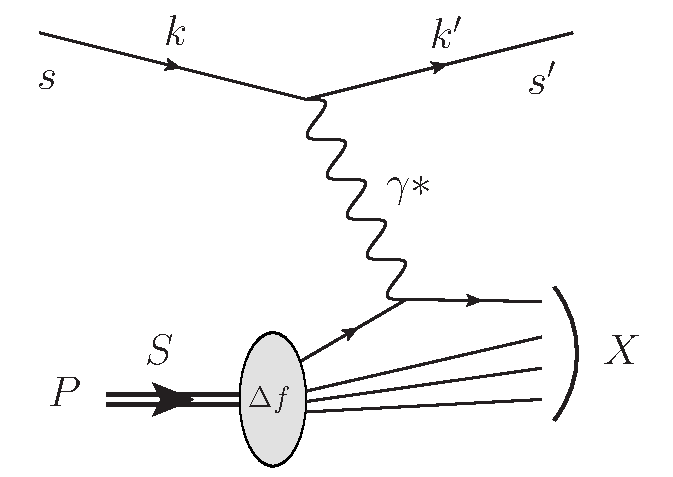
\includegraphics[width=0.5\textwidth]{DIS.pdf} 
  \caption{Feynman diagram for deep inelastic lepton-hadron scattering.}
  \label{fig:DIS_Feynamn}
\end{figure}
%%
The kinematics is worked out in the laboratory (LAB) reference frame, which corresponds to the fixed-target (FT) frame in polarised experiments\footnote{\footnotesize It must be observed that no polarised DIS experiments at colliders exist so far. Hence, in the polarised case the description can be limited to fixed-target experiments.}. The four-momenta are defined as follows
%%
\begin{equation}
    \begin{split}
        &k^{\mu} \;=\; \left(E, \vb{k} \right), \\
        &k'^{\mu} \;=\; \left(E', \vb{k'} \right), \\
        &P^{\mu} \;=\; \left(M, \vb{0} \right),
    \end{split}
\end{equation}
%%
where $M$ is the nucleon mass. I will make use of the following invariant variables
%%
\begin{align}
        & \nu = \frac{q \cdot P}{M} = E - E' \;\; \textrm{the energy lost by incoming lepton},
        \label{eq:nu}\\[5pt]
        & Q^2 = - q^2 \;\; \textrm{the virtuality of the exchanged photon},
        \label{eq:Q2}\\
        & x=\frac{Q^2}{2M\nu} \;\; \textrm{the Bjorken variable},
        \label{eq:x}\\
        & y = \frac{q\cdot P}{k \cdot P} = \frac{\nu}{E} \; \; \textrm{the energy fraction lost by the incoming lepton},
        \label{eq:y}\\
        & W^2 = \qty(P + q)^2 = M^2 + Q^2 \frac{1-x}{x} \;\; \textrm{the invariant mass of the system X}.
        \label{eq:W2}
\end{align}
%%
The process  is said to be "deep" when $Q^2 \gg M^2$ (\textit{i.e.} large momentum transfer), whereas the attribute "inelastic" is appropriate when $W^2 \gg M^2$ (\textit{i.e.} the hadron target is much inelastically excited). The amplitude for a process representing Fig.~\ref{fig:DIS_Feynamn}, with a generic final state $X$, is given by
%%
\begin{equation}
    \mathcal{M} = (-i e) \, \overline{u}(k',s') \, \gamma^{\mu}\, u(k,s) \, \frac{-i}{q^2} \, (-i e)\bra{X} j_{\mu}^{em} \qty(0) \ket{P,S} \,.
    \label{eq:ch2:amplitude}
\end{equation}
%%
Being a totally-inclusive process, no particular particles in the final state are detected. Hence, the total cross-section must take into account all the possible out-states, that is a sum over all the possible states $X$. For this reason, only two kinematic variables, among those listed in Eqs.~(\ref{eq:nu}-\ref{eq:W2}) are required to provide a complete description of the process. The differential cross-section for the process $2 \rightarrow 1 + n_X$ in the FT frame is given by 
%%
\begin{equation}
    d\sigma = \frac{1}{4 \qty|\vb{k}| M} \sum_{X} \qty| \mathcal{M} \qty( \ell N \rightarrow \ell'X ) |^2 \, \widetilde{d k'} \,  d\Phi_X \, ,
    \label{eq:ch2:dsigma}
\end{equation}
%%
where
%%
\begin{equation}
        d \Phi_X = \qty(2\pi)^4 \delta^{(4)} \qty( k + P - k' - P_X ) \widetilde{dP_X}  
\end{equation}
%%
and $\widetilde{dP_X}$ is the Lorentz invariant phase-space measure
%%
\begin{equation}
    \widetilde{d\, P_X} = \frac{d^3 \, P_X}{2 E_X (2\pi)^3} \,.
\end{equation}
%%
An identical definition holds also for $\widetilde{d k'}$.  Since the measurements in inclusive DIS concern only the final lepton $\ell'$, one can integrate over the entire momentum space in the hadron state and thus rewrite eq. \eqref{eq:ch2:dsigma} as
%%
\begin{equation}
    \begin{split}
        d\sigma &= \frac{1}{4 \qty|\vb{k}| M} \sum_{X} \int d\Phi_X \qty| \mathcal{M} \qty( \ell N \rightarrow \ell'X ) |^2 \widetilde{d k'}  \\
        & = \frac{1}{4 \qty|\vb{k}| M}  \frac{e^4}{q^4} \qty[ \overline{u}_{s'}(k') \, \gamma^{\mu}\, u_s(k)] \qty[\overline{u}_{s}(k) \,\gamma^{\nu}\, u_{s'}(k') ] \; \frac{d^3 \, k'}{2 E' (2\pi)^3} \times \\
        & \hspace{10mm} \sum_{X} \int d\Phi_X  \bra{X} j_{\mu}^{em} \qty(0) \ket{P,S} \; \bra{P,S} j_{\nu}^{em} \qty(0) \ket{X}  \\
        & = \frac{\alpha_{\textrm{em}}^2}{2 M \qty|\vb{k}| q^4} L_{\mu\nu} W^{\mu\nu} \qty|\vb{k}'| dE' d\Omega \,,
        \label{eq:ch2:dsigma2}
    \end{split}
\end{equation}
%%
where in the last equality I used $d^3 \, k' = \qty| \vb{k}' |^2 d|\vb{k}'| d\Omega$, and $d\Omega$ is the solid angle of the outgoing lepton in the LAB reference frame. The tensors $L_{\mu\nu}$ and $W_{\mu\nu}$ are defined as follows
%%
\begin{align}
    &L_{\mu\nu} = \qty[ \overline{u}_{s'}(k') \, \gamma^{\mu}\, u_s(k)] \qty[\overline{u}_{s}(k) \,\gamma^{\nu}\, u_{s'}(k') ] \,,
    \label{eq:ch2:lep_tens} \\
    &W_{\mu\nu} = \frac{1}{2\pi} \sumint_{X}  d\Phi_X  \bra{X} j_{\mu}^{em} (0) \ket{P,S}  \bra{P,S} j_{\nu}^{\dag em} (0) \ket{X}  \,,
    \label{eq:ch2:had_tens}
\end{align}
%%
where $\sumint_{X}$ is a shorthand notation to express the sum and the integral over the final state $X$. In the DIS limit, one can make use of the following approximations
%%
\begin{align}
    &k^2 = k'^2 \approx 0 \hspace{2mm} \Rightarrow \hspace{2mm} E \approx \qty| \vb{k} |, \hspace{2mm} E' \approx \qty| \vb{k'}|  \,,
    \label{eq:ch2:lep_approx}\\
    &Q^2 = - \qty(k - k')^2 \approx  2EE' \qty(1 - \cos \theta) = 4EE' \sin^2 \qty(\frac{\theta}{2}) \,,
    \label{eq:ch2:Q2_approx}
\end{align}
%%
where $\theta$ is the angle between the incoming and the scattered leptons. Inserting Eqs.~(\ref{eq:ch2:lep_approx},\ref{eq:ch2:Q2_approx}) in Eq.~\eqref{eq:ch2:dsigma2} one obtains 
%%
\begin{equation}
    \frac{d^2\,\sigma}{dE' \, d\Omega} = \frac{\alpha_{\textrm{em}}^2}{2MQ^4} \frac{E'}{E} L_{\mu\nu}W^{\mu\nu} = \frac{\alpha_{\textrm{em}}^2 E'}{s\, Q^4} L_{\mu\nu}W^{\mu\nu}\,,
    \label{eq:ch2:dsigma3}
\end{equation}
%%
where $s = (k + P)^2 \approx 2 M E$ is the Mandelstam variable. This expression gives the differential cross-section as a function of the energy of the outgoing lepton $E'$ and the scattered solid angle $\Omega$, both evaluated in the FT frame. It is possible to express Eq.~\eqref{eq:ch2:dsigma3} in terms of the Lorentz invariant dimensionless variables Eqs.~[\ref{eq:x}-\ref{eq:y}] by performing the transformation $(E', \theta) \rightarrow (x,y)$, which leads to
%%
\begin{equation}
    \frac{d^3 \, \sigma}{dx \, dy \, d\varphi} = \frac{\alpha_{\textrm{em}}^2 y}{2 Q^4} L_{\mu\nu} W^{\mu\nu} \,,
    \label{eq:ch2:dsigma4}
\end{equation}
%%
where $\varphi$ is the azimuthal angle of the scatted lepton. It is worth noting that, in computing Eq.~\eqref{eq:ch2:dsigma4}, the sum over the lepton and the hadron spin has not been taken into account. In principle, the lepton and hadron tensors can contain both symmetric and antisymmetric contributions. However, in the polarised case only the antisymmetric component survives, as I will show later.

%___________________________________________________________________________
\subsection*{Leptonic tensor}
The matrix element described by the lepton tensor can be decomposed into a symmetric and an antisymmetric part under $\mu \leftrightarrow \nu$ exchange. First, let us observe that the polarised spinor $u \qty(k, \, s)$, with polarisation vector $s$, satisfies the identity 
%%
\begin{equation}
    u \qty(k, \, s) \overline{u} \qty(k,\,s) = \frac{1}{2} (1 - \gamma_5 \slashed{s})  \qty(\slashed{p} + m)\,.
\end{equation}
%%
After summing over the spin of the scattered lepton $s'$, the lepton tensor can be written as a trace over gamma matrices
%%
\begin{equation}
    \begin{split}
        L_{\mu \nu} \qty(k,\,s;\, k') &= \frac{1}{2} \Trace \qty[ \qty(\slashed{k}' + m) \gamma_{\mu} \qty(1 - \gamma_5 \slashed{s}) \qty(\slashed{k} + m) \gamma_{\nu} ]\\
        & = \frac{1}{2} \Bigl\{ \Trace \qty[ \slashed{k} \gamma_{\mu} \slashed{k'} \gamma_{\nu} ] + m_{\ell} s^{\lambda} \Trace \qty[ \gamma_{\lambda} \gamma_{\nu} \gamma_{\rho} \gamma_{\mu} \gamma_{5} ] \qty( k - k' )^{\rho} \Bigr\}\\
        & = L_{\mu \nu}^{(S)} + i L_{\mu \nu}^{(A)} \,,
    \end{split}
\end{equation}
%%
where $L_{\mu \nu}^{(S)}$ and $L_{\mu \nu}^{(A)}$ are the symmetric and antisymmetric parts defined as 
%%
\begin{equation}
  L_{\mu \nu}^{(S)} \qty(k;\, k') = \frac{1}{2} \Trace \qty[ \slashed{k} \gamma_{\mu} \slashed{k'} \gamma_{\nu} ] = 2 \Bigl[k'_{\mu} k_{\nu} + k_{\mu} k_{\nu}' - g_{\mu \nu} \qty( k \cdot k' ) \Bigr]
\end{equation}
%%
\begin{equation}
  L_{\mu \nu}^{(A)} \qty(k,\,s;\, k') = \frac{1}{2i} m_{\ell} s^{\lambda} \Trace \qty[  \gamma_{\mu} \gamma_{\nu} \gamma_{\lambda} \gamma_{\rho} \gamma_{5} ] \qty( k - k' )^{\rho} = 2m_{\ell} \epsilon_{\mu \nu \lambda \rho } s^{\lambda} \qty( k - k' )^{\rho}\,.
\end{equation}
%%
If the momentum of the incoming lepton is aligned with the quantization axis, the spin vector can expressed as
%%
\begin{equation}
    s^{\mu} = \frac{\lambda_{\ell}}{m_{\ell}} k^{\mu}\, ,
    \label{eq:ch2:spin_vector}
\end{equation}
%%
where $\lambda_{\ell}$ is the helicity of the particle. It expresses whether the spin is parallel ($\lambda_{\ell} = +1/2$) or antiparallel ($\lambda_{\ell} = -1/2$) to the direction of motion of the particle. Thus, the antisymmetric component of the leptonic tensor can be finally expressed as
%%
\begin{equation}
    L_{\mu \nu}^{(A)} \qty(k,\,s;\, k') = 2\lambda_{\ell} \epsilon_{\mu \nu \lambda \rho} k^{\lambda} q^{\rho} \,,
    \label{eq:lep_tens_anti}
\end{equation}
%%
where the mass term $m_{\ell}$ has been cancelled by the denominator of Eq.~\eqref{eq:ch2:spin_vector}.

%________________________________
\subsection*{Hadronic tensor}
The hadronic tensor $W^{\mu \nu}$ encodes information on the proton structure. It receives non-perturbative contributions and, for that reason, its analysis cannot be addressed by a fully perturbative approach in QCD. However, exploiting symmetry constraints, the tensor can be decomposed into four scalar structure functions: the unpolarised functions $F_{1,2}$ and the helicity-dependent functions $g_{1,2}$, as long as parity violation is not concerned. Usually, these functions are measured by experiments and compared with theoretical predictions. These strongly depend on the theoretical model adopted to compute the observable, as I will show.%

In order to exploit symmetry constraints, I first rewrite the hadronic tensor as follows
%%
\begin{equation}
    \begin{split}
        W_{\mu\nu} &= \frac{1}{2\pi} \sumint_{\;\;X} \tilde{d P_X} \int d^4z \, e^{iz \cdot \qty(q + P - P_{X})}\bra{X} j_{\nu}(0) \ket{P,S} \bra{P,S} j^{\dag}_{\mu}(0) \ket{X}\\
        & = \frac{1}{2\pi} \sumint_{\;\;X} \tilde{d P_X} \int d^4z \, e^{iz \cdot q}\bra{X} j_{\nu}(0) \ket{P,S} \bra{P,S} j^{\dag}_{\mu}(z) \ket{X} \\
        & = \frac{1}{2\pi} \int d^4z \, e^{i z \cdot q} \bra{P,S} j^{\dag}_{\mu}(z) j_{\mu}(0) \ket{P,S} \,.
    \end{split}
    \label{eq:ch2:hadronic_tensor}
\end{equation}
%%
In the first line of Eq.~\eqref{eq:ch2:hadronic_tensor} the momentum-conservation delta function is expressed in its integral representation, introducing the dummy-variable z. The second line is the result of the transformation of the current-operator $j^{\dag}_{\mu}(0)$ by a space-time transformation 
%%
\begin{equation}
    \bra{P,S} j^{\dag}_{\mu}(0) \ket{X} =  \bra{P,S} e^{-i\hat{P}z} \, j^{\dag}_{\mu}(z) \, e^{i\hat{P}z} \ket{X} =  e^{-i z \cdot \qty(P - P_X )}\bra{P,S} j^{\dag}_{\mu}(z) \ket{X}\,.
\end{equation}
%%
Finally, the last line follows from the closure relation $\sumint_{\;\; X} \ket*{X} \bra*{X} = 1 $. In sanalogy with the lepton case, the hadronic tensor can be decomposed into a symmetric and an antisymmetric part
%%
\begin{equation}
    W_{\mu \nu} =  W_{\mu \nu} (q, \;P ) + i W_{\mu \nu} (q, \;P ; \; S ) \,.
\end{equation}
%%
Then, one can make the following observations:
\begin{enumerate}
    \item The hadronic tensor can be at most a function of $q, P$ and the spin vector of nucleon $S$, that is $W_{\mu \nu} = W_{\mu \nu}\qty(q,P;S)$.  
    \item The electromagnetic current must be conserved, that is $\partial \cdot j = 0$. In Eq.~\eqref{eq:ch2:hadronic_tensor}, this corresponds to the constraint $q_{\mu} W^{\mu \nu} = 0$.
    \item The hadronic tensor is hermitian, \textit{i.e.} $W_{\mu \nu} = \qty(W_{\mu \nu})^{*}$, as can be easily seen from eq. \eqref{eq:ch2:had_tens}. 
    \item The antisymmetric part of the hadroninc tensor is expected to change under reverse of the nucleon polarisation, hence the antisymmetric part must be linear in the polarisation vector.
    \item The strong interaction is parity invariant.
\end{enumerate}
Exploiting these constraints one finally obtains the most general form of the hadronic tensor \cite{collins_2011}
%%
\begin{equation}
  \begin{split}
  W_{\mu \nu}^{(S)} & = 2\qty(-g_{\mu \nu} + \frac{q_{\mu} q_{\nu}}{q^2}) F_1 \qty(x, Q^2) \\
  & + \frac{2 F_2 \qty(x , Q^2) }{P \cdot q} \qty(P_{\mu} - q_{\mu} \frac{P \cdot q}{q^2}) \qty(P_{\nu} - q_{\nu} \frac{P \cdot q}{q^2})\,,
  \label{eq:ch2:had_tens_final_symm}
  \end{split}
\end{equation}
%%
\begin{equation}
  \begin{split}
    W_{\mu \nu}^{(A)}  =  \epsilon_{\mu \nu \alpha \beta} \frac{q^{\alpha}2 M}{P \cdot q} \Biggl\{S^{\beta} g_1 \qty(x, Q^2) + \qty(S^{\beta} - P^{\beta} \frac{S \cdot q}{P \cdot q}) g_2 \qty(x,Q^2) \Biggr\} \,,
    \label{eq:ch2:had_tens_final_anti}
  \end{split}
\end{equation}
%%
The spin-independent coefficients $F_1,\, F_2$ and the spin-dependent ones $g_1,\,g_2$ are usually called \textit{structure functions} or \textit{form factors}. In the literature (see \textit{e.g.} Ref.~\cite{leader_2001,Anselmino:1994gn}), the hadronic tensor is also parametrised in terms of the fucntions $W_1 ,\, W_2$ and $G_1,\, G_2$, that are related with those in Eqs.[\ref{eq:ch2:had_tens_final_symm}-\ref{eq:ch2:had_tens_final_anti}] as follows:
%%
\begin{equation}
  F_1 (x, Q^2) = M W_1 (\nu, Q^2)\,, \hspace{5mm} F_2(x,Q^2) = \nu W_2 (\nu,Q^2)
\end{equation}
%%
\begin{equation}
  g_1 (x, Q^2) = M^2 \nu G_1 (\nu, Q^2) \,, \hspace{5mm} g_2 (x, Q^2) = M \nu^2 G_2 (\nu, Q^2)\,.
\end{equation}
%%
The symmetric and antisymmetric parts of the hadronic tensor can be recast as\footnote{\footnotesize The Particle Data Group (\href{https://pdg.lbl.gov/2019/reviews/rpp2019-rev-structure-functions.pdf}{PDG})~\cite{10.1093/ptep/ptaa104} reports the expressions of the hadronic tensor, Eqs.~(\ref{eq:ch2:had_tens_final_symm}-\ref{eq:ch2:had_tens_final_anti}), with the normalisation $S^2 = - M^2$ and $S \cdot P = 0$, whereas in this derivation I use $S^2 = - 1$.}
%%
\begin{equation}
  \begin{split}
    \frac{1}{2M} W_{\mu \nu}^{(S)} (q; \; P) & = \qty(-g_{\mu \nu} + \frac{q_{\mu} q_{\nu}}{q^2}) W_1( P \cdot q. \; q^2) \\
    & + \frac{W_2 (P\cdot q,\; q^2)}{M^2} \Biggl[ \qty(P_{\mu} - q_{\mu} \frac{P \cdot q}{q^2}) \qty(P_{\nu} - q_{\nu} \frac{P \cdot q}{q^2}) \biggr]
  \end{split}
  \label{eq:ch2:had_tens_symm}
\end{equation}
%%
\begin{equation}
  \begin{split}
    \frac{1}{2M} W_{\mu \nu}^{(A)} (q; \; P, \; S) & = \epsilon_{\mu \nu \alpha \beta} q^{\alpha} \Biggl\{ M S^{\beta} G_1 \qty(P\cdot q, Q^2) \Biggr.\\
    & +  \Biggl. \frac{G_2 \qty(P \cdot q,\;Q^2)}{M} \qty[ (P \cdot q) S^{\beta} - (S \cdot q) P^{\beta} ]\Biggr\} \,,
  \end{split}  
\end{equation}
%%
Is it worth noting that the above expressions describe the pure electromagnetic process mediated by a single virtual photon. The inclusion of both neutral- and charged-current at energies near (or higher) the weak boson masses introduces parity violating terms in the decomposition of the hadronic tensor. Hence, four additional scalar functions appear, usually called $F_3, \; g_3,\; g_4$ and $g_5$. The first one multiplies a term that is spin independent and also antisymmetric, whereas the other are multiplied by terms that are spin dependent and symmetric. Because of that, the correspondence by which the symmetric part, Eq.~\eqref{eq:ch2:had_tens_final_symm}, is spin independent and the antisymmetric one, Eq.~\eqref{eq:ch2:had_tens_final_anti}, is spin dependent no longer holds. The spin-dependent and -independent parts becomes a superposition of symmetric and antisymmetric contributions. The general decomposition for the hadronic tensor in DIS can be found \textit{e.g.} in Ref.~\cite{Anselmino:1993tc}.%

In present measurements, the momentum transfer values of the lepton beams do not exceed  $Q^2 \approx 100 \; GeV^2$. Hence, contributions from a weak boson exchange can be safely neglected. However, future measurements may surpass this threshold and the most general decomposition for the hadronic tensor will become necessary. For instance, this will be the case of the future Electron Ion Collider (EIC) (see \textit{e.g.} Ref.~\cite{Borsa:2020lsz}), whose operation is expected to start in the 2030's.\par

\subsection{Polarised cross-section asymmetries}
The insertion of the decompositions for both the leptonic and hadronic tensor into the differential cross-section Eq.~\eqref{eq:ch2:dsigma4} yields to 
%%
\begin{equation}
  \frac{d^3 \, \sigma^{s,S}}{dx \, dy \, d\varphi} = \frac{\alpha_{\textrm{em}}^2 y}{2 Q^4} \Bigl[ L^{(S)}_{\mu\nu} W^{\mu\nu(S)} - L^{(A)}_{\mu\nu} W^{\mu\nu(A)}  \Bigr]\,.
  \label{eq:cross_section}
\end{equation}
%%
In order to single out the spin dependent contribution (\textit{i.e.} the antisymmetric part) one usually takes the difference of cross-sections, Eq.~\eqref{eq:cross_section}, with opposite target spins 
%%
\begin{equation}
  \frac{d^3 \, \Delta \sigma^{s,S}}{dx \, dy \, d\varphi} \equiv \frac{d^3 \, \sigma^{s,+S}}{dx \, dy \, d\varphi} - \frac{d^3 \, \sigma^{s,-S}}{dx \, dy \, d\varphi} = - \frac{\alpha_{\textrm{em}}^2 y}{Q^4} \; L^{(A)}_{\mu\nu} W^{\mu\nu(A)} \;,
  \label{eq:diff_cs}
\end{equation}
%%
where the contributions with the opposite target spins in the helicity-dependent part sum together, given that they are linear in the target spin.%

In this Thesis, I only consider longitudinally polarised leptons with spin along $(\uparrow)$ or opposite $(\downarrow)$ the direction of motion, whereas the nucleon is at rest with polarisation along or opposite an \textit{arbitrary} direction $\vb*{S}$. Hence, in the target rest frame the nucleon spin four-vector can be parametrised as
%%
\begin{equation}
  S^{\mu} = (0, \; \sin \alpha \cos\beta, \; \sin \alpha \sin \beta, \; \cos \alpha) \;,
  \label{eq:par_S}
\end{equation}
%%
and, assuming the incoming lepton to be aligned to the $z$-axis, one can write
%%
\begin{equation}
  \begin{split}
    & k^{\mu} = E (1,\; 0,\; 0,\; 1)\;, \\
    & k'^{\mu} = E'( 1,\; \sin\theta \cos \varphi,\; \sin\theta \sin \varphi, \; \cos \theta )\,.
    \label{eq:par_k}
  \end{split}
\end{equation} 
%%
After some algebra, the product of the two antisymmetric tensors that appear in Eq.~\eqref{eq:diff_cs} looks like 
%%
\begin{equation}
  \begin{split}
    L^{\mu \nu (A)} W_{\mu \nu}^{(A)} & = - \frac{8}{\nu} \lambda_{l} \Biggl\{ g_1(x,Q^2) \Bigl[ (q \cdot k)(q \cdot S) - q^2 (k \cdot S) \Bigr] \Biggr. \\
    & +  \Biggl. g_2 (x, Q^2) q^2\Bigl[ (k \cdot S) - \frac{(q \cdot S) (k \cdot P)}{P \cdot q} \Bigr] \Biggr\}\,.
  \end{split}
\end{equation}
%%
The Lorentz products can be expressed in terms of the parametrisations Eqs.~(\ref{eq:par_S}-\ref{eq:par_k}) and the cross-section difference is
%%
\begin{equation}
  \begin{split}
    \frac{d \Delta \sigma^{s,S}}{dx dy d\varphi} & = \frac{4 \alpha_{\T{em}}^2 y}{Q^2} \Biggl\{ \cos \alpha \left[ g_1(x,Q^2) \left( \frac{E}{\nu} + \frac{E'}{\nu} \cos \theta \right) - g_2(x,Q^2) \frac{2 E E'}{\nu^2} (1 - \cos \theta) \right] \Biggr. \\
    & + \Biggl. \sin\alpha \sin\theta \cos\phi \left[ g_1(x,Q^2) \frac{E'}{\nu} + g_2(x,Q^2) \frac{2EE'}{\nu^2} \right] \Biggr\}\,,
  \end{split}
  \label{eq:delta_sigma_1}
\end{equation}
%%
where $\phi = \varphi - \beta$. The r.h.s. of Eq.~\eqref{eq:delta_sigma_1} is not written in terms of the invariant variables $x$ and $y$, as the differential cross-section in the r.h.s. would require. By making use of Eqs.~(\ref{eq:x}-\ref{eq:y}), one can obtain the final expression for the differential cross-section difference
%%
\begin{equation}
  \begin{split}
    \frac{d \Delta \sigma^{s,S}}{dx dy d\varphi} & = \frac{4 \alpha_{\T{em}}^2}{Q^2} \Biggl\{ \cos \alpha \left[ g_1(x,Q^2) \left( 2 - y - \frac{y^2 \gamma^2}{2} \right) - g_2(x,Q^2) y \gamma^2 \right] \Biggr.\\
    & + \sin \alpha \cos \phi \sqrt{1 - y - \frac{y^2 \gamma^2}{4}} \gamma \left( y g_1(x,Q^2) + 2 g_2(x,Q^2) \right) \Biggl. \Biggr\}\,,
  \end{split}
  \label{eq:cs_diff_fin_S}
\end{equation}
%%
where I have introduced the $\mathcal{O}(1/Q)$ quantity 
%%
\begin{equation}
  \gamma = \frac{2Mx}{Q} \,.
  \label{eq:gamma}
\end{equation}
%%
%The above expression relies on the assumption of longitudinally polarised leptons. Even though it would be possible to deal with transversely polarised leptons, this is phenomenologically impractical. In fact, with transversely polarised leptons, Eq.~\eqref{eq:ch2:spin_vector} would no longer hold, since a spin perpendicular to the direction of motion requires that
%%
%\begin{equation}
%  s = (0,\,\hat{\vb{s}})\,, \hspace{5mm} \hat{\vb{s}} \cdot \hat{\vb{k}} = 0 \,,
%\end{equation}
%%
%where $\hat{\vb{k}}$ is the unit vector representing the direction of motion of the incoming lepton. Hence, the factor $E/m_{\ell}$ coming from Eq.~\eqref{eq:ch2:spin_vector} no longer appears to cancel the factor $m_{\ell}/E$ that arises in the cross-section difference Eq.~\eqref{eq:ch2:dsigma4}, such that this one turns out to vanish in the large energy limit $m_{\ell}/E \rightarrow 0$.%

When talking about longitudinal or transverse polarisations, one must specify the reference axis against which the nucleon polarisation is defined. It is customary to define the nucleon polarisation with respect to the lepton beam axis. In that regard, \textit{longitudinal} (\textit{transverse}) indicates the directions parallel (orthogonal) to the lepton beam and will be represented by the symbols $\Uparrow,\, \Downarrow$, ($\Rightarrow, \, \Leftarrow$). In particular, for longitudinally polarised nucleons, one has $\alpha=0$ and the cross-section difference takes the form
%%
\begin{equation}
  \frac{d^3 \, \Delta \sigma}{dx \, dy \, d\varphi} = \frac{d^3 \, \sigma^{\uparrow, \Uparrow}}{dx \, dy \, d\varphi} - \frac{d^3 \, \sigma^{\uparrow, \Downarrow}}{dx \, dy \, d\varphi} = \frac{4 \alpha_{\T{em}}^2}{Q^2}  \left[ g_1(x,Q^2) \left( 2 - y - \frac{y^2 \gamma^2}{2} \right) - g_2(x,Q^2) y \gamma^2 \right] \,,
  \label{eq:cs_diff_l}
\end{equation}
%%
whereas for transversely polarised nucleons $\alpha=\pi/2$ and
%%
\begin{equation}
  \frac{d^3 \, \sigma^{\uparrow, \Rightarrow}}{dx \, dy \, d\varphi} - \frac{d^3 \, \sigma^{\uparrow, \Leftarrow}}{dx \, dy \, d\varphi} = \frac{4 \alpha_{\T{em}}^2}{Q^2} \gamma\sqrt{1 - y - \frac{y^2 \gamma^2}{4}}  \Bigl[ y g_1(x,Q^2) + 2 g_2(x,Q^2) \Bigr] \cos \phi\,.
  \label{eq:cs_diff_t}
\end{equation}
%%
In the Bjorken limit $Q \rightarrow \infty$, the transverse asymmetry, Eq.~\eqref{eq:cs_diff_t}, is suppressed by the factor $\gamma$. On the other hand, in Eq.~\eqref{eq:cs_diff_l} only the structure function $g_2$ is suppressed by the same factor, whereas $g_1$ is not. Given that measurements are taken with high $Q^2$, only the longitudinal asymmetry, Eq.~\eqref{eq:cs_diff_l}, is of phenomenological interest, since its leading contribution, the structure function $g_1$, survives in the Bjorken limit.

Finally, the unpolarised cross-section can be retrieved from Eq.~\eqref{eq:cross_section} by averaging over the spin of the incoming lepton $(s_{\ell})$ and of the nucleon $S$
%%
\begin{equation}
  \frac{d^3 \sigma}{dx dy d\varphi} = \frac{1}{2} \sum_{s_{\ell}} \frac{1}{2} \sum_{S} \frac{d^3 \sigma^{s_{\ell},S}}{dx dy d\varphi} = \frac{\alpha_{\T{em}}^2 y}{2 Q^4} L_{\mu \nu}^{(S)}W^{(S)\mu \nu}\,.
\end{equation}
%%
In the same way as the polarised case, the cross-section can be written in terms of the unpolarised structure functions $F_1$ and $F_2$. After integrating over the azimuthal angle $\varphi$, the expression for the cross-section reads
%%
\begin{equation}
  \frac{d^2 \sigma}{dx dy} = \frac{4 \pi \alpha_{\T{em}}^2}{xyQ^2} \left[ xy^2 F_1(x,Q^2) + (1-y + \frac{x^2y^2 M^2}{Q^2})F_{2}(x,Q^2)\right] \,,
  \label{eq:unp_cs}
\end{equation}
%%
where the contribution of order $M^2/Q^2$ that multiplies the structure function $F_2$ can be neglected in the Bjorken limit $M/Q \rightarrow 0$. In this limit, Eq.~\eqref{eq:unp_cs} can be written as\\
%%
\begin{equation}
  \frac{d^2 \sigma}{dx dy} = \frac{2 \pi \alpha_{\T{em}}^2}{xyQ^2} \left[ Y_{+} F_2(x,Q^2) - y^2 F_{L}(x,Q^2) \right]\,,
\end{equation} 
%%
where $Y_{+} = 1 + (1-y^2)$ and 
%%
\begin{equation}
  F_{L} = F_2 - 2xF_1 \,.
  \label{eq:Callan_Gross}
\end{equation}

%___________________________________________________________________________
\section{Phenomenology of DIS}
\label{sec:phenom_DIS}
As previously introduced, deeply inelastic processes with different spin configurations of the nucleon target make it possible to extract information on the structure functions $g_1$ and $g_2$. However, the cross-section difference is a combination of these two functions, whose separation is achieved by further approximate procedures. The phenomenological approach used hereafter will only focus on the polarised structure function $g_1$ since it is the one related to longitudinally polarised targets that are used in experiments. Further details on the structure function $g_2$, which accounts for transversely polarised targets, may be found in Refs.~\cites{leader_2001, Anselmino:1994gn,leader_predazzi_1996}.%

The quantity that is actually measured in experiments with longitudinally or transversely polarised nucleon targets is a cross-section asymmetry defined as
%%
\begin{equation}
  A_{\parallel} = \frac{d\sigma^{\uparrow \Uparrow} - d\sigma^{\uparrow \Downarrow}}{d\sigma^{\uparrow \Uparrow} + d\sigma^{\uparrow \Downarrow}} \,, \hspace{5mm}  A_{\perp} = \frac{d\sigma^{\uparrow \Rightarrow} - d\sigma^{\uparrow \Leftarrow}}{d\sigma^{\uparrow \Rightarrow} + d\sigma^{\uparrow \Leftarrow}} \,,
  \label{eq:asymmetry}
\end{equation}
%%
where $d\sigma$ is a shorthand notation for $d^3\sigma/dxdyd\varphi$ and the denominator is twice the unpolarised cross-section. The asymmetries are usually related, via the optical theorem, to the imaginary part of the amplitude for the forward (off-shell) photo-absorption cross-section asymmetries $A_1$ and $A_2$ according to
%% 
\begin{align}
  A_{\parallel} = D(A_1 + \eta A_2)\,, \hspace{5mm} A_{\perp} = d(A_2 - \zeta A_1)\,,
\end{align}
%%
where 
%%
\begin{equation}
  A_1 = \frac{\sigma_{1/2}^T - \sigma_{2/3}^T}{\sigma_{1/2}^T + \sigma_{2/3}^T} \,, \hspace{5mm} A_2 = \frac{\sigma_{1/2}^{TL}}{\sigma_{1/2}^T + \sigma_{2/3}^T}\,,
\end{equation}
%%
and the kinematic factors have been defined as 
%%
\begin{align}
  & \varepsilon = \frac{4(1-y) - \gamma^2 y^2}{2 y^2 + 4(1-y) + \gamma^2 y^2} \,,\\
  & \zeta = \frac{\gamma(1 - y/2)}{1 + \gamma^2y/2} \,,\\
  & \eta = \frac{\varepsilon y \gamma}{1 - \varepsilon(1 - y)} \,,\\
  & D = \frac{1 - (1 - y)\varepsilon }{1 + \varepsilon R (x,Q^2)} \,,\\
  & d = D \frac{\sqrt{1 - y - \gamma^2 y^2 /4}}{1 - y/2}\,,
\end{align}
%%
Here $\sigma_{1/2}^T$ and $\sigma_{3/2}^T$ represent the cross-sections for the forward virtual Compton scattering with a transversely polarised photon with total helicity of the photon-nucleon system equal to 1/2 and 2/3, respectively; $\sigma_{1/2}^{TL}$ represents the interference term between the longitudinal and transverse contributions to the photo-absorption cross-section (for more details, see Ref.~\cite{leader_predazzi_1996}). By inverting Eqs.~(\ref{eq:cs_diff_l},\ref{eq:cs_diff_t}) and using Eqs.~\eqref{eq:asymmetry} it is possible to express the structure functions in terms of $A_1$ and $A_2$ and obtain
%%
%\begin{align}
 % & g_1(x,Q^2) = \frac{F_1(x,Q^2)}{(1+\gamma^2)(1 + \eta \zeta)} \left[ (1 + \gamma \zeta) \frac{A_{\parallel}}{D} - (\eta - \gamma) \frac{A_{\perp}}{d} \right] \,, \\
 % & g_2(x,Q^2) = \frac{F_1 (x, Q^2)}{(1 + \gamma^2)(1 + \eta \zeta)} \left[ \left( \frac{\zeta}{\gamma} - 1 \right) \frac{A_{\parallel}}{D} + (\eta + \frac{1}{\gamma}) \frac{A_{\perp}}{d} \right] \,,
%\end{align}
%%
%%
\begin{align}
  & g_1(x,Q^2) = \frac{F_1 (x,Q^2)}{1 + \gamma^2} \left[ A_1(x,Q^2) + \gamma A_2 (x,Q^2) \right] \,,
  \label{eq:g1_A12}\\
  & g_2(x,Q^2) = \frac{F_1 (x,Q^2)}{1 + \gamma^2} \left[ \frac{A_2}{\gamma} - A_1 \right] \,.
\end{align}
%%
In principle, separate measurements of $A_{\parallel}$ and $A_{\perp}$ are necessary to provide a direct determination of the structure functions $g_1$ and $g_2$, but in practice the majority of the experiments are performed with longitudinally polarised targets, hence only measuring $A_{\parallel}$. From Eq.~\eqref{eq:g1_A12} it is easy to see that, up to corrections of order $\mathcal{O}(M/Q)$, $g_1$ is completely determined by $A_1$, leading to the approximation
%%
\begin{equation}
  A_1 \approx \frac{A_{\parallel}}{D} \approx \frac{g_1}{F_1} \,.
  \label{eq:A1}
\end{equation}
%%
On the other hand, $g_2$ is determined by $A_{\perp}$ or $A_2$, even though it enters the analysis only as negligible small corrections, unless $Q^2$ is very small. However, kinematic cuts can be applied to the data set used in the PDF determination, so that the small-$Q^2$ region can be safely excluded. As I will discuss later in \chapref{ch:4}, the present analysis makes use of such kinematics cuts, and the only relevant observable is Eq.~\eqref{eq:A1}.

%_______________________________________________________
\section{A look inside the hadronic tensor}

The hadronic tensor $W_{\mu \nu}$ introduced in the previous section contains information about the structure of the nucleon and describes the interaction between the virtual photon and the composite nucleon. It has been parametrised in terms of four structure functions which can be in principle measured in DIS experiments.%

Even though QCD is known to be \textit{asymptotically free}, the structure function does involve non-perturbative contributions, since the initial state (the nucleon) is not the fundamental degrees of freedom of the theory, but a bound state of quarks and gluons. Such a dependence is also present in the PM, even though it is introduced heuristically. I will show that the structure function $g_1$ can be expressed in terms of longitudinally polarised quark and gluon distributions. Moreover, it is possible to give a \textit{factorised} expression for the structure function $g_1$, which allows for the separation of a hard, perturbative and process dependent part from a low-energy, universal contribution. The former can be worked out by computing the diagrams in perturbative QCD, whereas the latter is given by the PDFs, which parametrise the inner structure of the proton.%

Before moving on the framework of QCD, in this section I will first make use of the PM which gives an intuitive description, though not exhaustive, of nucleon structure. If nothing else, it also provides the first historical approach to the puzzle of the nucleon structure. Then, the same results will be retrieved by the QCD at LO, while higher order corrections will improve the accuracy and also introduce other contributions (such as the gluon and the sea quarks) not considered in the PM.


\subsection{The hadronic tensor in the Naive Parton Model}
\label{subsec:PM_hadronic_tensor}
The Parton Model was initially formulated by Feynman \cite{PhysRevLett.23.1415} and formalized by Bjorken and Paschos \cite{PhysRev.185.1975} with the intention of providing a microscopic description of DIS before the advent of QCD. The idea relies on the infinite-momentum frame of reference for the proton, which coincides with the ceneter-of-mass frame in high-energy DIS experiments. When viewed from this frame, the proton results Lorentz-contracted into a thin shape in the direction of the motion, so that the incident lepton scatters instantaneously from the individual constituents. Moreover, time dilation implies that the last interaction of the constituents occurred far away in time, so that it is possible to neglect the interactions that bind the constituents into a hadron. Based on this picture, the parton model asserts that inclusive DIS can be approximated as an incoherent sum of lepton-constituent quark interactions. Furthermore, the incoming and outgoing partons can be considered as massless free particles, in so far the momentum transfer $Q$ is large. In the infinite-momentum frame the transversal momentum can be neglected, as it is of order $M^2/Q$ (see \textit{e.g.} Ref.~\cite{collins_2011}). Thus, partons are considered to carry only a fractional momentum $\xi$ of the parent nucleon.\par
Going into the details, the PM asserts that the cross-section can be computed as
%%
\begin{equation}
  \frac{d^2 \sigma}{dx dy} = \sum_{q} e_q^2 \int d\xi \;f_q (\xi) \frac{d \hat{\sigma}}{dy}\,,
  \label{eq:PM_CS}
\end{equation}
%%
where $d \hat{\sigma}$ is the parton level cross-section for the elementary QED process $\ell \; q \rightarrow \ell' \; q$ and $f_q$ is the PDF, that is the probability density distribution of finding a parton of type $q$ with nucleon momentum fraction $\xi$. For polarised cross-section asymmetries, one should write
%%
\begin{equation}
  \frac{d \sigma^{\uparrow \Uparrow}}{dx dy} - \frac{d \sigma^{\uparrow \Downarrow}}{dx dy} = \sum_{q} e_q^2 \int d\xi \; \Delta f_q (\xi) \left[ \frac{d \Delta \sigma^{\uparrow \uparrow}}{dy} - \frac{d \Delta \sigma^{\uparrow \downarrow}}{dy} \right]
  \label{eq:PM_fact}
\end{equation}
%%
where $d \sigma^{\lambda_{\ell} \, \lambda_{q}}$ is the elementary cross-section with helicity states of the incoming lepton, $\lambda_{\ell}$, and of he struck parton, $\lambda_{q}$. Here, I have also introduced the helicity-dependent, or polarised PDFs, $\Delta f_{q}$, defined as the momentum densities of partons with spin parallel or antiparallel to the longitudinally polarised parent nucleon:
%%
\begin{equation}
  \Delta f_{q} (\xi) = f_{q}^{\uparrow}(\xi) - f_{q}^{\downarrow}(\xi) \,.
\end{equation}
%%
The Eq.~\eqref{eq:PM_CS} also affects the expression for the hadronic tensor. Instead of a factor $1/s$ entering Eq.~\eqref{eq:ch2:dsigma3}, at the partonic level there is instead a factor $1/\xi s$, since the squared center-of-mass energy of the lepton-parton scattering is $(xP + q)^2 \approx 2 \xi \, P \cdot q$. Hence, the parton model expression for the antisymmetric part of the hadronic tensor is
%%
\begin{equation}
  W^{(A) \mu \nu}= \sum_{q} e_q^2\int \frac{d \xi}{\xi} \; \Delta f_{q} (\xi) \Delta \mathcal{C}^{\mu \nu}_{q} (x,q,s) \, \delta((p + q)^2) \,,
  \label{eq:had_tens_PM}
\end{equation}
%%
where the $\delta$-function has been introduced to account for the mass-shellness of the outgoing parton. 
In Eq.~\eqref{eq:had_tens_PM}, $\Delta \mathcal{C}^{\mu \nu}_{q}$ represents the matrix element of the photon-parton interaction that can be computed at the lowest order in Quantum Electrodynamics (QED):
%%
\begin{equation}
  \Delta \mathcal{C}_q^{\mu \nu} (x,q,s) = - 2 m_q \varepsilon_{\mu \nu \alpha \beta} s^{\alpha} q^{\beta}\,.
  \label{eq:DeltaC}
\end{equation}
%%
One may observe that the vertex of the interaction between the struck parton and the virtual photon has the same structure as the antisymmetric part of the leptonic tensor. For this reason, the matrix element Eq.~\eqref{eq:DeltaC} is similar to Eq.~\eqref{eq:lep_tens_anti}, apart from a minus sign. By defining the two projectors
%%
\begin{align}
  & P_3^{\mu \nu} = \frac{(P \cdot q)^2}{b M^2 (q \cdot S)} \left[ (q \cdot S) S_{\lambda} + q_{\lambda}  \right] P_{\eta} \varepsilon^{\mu \nu \lambda \eta} 
  \\
  & P_4^{\mu \nu} = \frac{1}{b} \left\{ \left[ \frac{(P\cdot q)^2}{M^2} + 2 (P \cdot q) x \right]S_{\lambda} + (q \cdot S)q_{\lambda} \right\} P_{\eta} \varepsilon^{\alpha \beta \lambda \eta}\,,
\end{align}
%%
with 
%%
\begin{equation}
  b = -4M \left[ \frac{(P\cdot q)^2}{M^2}  + 2 (P \cdot q) x - (q \cdot S)^2\right]\,,
\end{equation}
%%
One can extract the structure functions from the hadronic tensor Eqs.~(\ref{eq:ch2:had_tens_final_symm}-\ref{eq:ch2:had_tens_final_anti}) such that
%%
\begin{align}
  &P_3^{\mu \nu} W_{\mu \nu} = g_2\,, \\
  &P_4^{\mu \nu} W_{\mu \nu} = g_1 + g_2 \,.
\end{align}
%%
By taking a proper combination of the two projections, one obtains the important results
%%
\begin{align}
  &g_1(x) \hspace{1mm} = \hspace{1mm} \frac{1}{2} \sum_{q} e_q^2 \Delta f_{q} (x, S) \,,
  \label{eq:g1_PM}\\
  &g_2 (x) \hspace{1mm} = \hspace{1mm} 0\,.
  \label{eq:g2_PM}
\end{align}
%%
Alternatively, one can obtain these results by computing the partonic-level cross-sections appearing in Eq.~\eqref{eq:PM_fact} and obtain
%%
\begin{equation}
  \frac{d \Delta \sigma^{\uparrow \uparrow}}{dy} = \frac{4 \pi \alpha_{em}^2}{Q^2} \frac{1}{y} \,, \hspace{5mm} \frac{d \Delta \sigma^{\uparrow \downarrow}}{dy} = \frac{4 \pi \alpha_{em}^2}{Q^2} \frac{(1-y)^2}{y}\,,
\end{equation}
%%
such that when inserted into Eq.~\eqref{eq:PM_CS} lead to the expression
%%
\begin{equation}
  \frac{d \sigma^{\uparrow \Uparrow}}{dx dy} - \frac{d \sigma^{\uparrow \Downarrow}}{dx dy} = \frac{4 \pi \alpha_{em}^2}{Q^2} \left[ \sum_{q} e_q^2 \Delta f_{q}(x) (2-y)\right] \,,
\end{equation}
%%
When compared with Eq.~\eqref{eq:cs_diff_l}, provided that the latter is integrated over the azimuthal angle $\varphi$ and the terms $\mathcal{O}(\gamma^2)$ are neglected, one obtains the same results reported in Eqs.~[\ref{eq:g1_PM}-\ref{eq:g2_PM}].\par
If an exact $SU(3)_f$ flavour symmetry is assumed, only the quarks $u,d,$ and $s$ and the relative antiquarks contribute to the structure function $g_1$, that is
%%
\begin{equation}
  \begin{split}
    g_1(x) & = \frac{1}{2} \left[ \frac{4}{9} \left( \Delta u(x) + \Delta \bar{u}(x) \right) + \frac{1}{9} \left(  \Delta d (x) + \Delta \bar{b}(x)  \right) + \frac{1}{9}\left(  \Delta d (x) + \Delta \bar{b}(x)  \right) \right] \\
    & = \frac{1}{9} \left[ \frac{3}{4} \Delta T_3 (x) + \frac{1}{4} \Delta T_8 (x) + \Delta \Sigma (x)  \right] \,,
  \end{split}
  \label{eq:g1_NPM_ev}
\end{equation}
%%
In the second line, the structure function have been expressed in terms of linear combinations of quark densities with specific transformation properties under the symmetry group $SU(3)_{f}$, and they are
%%
\begin{align}
  & \Delta \Sigma (x) = \Delta u^{+} (x) + \Delta d^{+} (x) +\Delta s^{+} (x) \,, \\
  & \Delta T_3 (x) = \Delta u^{+} (x) - \Delta d^{+} (x) \,, \\
  & \Delta T_8 (x) = \Delta u^{+} (x) + \Delta d^{+} (x) - 2 \Delta s^{+} (x) \,,
\end{align}
%%
where I have defined\\
%%
\begin{equation}
 \Delta q^{\pm}(x) = \Delta q(x) \pm \Delta \bar{q}(x) \,.
\end{equation}
%%
Under the same $SU(3)_f$ symmetry group, the linear combinations $\Delta \Sigma, \,\Delta T_3$ and $\Delta T_8$ transform as a flavour singlet, the third component of an isospin triplet, and the eight component of an $SU(3)_f$ octet, respectively.
%The results of the PM have been obtained in a sort of heuristic fashion, based on some intuitive, though powerful, assumptions. However, it is relevant to mention that a justification for such a picture can be given in the so-called \textit{impulse approximation}, when the intrinsic Fermi motion of quarks is neglected (see \textit{e.g.} Chap. 16.9 of Ref.~\cite{leader_predazzi_1996}). Using this approach, one can also allows for a transverse momentum of the partons, that is 
%%
%\begin{equation}
%  p^{\mu} \hspace{3mm}  = \hspace{3mm} \left( E_1, p_x, p_y, \xi P_{z} \right)\,.
%\end{equation}
%%
%In doing so, the structure function $g_2$ assumes a non-zero value. Still, the PM framework is not able to give an unambiguous prescription to calculate $g_2$, providing different results that are generally incompatible with each other. One reason for that is that the structure function $g_2$ is extremely sensitive to the difference between the masses $m_q$ of the approximatively free quarks if compared with that of the bound quark $m$. In the special case of longitudinal polarisation, this difference does not make any relevant alteration in the analysis, yielding the results shown in Eqs.~[\ref{eq:g1_PM}-\ref{eq:g2_PM}]. However, this is no longer true when the transverse spin is relevant, motivating the high sensitivity on the mass difference for $g_2$. Furthermore, if one sets $m \neq m_{q}$, the expression for the antisymmetric part of the hadronic tensor is not gauge invariant ($q^{\mu} W_{\mu \nu}^{(A)} \neq 0$). The gauge invariance is restored when only a field theoretic approach is adopted \cite{Anselmino:1993tc}.\par

\subsection*{Sum rules and spin crisis}
An important tool that can be used in parton determination are the moments structure functions, since they can be related to measurable quantities like the total momentum fraction carried by quarks or the total contribution of quark spin to the spin of the nucleon. Moreover, the Wilson Operator Product Expansion (OPE) can be applied to the Fourier transform of the nucleon matrix element of the electromagnetic current that appears in the hadronic tensor $W^{\mu \nu}$, Eq.~\eqref{eq:ch2:hadronic_tensor}. This affects the functional form of the moments of the structure functions. In fact, if the fields that enter the electromagnetic current are treated as free fields (\textit{i.e.} one adopts the PM picture), the first moment of the structure function $g_1$ can be expressed as\footnote{\footnote If the hypothesis of free fields is not assumed, then the coefficients that multiply the $a_i$ receive $Q^2$-dependent corrections that are calculable in perturbative QCD. However, their consideration does not affect the present discussion.}
%%
\begin{equation}
  \Gamma_{1}^{p} = \int_{0}^{1} dx \, g_{1}^{p}(x) = \frac{1}{12} \left\{ a_3 + \frac{1}{\sqrt{3}} a_8 + \frac{4}{3} a_{0} \right\}\,,
  \label{eq:g1_m1}
\end{equation}
%%
where the $a_i$ are hadronic matrix elements of the axial-vector currents $J^{i}_{5 \mu}$ ($i=1,\dots,8$) of the octet of $SU(3)_{f}$ and of the flavour singlet axial current $J^{0}_{5 \mu}$, taken between proton states of definite momentum and spin. It can be shown (see \textit{e.g.} Ref.~\cite{Anselmino:1993tc} and references therein) that $a_{3,8}$ are related to the two constants, $F$ and $D$, measured in the hyperon $\beta$-decay
%% 
\begin{align}
  & a_3 = F + D \,, \\
  & a_8 = \frac{1}{\sqrt{3}} (3F - D)\,.
\end{align}
%%
Hence, measurements of $\Gamma_{1}^{p}$ provide an estimation of the matrix element $a_0$ by simply inverting Eq.~\eqref{eq:g1_m1}
%%
\begin{equation}
  a_0 =  \frac{3}{4} \left\{ 12 \Gamma_{1}^p - a_3 - \frac{1}{\sqrt{3}} a_8 \right\}\,.
\end{equation}
%%
These relations become relevant when, in the framework of the naive PM, the hadronic matrix elements are expressed in terms of the polarised parton distributions~\cite{Anselmino:1993tc}, providing
%%
\begin{align}
  & a_0 \equiv \Delta \Sigma = \int_{0}^{1} dx \, \Delta \Sigma(x) \,, 
  \label{eq:a0_NPM}
  \\
  & a_3 = \int_{0}^{1} dx \, \left[ \Delta u^{+}(x) - \Delta d^{+}(x) \right] \,,
  \label{eq:a3_PM}
  \\
  & a_8 = \frac{1}{\sqrt{3}}\int_{0}^{1} dx \, \left[ \Delta u^{+}(x) + \Delta d^{+}(x) - 2 \Delta s^{+}(x) \right] \,.
  \label{eq:a8_PM}
\end{align}
%%
It is worth remarking that the results I have just obtained, Eqs.~(\ref{eq:a0_NPM}-\ref{eq:a8_PM}), rely on the assumption of exact $SU(3)_f$ flavour symmetry and on the conservation of the related currents. By looking at the physical significance of $\Delta \Sigma (x)$, it follows that
%%
\begin{equation}
  a_0 = \Delta \Sigma \equiv 2 \left< S_{z}^{\T{quarks} + \T{antiquarks}} \right> \,.
  \label{eq:a0_Sz}
\end{equation}
%%
Since the transverse parton momentum is zero, the orbital angular momentum carried by the quarks is perpendicular to $\vb*{P}$ and does not contribute to $J_{z}$. In addition, the polarisation of the gluons was not taken into account initially. Hence, the PM expectation for a proton with helicity $1/2$ was 
%%
\begin{equation}
  \left< S_{z}^{\T{quarks} + \T{antiquarks}} \right> = J_{z} = \frac{1}{2}
  \label{eq:J_z_NPM}
\end{equation}
%%
In the 80's the EMC collaboration measured the total contribution of quarks and antiquarks to the spin of the proton \cite{EuropeanMuon:1989yki} using Eq.~\eqref{eq:a0_Sz}. Surprisingly, instead of the expected result Eq.~\eqref{eq:J_z_NPM}, they obtaiend
%%
\begin{equation}
  \left< S_{z}^{\T{quarks} + \T{antiquarks}} \right> = 0.03 \pm 0.06 \pm 0.09 \,,
  \label{eq:EMC_exp}
\end{equation}
%% 
opening the "spin crisis" in the Parton Model \cite{Leader_Anselmino}. However, as pointed in Ref.~\cite{Leader:2016sli}, the  crisis was nothing but a consequence of the lack of understanding in the theory of strong interactions. 

%___________________________________________________________________________
\subsection{The Field Theoretic Model}
\label{sec:field_theoretic}

The heuristic approach paved the ground for the development of QCD. However, the calculations did not lead to coherent predictions when compared to experimental data, as I have just discussed. The adoption of QCD as the theory of strong interaction provides a more accurate description of the experimental results. Moreover, the accuracy increases with increasing perturbative order of the Feynman diagrams. At Born level the interaction is represented by the tree-level scattering of a quark (or antiquark) off the virtual photon $\gamma^{*}$. This coincides with the PM expectation. At higher order, QCD introduces several new contributions, which can be computed perturbatively. For instance, at $\mathcal{O}(\alpha_{s})$, the Feynman diagrams include the emission of a gluon, the one-loop corrections, and the process initiated by a gluon which then splits into a quark-antiquark pair, the so-called photon-gluon fusion process. In general, QCD interactions affect the predictions by two main features
\begin{enumerate}
  \item They introduce a perturbative calculable logarithmic $Q^2$ dependence in the parton densities.
  \item QCD naturally introduces the polarised gluon contribution to $g_1$.  
\end{enumerate}
These two effects are now discussed.

%% Field theoretic DIS figure
\begin{figure}[t]
  \centering
  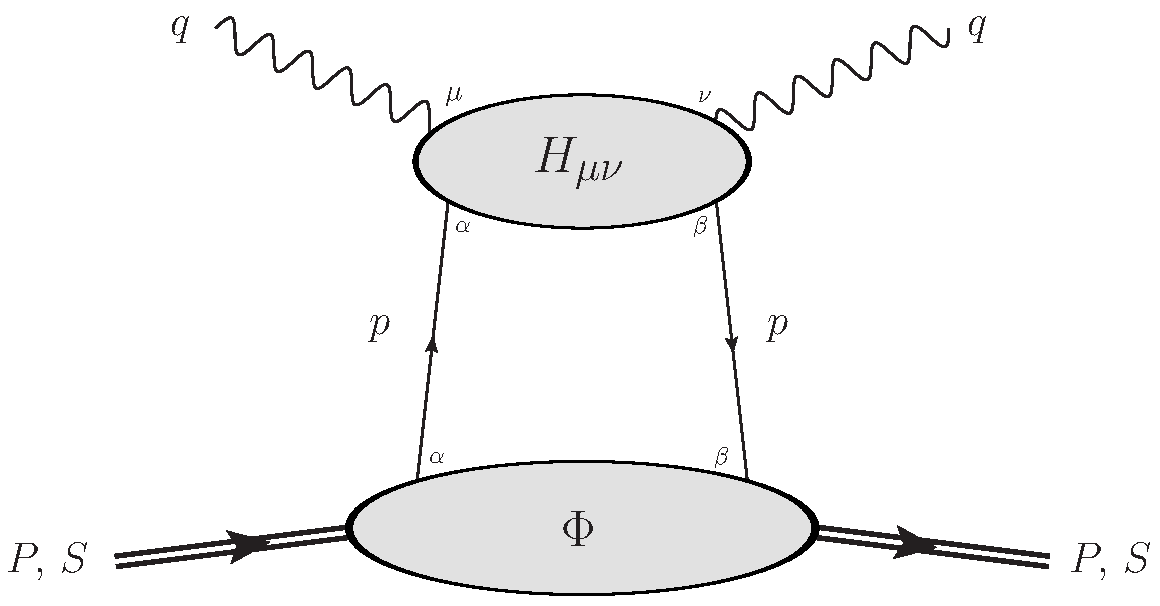
\includegraphics[width=0.5\textwidth]{DIS_FT.pdf} 
  \caption{Handbag diagram for DIS in the field theoretic model.}
  \label{fig:DIS_FT}
\end{figure}
%%

\subsubsection*{Perturbative corrections and the evolution equation}
The inclusion of gluonic corrections to the Born level introduces divergent contributions. These divergent terms arise from the so-called \textit{mass} or \textit{collinear} singularities that occur because of the effective masslessness of the quarks and are removed by the \textit{factorisation} process. The \textit{factorisation theorem} for DIS~\cite{Collins:1989gx} allows for a separation of the interaction into a 'hard' perturbative part $H^{\mu \nu}_{\alpha \beta}$ (the top 'blob') and a 'soft' non-perturbative part $\Phi_{\alpha \beta}$, represented by the "top" and "bottom" blobs of Fig.~\ref{fig:DIS_FT}, respectively. Schematically, the computation of the hard part gives origin to terms of the form $\alpha_{s} \ln Q^2/m_q^2$, which are split as follows
%-------------------------------
\footnote{Here the divergent contribution is given by the mass term inside the logarithm. However, this term arises only when the computation of the hard part is worked out keeping a non-vanishing mass for the quark. Otherwise, the singularity arises as an infrared logarithmic divergence of the type $\alpha_{s} \ln Q^2/\mathcal{K}^2$, where $\mathcal{K}$ is the cut-off in momentum space.}
%-------------------------------
%%
\begin{equation}
  \alpha_{s} \ln \frac{Q^2}{m_q^2} = \alpha_{s} \ln \frac{Q^2}{\mu^2} + \alpha_{s} \ln \frac{\mu^2}{m_{q}} \,.
\end{equation}
%%
The first term on the r.h.s. is absorbed into the hard part, whereas the other one is absorbed into the soft part (\textit{i.e.} the PDF), which in any case has to be parametrized and studied experimentally. This procedure introduces a \textit{factorisation scale} $\mu^2$, that is the scale at which the separation is made. As a consequence, PDFs acquire a dependence on the scale of the process, whereas the remaining finite part incorporates $Q^2$-dependent terms which correct the expression for the structure functions, thus breaking Bjorken scaling.%

If all orders in perturbation theory were considered, the physical observables would not depend on this scale, thus making the choice of its value completely arbitrary. However, it turns out that predictions are truncated at some fixed order in perturbation theory, and the choice of the values does make some difference. Usually, the optimal choice is $\mu^2 = Q^2$, so that the PDFs will now depend on $x$ and $Q^2$
%%
\begin{equation}
  \Delta f(x)  \hspace{2mm} \longrightarrow \hspace{2mm} \Delta f(x,Q^2) \,.
  \label{eq:Q2_pdf}
\end{equation}
%%
If one keeps only the leading logarithmic (LL) terms proportional to $\alpha_{s} \ln Q^2/\mu^2$, one recovers the PM expressions for the polarised structure functions, Eq.~\eqref{eq:g1_PM}, provided the replacement reported in \eqref{eq:Q2_pdf}.\par
The variation with $Q^2$ is controlled by the Dokshitzer, Gribov, Lipatov, Altarelli and Parisi (DGLAP) evolution equations \cite{Altarelli:1977zs, Dokshitzer:1977sg, Gribov:1972ri}, a set of $(2 n_f + 1)$ coupled integro-differential equations. For the polarised densities, these equations read
%%
%\begin{equation}
%  \begin{split}
%    \frac{\partial}{\partial \ln Q^2} \Delta q_{i} (x,Q^2) = \frac{\alpha_{s}(Q^2)}{4 \pi} \int_{x}^{1} \frac{dy}{y} &\left\{\sum_{k}^{n_f} \left[ \Delta P_{q_i q_k} \left( \frac{x}{y} \right) \Delta q_k(y,Q^2) + \Delta P_{q_i \bar{q}_k} \left(\frac{x}{y}\right) \Delta \bar{q}_k(y,Q^2) \right]\right. \\
%    & \left. + \Delta P_{q_i g} \left(\frac{x}{y}\right) \Delta g (y, Q^2) \right\}
%  \end{split}
%\end{equation}
%%
%\begin{equation}
%  \begin{split}
%    \frac{\partial}{\partial \ln Q^2} \Delta g_{i} (x,Q^2) = \frac{\alpha_{s}(Q^2)}{4 \pi} \int_{x}^{1} \frac{dy}{y} &\left\{\sum_{k=1}^{n_f} \left[ \Delta P_{g q_k} \left( \frac{x}{y} \right) \Delta q_k(y,Q^2) + \Delta P_{g \bar{q}_k} \left(\frac{x}{y}\right) \Delta \bar{q}_k(y,Q^2) \right]\right. \\
%    & \left. + \Delta P_{g g} \left(\frac{x}{y}\right) \Delta g (y, Q^2) \right\}
%  \end{split}
%\end{equation}
%%
\begin{equation}
  \frac{\partial}{\partial \ln Q^2} 
  \left(\begin{matrix}
    \Delta q_i \\
    \Delta g \\
    \Delta \bar{q}_i
  \end{matrix} \right) (x,Q^2) = \frac{\alpha_{s}(Q^2)}{4 \pi}  \sum_{k,l}
  \left(\begin{matrix}
    \Delta P_{q_i q_k} && \Delta P_{q_i g} && \Delta P_{q_i \bar{q}_l} \\
    \Delta P_{g q_k} && \Delta P_{g g} && \Delta P_{g \bar{q}_l} \\
    \Delta P_{\bar{q}_i q_k} && \Delta P_{\bar{q}_i g} && \Delta P_{\bar{q}_i \bar{q}_l} \\
  \end{matrix}\right) \otimes 
  \left(\begin{matrix}
    \Delta q_i \\
    \Delta g \\
    \Delta \bar{q}_i
  \end{matrix} \right) (x,Q^2) \,,
  \label{eq:DGLAP_coupled}
\end{equation}
%%
where $k,l$ run over the quark flavours ($k,l = u,\, d\, s,\, \dots$) and $\otimes$ is the shorthand notation for the convolution product with respect to x
%%
\begin{equation}
  f \otimes g = \int_{x}^{1} \frac{dy}{y} f \left(\frac{x}{y} \right) g(y) \,.
  \label{eq:def_conv}
\end{equation}
%%
The $\Delta P$ are the polarised \textit{splitting functions} and can be expanded in powers of the strong coupling $\alpha_s$
%%
\begin{equation}
  \Delta P = \sum_{n=0}^{\infty} \left( \frac{\alpha_s}{4\pi} \right)^{n} \Delta P^{(n)}(x)\,.
\end{equation}
%%
The evolution equations can be maximally decoupled from each other if one exploits charge conjugation invariance and $SU(n_f)$ flavour symmetry, which impose 
%%
\begin{equation}
  \begin{split}
    & \Delta P_{q_i q_j} = \Delta P_{\bar{q}_i \bar{q}_j} = \delta_{ij} P_{qq}^{V} + P_{qq}^{S} \,,\\
    & \Delta P_{\bar{q}_i q_j} = \Delta P_{q_i \bar{q}_j} = \delta_{ij} P_{\bar{q}q}^{V} + P_{\bar{q}q}^{S} \,,\\
    & \Delta P_{q_i g} = \Delta P_{\bar{q}_i g} = \Delta P_{qg} \,, \\
    & \Delta P_{g q_i} = \Delta P_{g \bar{q}_i} = \Delta P_{gq}
  \end{split}
\end{equation}
%%
Inserting these relations into Eq.~\eqref{eq:DGLAP_coupled} and using $\Delta q_{i}^{\pm} = \Delta q_{i} \pm \Delta \bar{q}_{i}$,
the evolution equations read 
%%
\begin{equation}
  \begin{split}
    \frac{\partial}{\partial \ln Q^2} 
    \left(\begin{matrix}
      \Delta q_i^{+} \\
      \Delta g \\
      \Delta \bar{q}_i^{-}
    \end{matrix} \right) & = \frac{\alpha_{s}(Q^2)}{4 \pi} 
    \left(\begin{matrix}
      (\Delta P_{qq}^{V} + \Delta P_{q\bar{q}}^{V}) && 2 \Delta P_{qg} && 0 \\
      \Delta P_{gq} && \Delta P_{gg} && 0 \\
      0 && 0 && (\Delta P_{qq}^{V} - \Delta P_{q\bar{q}}^{V})
    \end{matrix} \right) \otimes
    \left(\begin{matrix}
      \Delta q_i^{+} \\
      \Delta g \\
      \Delta \bar{q}_i^{-}
    \end{matrix} \right) 
    \\[10pt]
    & + \frac{\alpha_{s}(Q^2)}{4 \pi}
    \left(\begin{matrix}
      (\Delta P_{qq}^{S} + \Delta P_{q \bar{q}}^{S}) && 0 && 0 \\
      0 && 0 && 0 \\
      0 && 0 && (\Delta P_{qq}^{S} - \Delta P_{q\bar{q}}^{S})
    \end{matrix} \right) 
    \otimes
    \left(\begin{matrix}
      \sum_{k} \Delta q_k^{+} \\
      \Delta g \\
      \sum_{k} \Delta \bar{q}_k^{-}
    \end{matrix} \right)
  \end{split}
\end{equation}
%%
where the dependence on the kinematic has been momentarily omitted. Now the equations are semi-diagonalised, being the third equation completely decoupled from the rest of the system. It is convenient to express the system using the following definitions
%%
\begin{equation}
  \begin{split}
     \Delta \Sigma \equiv \sum_{k=1}^{n_{f}} \Delta q_{k}^{+}  \hspace{10mm} & \T{singlet distribution}\, ,\\
     \Delta V \equiv \sum_{k=1}^{n_{f}} \Delta q_{k}^{-}  \hspace{10mm} & \T{valence distribution}\,, \\
     \Delta q_{NS,is}^{\pm} \equiv \Delta q_{i}^{\pm} - \Delta q_{j}^{\pm} \hspace{10mm} & \T{non-singlet distribution} \,,
  \end{split}
  \label{eq:evb_dist}
\end{equation}
%%
for the polarised parton distributions and
%%
\begin{equation}
  \begin{split}
    & \Delta P^{\pm} \equiv \Delta P_{qq}^{V} \pm \Delta P_{q \bar{q}}^{V} \,,\\
    & \Delta P_{qq} \equiv \Delta P^{+} + n_{f} (\Delta P_{qq}^{S} + \Delta P_{q\bar{q}}^{S} )  \,,\\
    & \Delta P^{V} \equiv \Delta P^{-} + n_{f} (\Delta P_{qq}^{S} - \Delta P_{q \bar{q}}^{S}) \,,
  \end{split}
\end{equation}
%%
for the polarised splitting functions. Hence, the evolution equation can be expressed as follows
%%
\begin{equation}
  \begin{split}
    & \frac{\partial}{\partial Q^2} \Delta g  = \frac{\alpha_{s}(Q^2)}{4 \pi} \Bigl[ \Delta P_{gg} \otimes g + \Delta P_{gq} \otimes \Delta \Sigma \Bigr] \,,\\
    & \frac{\partial}{\partial Q^2} \Delta q^{+}_{i} = \frac{\alpha_{s}(Q^2)}{4 \pi} \Bigl[ \Delta P^{+} \otimes \Delta q_{i}^{+} + \frac{1}{n_f} (\Delta P_{qq} - \Delta P^{+}) \otimes \Delta \Sigma + 2 \Delta P_{qg} \otimes \Delta g \Bigr] \,,\\
    & \frac{\partial}{\partial Q^2} \Delta q^{-}_{i} = \frac{\alpha_{s}(Q^2)}{4 \pi} \Bigl[ \Delta P^{-} \otimes \Delta q_{i}^{-} + \frac{1}{n_f} (\Delta P^{V} - \Delta P^{-}) \otimes \Delta V \Bigr] \,,\\
  \end{split}
  \label{eq:evb_1}
\end{equation}
%%
At this point, it is customary to define the so-called \textit{evolution basis}, a specific set of linear combinations of distributions that maximally decouple the evolution equations. In particular, by looking at the Eqs.~\eqref{eq:evb_1} and using the definitions in Eqs.~\eqref{eq:evb_dist}, it is straightforward to verify that the evolution equations completely decouple for the non-singlet and valence distributions
%%
\begin{equation}
  \begin{split}
    & \frac{\partial}{\partial \ln Q^2}\Delta q_{\T{NS}ij}^{\pm} (x,Q^2) = \frac{\alpha_s(Q^2)}{4\pi} \Delta P^{\pm} \otimes \Delta q_{{\T{NS}ij}}^{\pm} (x,Q^2) \,, \\
    & \frac{\partial}{\partial \ln Q^2}\Delta V (x,Q^2) = \frac{\alpha_s(Q^2)}{4\pi} \Delta P^{V} \otimes \Delta V (x,Q^2)\,,
  \end{split}
\end{equation}
%% 
whereas the singlet and the gluon distributions remain coupled 
%%
\begin{equation}
  \frac{\partial}{\partial \ln Q^2} 
  \left(\begin{matrix}
    \Delta g (x,Q^2)\\
    \Delta \Sigma (x,Q^2)
  \end{matrix} \right) 
  = \frac{\alpha_{s}(Q^2)}{4 \pi} \otimes
  \left(\begin{matrix}
    \Delta P_{gg} && \Delta P_{gq} \\
    \Delta P_{qq} && \Delta 2n_f P_{qg}
  \end{matrix} \right)
  \otimes 
  \left(\begin{matrix}
    \Delta g (x,Q^2) \\
    \Delta \Sigma (x,Q^2)
  \end{matrix} \right) \,.
\end{equation}
%%
The dependence on the kinematics $(x,Q^2)$ have been restored.%

The polarised splitting functions have been computed at LO in Ref.~\cite{Altarelli:1977zs}, then extended at NLO in Ref.~\cite{Mertig:1995ny, Vogelsang:1995vh}; only recently splitting functions have been computed at NNLO in Ref.~\cite{Moch:2014sna}.%

Finally, a little complementary observation about the factorisation theorem. In principle, there could be several contributions to the process in the field theoretic approach. The factorisation theorem only refers to Fig.~\ref{fig:DIS_FT}, which represents the leading region for DIS when the light-cone gauge, $A^{+}=0$, is adopted. All the contributions coming from this diagram are called 'leading twist'. All the diagrams other than that shown in Fig.~\ref{fig:DIS_FT} have an overall suppression of order $(1/Q)^{n}$ and provide the so-called 'higher twist' corrections. Therefore, the complete expression for observables like structure functions should read
%%
\begin{equation}
  F(x, Q^2) = F(x, Q^2)^{LT} + \frac{F^{(1)}(x,Q^2)}{Q^2} + \dots \,.
\end{equation}
%%
There are two types of twist corrections -- target mass corrections, which are purely kinematical, and dynamical corrections. Regardless the origin of these contributions, they can be neglected by means of kinematic cuts applied to the data set, so that the small-$Q^2$ region is excluded. Kinematic cuts will be further discussed in Chap.~\ref{ch:4}, where the data sets will be presented.

\subsubsection*{The gluon contribution to $g_1$}
Another important consequence of the QCD analysis is the rise of the contribution from polarised gluons to the structure function $g_1$. Indeed, the leading-twist expression becomes 
%%
\begin{equation}
  g_1(x,Q^2) = \frac{1}{2} \sum_{i=1}^{n_f} e_{q}^2 \Biggl\{ \Delta \mathcal{C}_{q} \otimes \Bigl[ \Delta q_i (x,Q^2) + \Delta \bar{q}_i (x,Q^2) \Bigr] + \Delta \mathcal{C}_{g} \otimes \Delta g (x,Q^2)\Biggr\} \,,
  \label{eq:g1_QFT}
\end{equation}
%%
where the gluon contribution is defined as
%%
\begin{equation}
  \Delta g(x,Q^2) = g^{\uparrow}(x,Q^2) - g^{\downarrow}(x,Q^2) \,.
\end{equation}
%%
In Eq.~\eqref{eq:g1_QFT}, the sum runs over the flavours of quarks and antiquarks, $\otimes$ denotes the usual convolution in Eq.~\eqref{eq:def_conv}, and finally $\Delta \mathcal{C}_{q}$ and $\Delta \mathcal{C}_{g}$ are the \textit{coefficient functions} which are related to the hard photon-quark or photon-gluon cross-sections. Coefficient functions are perturbative quantities and can be expanded in a power series of $\alpha_s$
%%
\begin{equation}
  \Delta \mathcal{C} \left( y, \alpha_s \right) = \Delta \mathcal{C}^{(0)}_{p} (y) + \frac{\alpha_s}{4\pi} \Delta \mathcal{C}^{(1)}_{p} (y) + \mathcal{O}(\alpha_s^2)\,,
\end{equation}
%% 
where $p=q,g$ and
%%
\begin{equation}
  \left\{ \hspace{-3mm}
  \begin{array}{cl}
    &\Delta \mathcal{C}_{q}^{(0)} (y) = \delta(1-y)\,,\\[10pt]
    &\Delta \mathcal{C}_{g}^{(0)} (y) = 0 \,.\\
  \end{array}
  \right.
\end{equation}
%%
At the lowest order, the gluon distribution does not contribute to the structure function, hence the Naive Parton Model expectation, Eq.~\eqref{eq:g1_PM}, is recovered. At higher orders, the simple and intuitive picture provided by the PM no longer holds, and the Bjorken variable $x$ loses its interpretation as fractional momentum.\par
Now that I have introduced the polarised gluon distribution, it is possible to revise the unexpected result, Eq.~\eqref{eq:EMC_exp}. In the PM, the axial current $a_0$ can be regarded as the spin quark operator, since it is related to the first moment of the singlet quark distribution. The key point is that the axial current $a_0$ is conserved only in a massless and \textit{free-field} theory. However, when one allows for interactions among quarks, the current is no longer conserved, even when the masses of partons are neglected. In principle, one should not be worried about that, given that the conserved quantity is the total angular momentum $J_z$ and not $S_z$, so that the physical interpretation of $a_0$ as the spin operator of quark remains valid. However, it turns out that the current is not conserved because of an anomalous contribution coming from the triangle diagram that arises from the axial gluon current. This suggests that an additional contribution to the proton spin has not been considered in the expectation value of the axial current in the PM.%

It can be shown (see \textit{e.g.} Ref.~\cite{Anselmino:1993tc}) that the gluon contribution to the structure function $g_1$ modifies the expectation value of the singlet axial current by a term that reads
%%
\begin{equation}
  a_{0}^{\T{gluons}}(Q^2) = - n_{f} \frac{\alpha_s(Q^2)}{2\pi} \int_{0}^{1} dx \, \Delta g (x, Q^2) \,,
\end{equation}
%%
where $n_{f}$ indicates the number of active flavours that effectively participate in the analysis (in this case, $n_f = 3$ since we are considering only the lightest quarks $u,d$ and $s$). In the literature, this term is regarded as the gluon anomaly, and the expectation of the axial current $a_0$ should read
%%
\begin{equation}
  a_{0} (Q^2) = \Delta \Sigma (Q^2) - 3 \frac{\alpha_{s}(Q^2)}{2\pi} \Delta g (Q^2) \,,
  \label{eq:a0_gluon}
\end{equation}
%%
where I have considered $n_f = 3$ active flavours. Here, $\Delta \Sigma(Q^2)$, $\Delta g(Q^2)$ represent the first moment of the singlet and gluon distributions, respectively. What the EMC experiment actually measured was the total singlet axial charge $a_0$. The l.h.s. of this expression has the fundamental implication that the small measured value of $a_0$ can now be explained as a cancellation between the two terms, reconciling the discrepancy between the EMC result and the theoretical expectation.\par Now, as a general rule, the PM can be derived from perturbative QCD in the limit $Q^2 \rightarrow \infty$, since the running coupling $\alpha_s$ vanishes and the free-theory is recovered. However, an exception to this rule is the gluon contribution in Eq.~\eqref{eq:a0_gluon}. Even though $a_{0}^{\T{gluons}}$ may be seen as a perturbative correction to $a_0$, the gluon contribution does not decouple in the limit $Q \rightarrow \infty$. Indeed, it can be shown either from the spin-dependent DGLAP evolution equations~\cite{Borah:2012ey} or from the anomalous dimensions of the operators involved~\cite{Anselmino:1994gn}, that the logarithmic decrease of $\alpha_s$ as $Q^2 \rightarrow \infty$ is compensated by the increase in the gluon helicity distribution. This is a direct consequence of the contribution induced by the axial anomaly in the triangle diagram. Furthermore, the initial physical interpretation of $\Delta \Sigma (Q^2)$ relied on the conservation of the singlet axial current $a_0$. There is no reason for the first moment of the singlet distribution to coincide with the value of the constituent quark model once the current is not conserved. This inconsistency is also made clearer by the fact that the first moment of the singlet distribution, being related to a not conserved quantity, acquires a scale dependence, that reifies in a $Q^2$ dependence. It is then clear that an observable quantity, such as the spin of the quarks, cannot depend on an in-principle arbitrary quantity such as the scale, making the physical significance of the singlet quark distribution $\Delta \Sigma(x,Q^2)$ a matter of a careful definition, as I will explain later.%

Finally, it is possible to give a rough estimate of the gluon helicity. The expected spin contribution carried by quarks is $\Delta \Sigma \simeq (0.6  \div 0.7)$. To accomplish the huge cancellation enclosed in the singlet axial charge, the gluon contribution at $Q^2 \simeq 10 \, \T{GeV}^2$ should be $\Delta g \simeq 4$. Despite the large value, it cannot be ruled out in that the QCD evolution equations increase indefinitely the value of $\Delta g$ with $Q^2$. Furthermore, angular momenta must satisfy a helicity sum rule which generally reads
%%
\begin{equation}
  J_{z} = S_{z}^{q} + S_{z}^{g} + L_z = \frac{1}{2} \,, 
  \label{eq:J_z_sumrule}
\end{equation} 
%%
where $L_z$ represents the total angular momentum of all partons. Hence, in order for Eq.~\eqref{eq:J_z_sumrule} to be fulfilled, the growing value of $S_{z}^{g}$ has to be compensated by an analogous growth in the magnitude of $L_{z}$. Since a measurement of the orbital momentum of partons is hardly achievable, the only possibility to estimate this contribution is by determining both quarks and gluon contributions from experimental data, providing a reliable accuracy.
%The goal of this thesis is to provide such estimates, by scrutinizing both the available experimental data and the methodology.

\subsection{Scheme dependence}
The divergent contributions coming from higher order corrections are regulated by normalisation, which introduces a dependence on the chosen scheme. Despite the fact that the choice is completely arbitrary, it may strongly affect the results and compromise the physical interpretation of certain quantities, as I showed in the section before. Here, I just outline the direct consequences of different schemes, without providing any details. A pedagogical introduction to the scheme dependence may be found in Ref.~\cite{leader_2001} and reference therein. 
\begin{enumerate}
  \item The most frequently used renormalization scheme is the $\overline{\T{MS}}$-scheme, in which the gluon coefficient functions vanish. As a result, there is no gluon contribution to the first moment of the structure function $g_1$. The first moment of the singlet quark distribution, $\Delta \Sigma (Q^2)$, varies with $Q^2$ and any interpretation as the total spin carried by quarks no longer holds. Hence, the singlet axial charge 
  %%
  \begin{equation}
    a_0 (Q^2) = \int_{0}^{1} dx \,  \left.\Delta \Sigma(x,Q^2) \right|_{\overline{\T{MS}}} \,,
    \label{eq:MSB_scheme}
  \end{equation}
  %%
  cannot be compared with the constituent quark result. Finally, the first moment of the non-singlet triplet and octet distributions,
  %%
  \begin{equation}
    a_3 = \int_{0}^{1} dx \, \Delta T_3 (x,Q^2) \,, \hspace{10mm} a_8 = \int_{0}^{1} dx \, \Delta T_8 (x,Q^2) \,,
    \label{eq:a3_a8}
  \end{equation}
  %% 
  do not have any $Q^2$-dependence. Eqs.~\eqref{eq:a3_a8} will be adopted as theoretical assumptions in order to further constraint the PDF determination, as discussed in the next chapter.
  
  \item The other renormalization scheme is due to Adler and Bardeen (AB), and is defined such that the first moment of the singlet distribution is independent of $Q^2$, restoring the physical interpretation as the total spin carried by quarks. The gluon distribution is the same as in the $\overline{\T{MS}}$-scheme, but now it contributes to the first moment of the gluon of the structure function $g_1$
  %%
  \begin{equation}
    a_{0}(Q^2) = \int_{0}^{1} dx \, \left. \Delta \Sigma (x,Q^2) \right|_{\T{AB}} - n_f \frac{\alpha_s(Q^2)}{2\pi} \int_{0}^{1} dx \, \Delta g(x,Q^2) \,.
    \label{eq:AB_scheme}
  \end{equation}
\end{enumerate}
The two approaches are related by comparing Eq.~\eqref{eq:MSB_scheme} with Eq.~\eqref{eq:AB_scheme}
%%
\begin{equation}
  \int_{0}^{1} dx \, \left. \Delta \Sigma (x,Q^2) \right|_{\T{AB}} = \int_{0}^{1} dx \, \left. \Delta \Sigma (x,Q^2) \right|_{\overline{\T{MS}}} + n_f \frac{\alpha_s(Q^2)}{2\pi}  \int_0^1 dx \, \Delta g(x,Q^2)\,,
  \label{eq:AB-MS}
\end{equation}
%%
It must be noted that the scheme dependence, which highly affects the definition of $\Delta \Sigma (x,Q^2)$, persists even in the limit $Q^2 \rightarrow \infty$. In fact, the two definitions that appear in Eq.~\eqref{eq:AB-MS} differ by a term which is not asymptotically suppressed in this limit, as discussed above. Hence, the definition of the singlet quark first moment is maximally ambiguous.

\section{Semi-inclusive polarised DIS}
\label{sec:SIDIS}

In inclusive DIS, only a limited combination of distributions, Eq.~\eqref{eq:g1_NPM_ev}, is probed by data. In order to achieve a full flavour separation, it is necessary to include information from semi-inclusive processes. In particular, I will consider data from semi-inclusive deeply inelastic processes, which are the same as inclusive DIS, except that a certain hadron (typically a pion or a kaon) is detected in the final state. The process may be sketched as
%%
\begin{equation}
  \ell + N \longrightarrow \ell' + h +  X \,,
    \label{eq:SIDIS}
\end{equation}
%%
where $h$ represents the detected hadron. As with DIS, the squared amplitude factorises into a leptonic and a hadronic part. While the former does not get modified, the latter now reads \cite{collins_2011}
%%
\begin{equation}
  W^{\mu \nu} (q,P) = \frac{1}{4\pi} \sumint_{X} d^4 z \, e^{i q \cdot z} \, \bra{0} j^{\mu}(z/2) \ket{P,X,\T{out}} \, \bra{P,X,\T{out}} j^{\nu}(-z/2) \ket{0}\,.
\end{equation}
%%
Because a particular hadron is detected in the final state, it is not possible to eliminate the sum $\sumint_{X}$. This dependence on the final state hadron reifies in the introduction of an additional non-perturbative quantity - the fragmentation function (FF). A detailed analysis on this new soft contribution is beyond the scope of this Thesis, and I refer to Ref.~\cite{Metz:2016swz} for a formal introduction to FFs. For the present work, it is necessary to note that FFs provide the analogue for PDFs for the final hadronization state, that is how quarks and gluons combine into a colour-neutral particle such as hadrons. The FF is denoted by $D^{h/i}(z)$ and describes the fragmentation of an unpolarised parton of type $i$ into an unpolarised hadron of type $h$. The variable $z$ is the counterpart of the Bjorken variable $x$ and, in the intuitive picture provided by the PM, it represents the fraction of the parton momentum carried by the detected hadron. Again, in the simpified picture of the PM, the momentum fraction $z$ only refers to the longitudinal component along the direction of motion of the parton. In the PM, the quantity $D^{h/i}(z)dz$ can be interpreted as the number of hadrons $h$ originating from the parton $i$ with momentum faction in $[z, z+dz]$, although such a view is modified when accounting for higher-order QCD corrections.%

\begin{figure}[t]
  \centering
  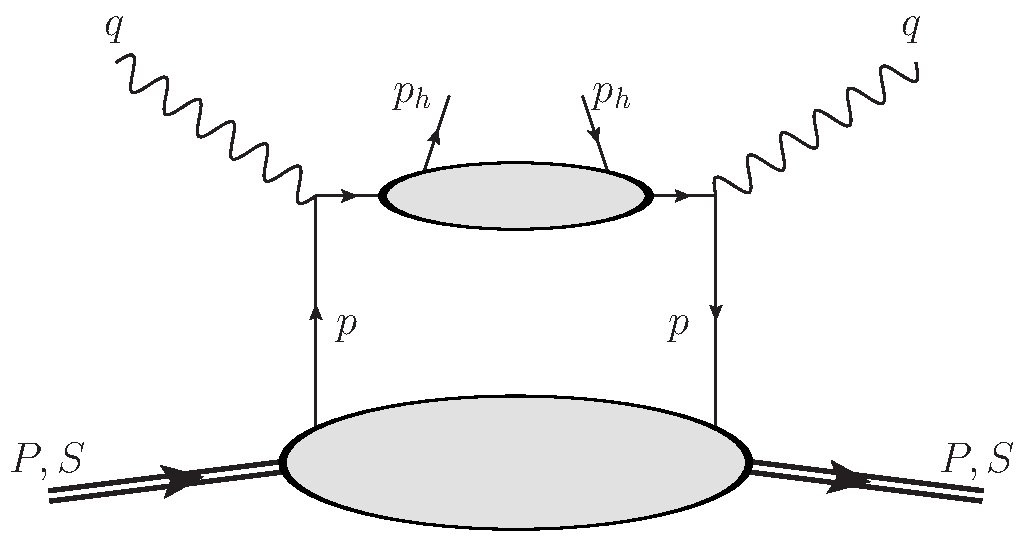
\includegraphics[width=0.5\textwidth]{SIDIS_2.pdf} 
  \caption{Parton model for SIDIS.}
  \label{fig:SIDIS_PM}
\end{figure}

The kinematic variables are the same of DIS, Eqs.~(\ref{eq:nu}-\ref{eq:W2}), with the additional variable
%%
\begin{equation}
  z = \frac{P \cdot p_h}{P \cdot q} \,,
\end{equation}
%%
where $p_h$ is the four-momentum of the detected hadron. The PM approximation of the process is displayed in Fig.~\ref{fig:SIDIS_PM}.\par
For collisions with longitudinally polarised leptons and targets, the polarised structure function can be isolated by taking the difference between the cross-sections with opposite target helicities \cite{Abele:2021nyo}
%%
\begin{equation}
  \frac{d \Delta \sigma^h}{dx \, dy \, dz} \equiv  \frac{1}{2} \left(\frac{d^3\sigma_{h}^{\uparrow \Uparrow}}{dx\,dy\,dz} - \frac{d^3\sigma_{h}^{\uparrow \Downarrow}}{dx\,dy\,dz}\right) = \frac{4\pi \alpha_{em}^2}{Q^2} (2-y) g_{1}^{h} (x,\,z,\,Q^2)\,.
\end{equation}
%%
As for DIS, it can be proved (see \textit{e.g.} Ref.~\cite{collins_2011}) that a factorisation theorem holds also for SIDIS processes. The structure function $g_1^h (x,z,Q^2)$ may be written as
%%
\begin{equation}
  \begin{split}
    g_1^{h} (x,z,Q) & = \frac{1}{2} \sum_{q,\bar{q}} e_{q}^2 \left[ \Delta q(x,Q) \otimes \Delta \mathcal{C}_{qq}^{1} \otimes D_{q}^{h}(z,Q) + \right.\\
    & \left.\Delta q(x,Q) \otimes \Delta \mathcal{C}_{gq}^{1} \otimes D^{h}_{g}(z,Q) + \Delta g(x,Q) \otimes \Delta \mathcal{C}_{qg}^{1} \otimes D^{h}_{q}(z,Q) \right] \,,
    \end{split}
    \label{eq:g1h}
\end{equation}
%%
where I have introduced the double convolution defined as 
%%
\begin{equation}
  f \otimes \Delta \mathcal{C} \otimes h (x,z) = \int \frac{d\xi}{\xi} \int \frac{d \zeta} {\zeta} f \left( \frac{x}{\xi}\right)  \, \Delta \mathcal{C} \left(\xi, \zeta\right) \, h \left( \frac{z}{\zeta} \right) \,.
\end{equation}
%%
In a certain sense, the FF "selects" the single flavour in the initial state. This has important phenomenological consequence in the parton determination, as I will discuss in Chap.~\ref*{ch:3}. Phenomenologically, the quantity that is measured in experiments is a normalised asymmetry, similar to Eq.~\eqref{eq:A1}, and takes the form~\cite{deFlorian:2000bm}
%%
\begin{equation}
  A_1^{h}(x,Q^2) \simeq  \frac{\int_{Z} dz \, g_1^h (x,z,Q^2)}{\int_{Z} dz \, F_1^h (x,z,Q^2)} \,,
\end{equation}
%%
where $Z$ denotes the kinematical region covered by final state hadrons.\par
Polarised coefficient functions have been computed at NLO in Ref.~\cite{deFlorian:1997zj} and up to (approximate) NNLO so far in Ref.~\cite{Abele:2021nyo}.%

Similarly to PDFs, FFs contain a $Q^2$-dependence which arises from the factorisation of the ultraviolet divergences. The perturbative dependence on the scale $Q^2$ is given by the same DGLAP equations, Eqs.~\eqref{eq:DGLAP_coupled}
%%
\begin{equation}
  \frac{\partial}{\partial \mu^2} D_{q_i}^{h} (z,\mu^2) = \frac{\alpha_s(\mu^2)}{2\pi} \sum_{j} \int_{z}^{1} \frac{du}{u} P_{ji}\left( u, \alpha_s(\mu^2) \right) \, D_{q_j}^h \left( \frac{z}{u}, \mu^2 \right) \,.
\end{equation}
%% 
The LO splitting function for FFs have been computed in Ref.~\cite{Owens:1978qz, Uematsu:1978yw, Georgi:1977mg}, and they are equivalent to the LO DGLAP splitting functions for PDFs. Splitting functions have been computed at NLO in~\cite{Curci:1980uw, Furmanski:1980cm}, and at NNLO in~\cite{Mitov:2006ic, Moch:2007tx, Almasy:2011eq}.
\chapter{Phenomenology of PDF determination}
\label{ch:3}

The aim of this chapter is to provide a brief review of the main methodological and numerical tools used in the determination of polarised parton distribution functions. The methodology used to carry out the present work is inspired by the framework developed by the NNPDF Collaboration. The code devoted to the determination of polarised PDFs, whose development has been the major work of this Thesis, goes by the name \texttt{Denali}, and it is provided by the MAP collaboration\footnote{\footnotesize MAP is an acronym that stands for \quotes{Multi-dimensional Analyses of Partonic distributions}. The GitHub page of the MAP Collaboration can be found at this link: \href{https://github.com/MapCollaboration}{https://github.com/MapCollaboration}.}. In Sec.~\ref{sec:gen_fit_str} I delineate the general strategy for PDF determination, focusing on the phenomenological issues. I will pay special attention to the technical problems that arise in the numerical implementation. Each issue will be then addressed in Sec.~\ref{sec:MAP}, in which I will present the methodological strategy.%

The contents presented in this chapter will set the stage for Chap.~\ref{ch:4}, in which the results will be discussed.

%___________________________________________________
\section{General approach to global QCD analysis}
\label{sec:gen_fit_str}

%%
\begin{figure}[t]
  \centering
  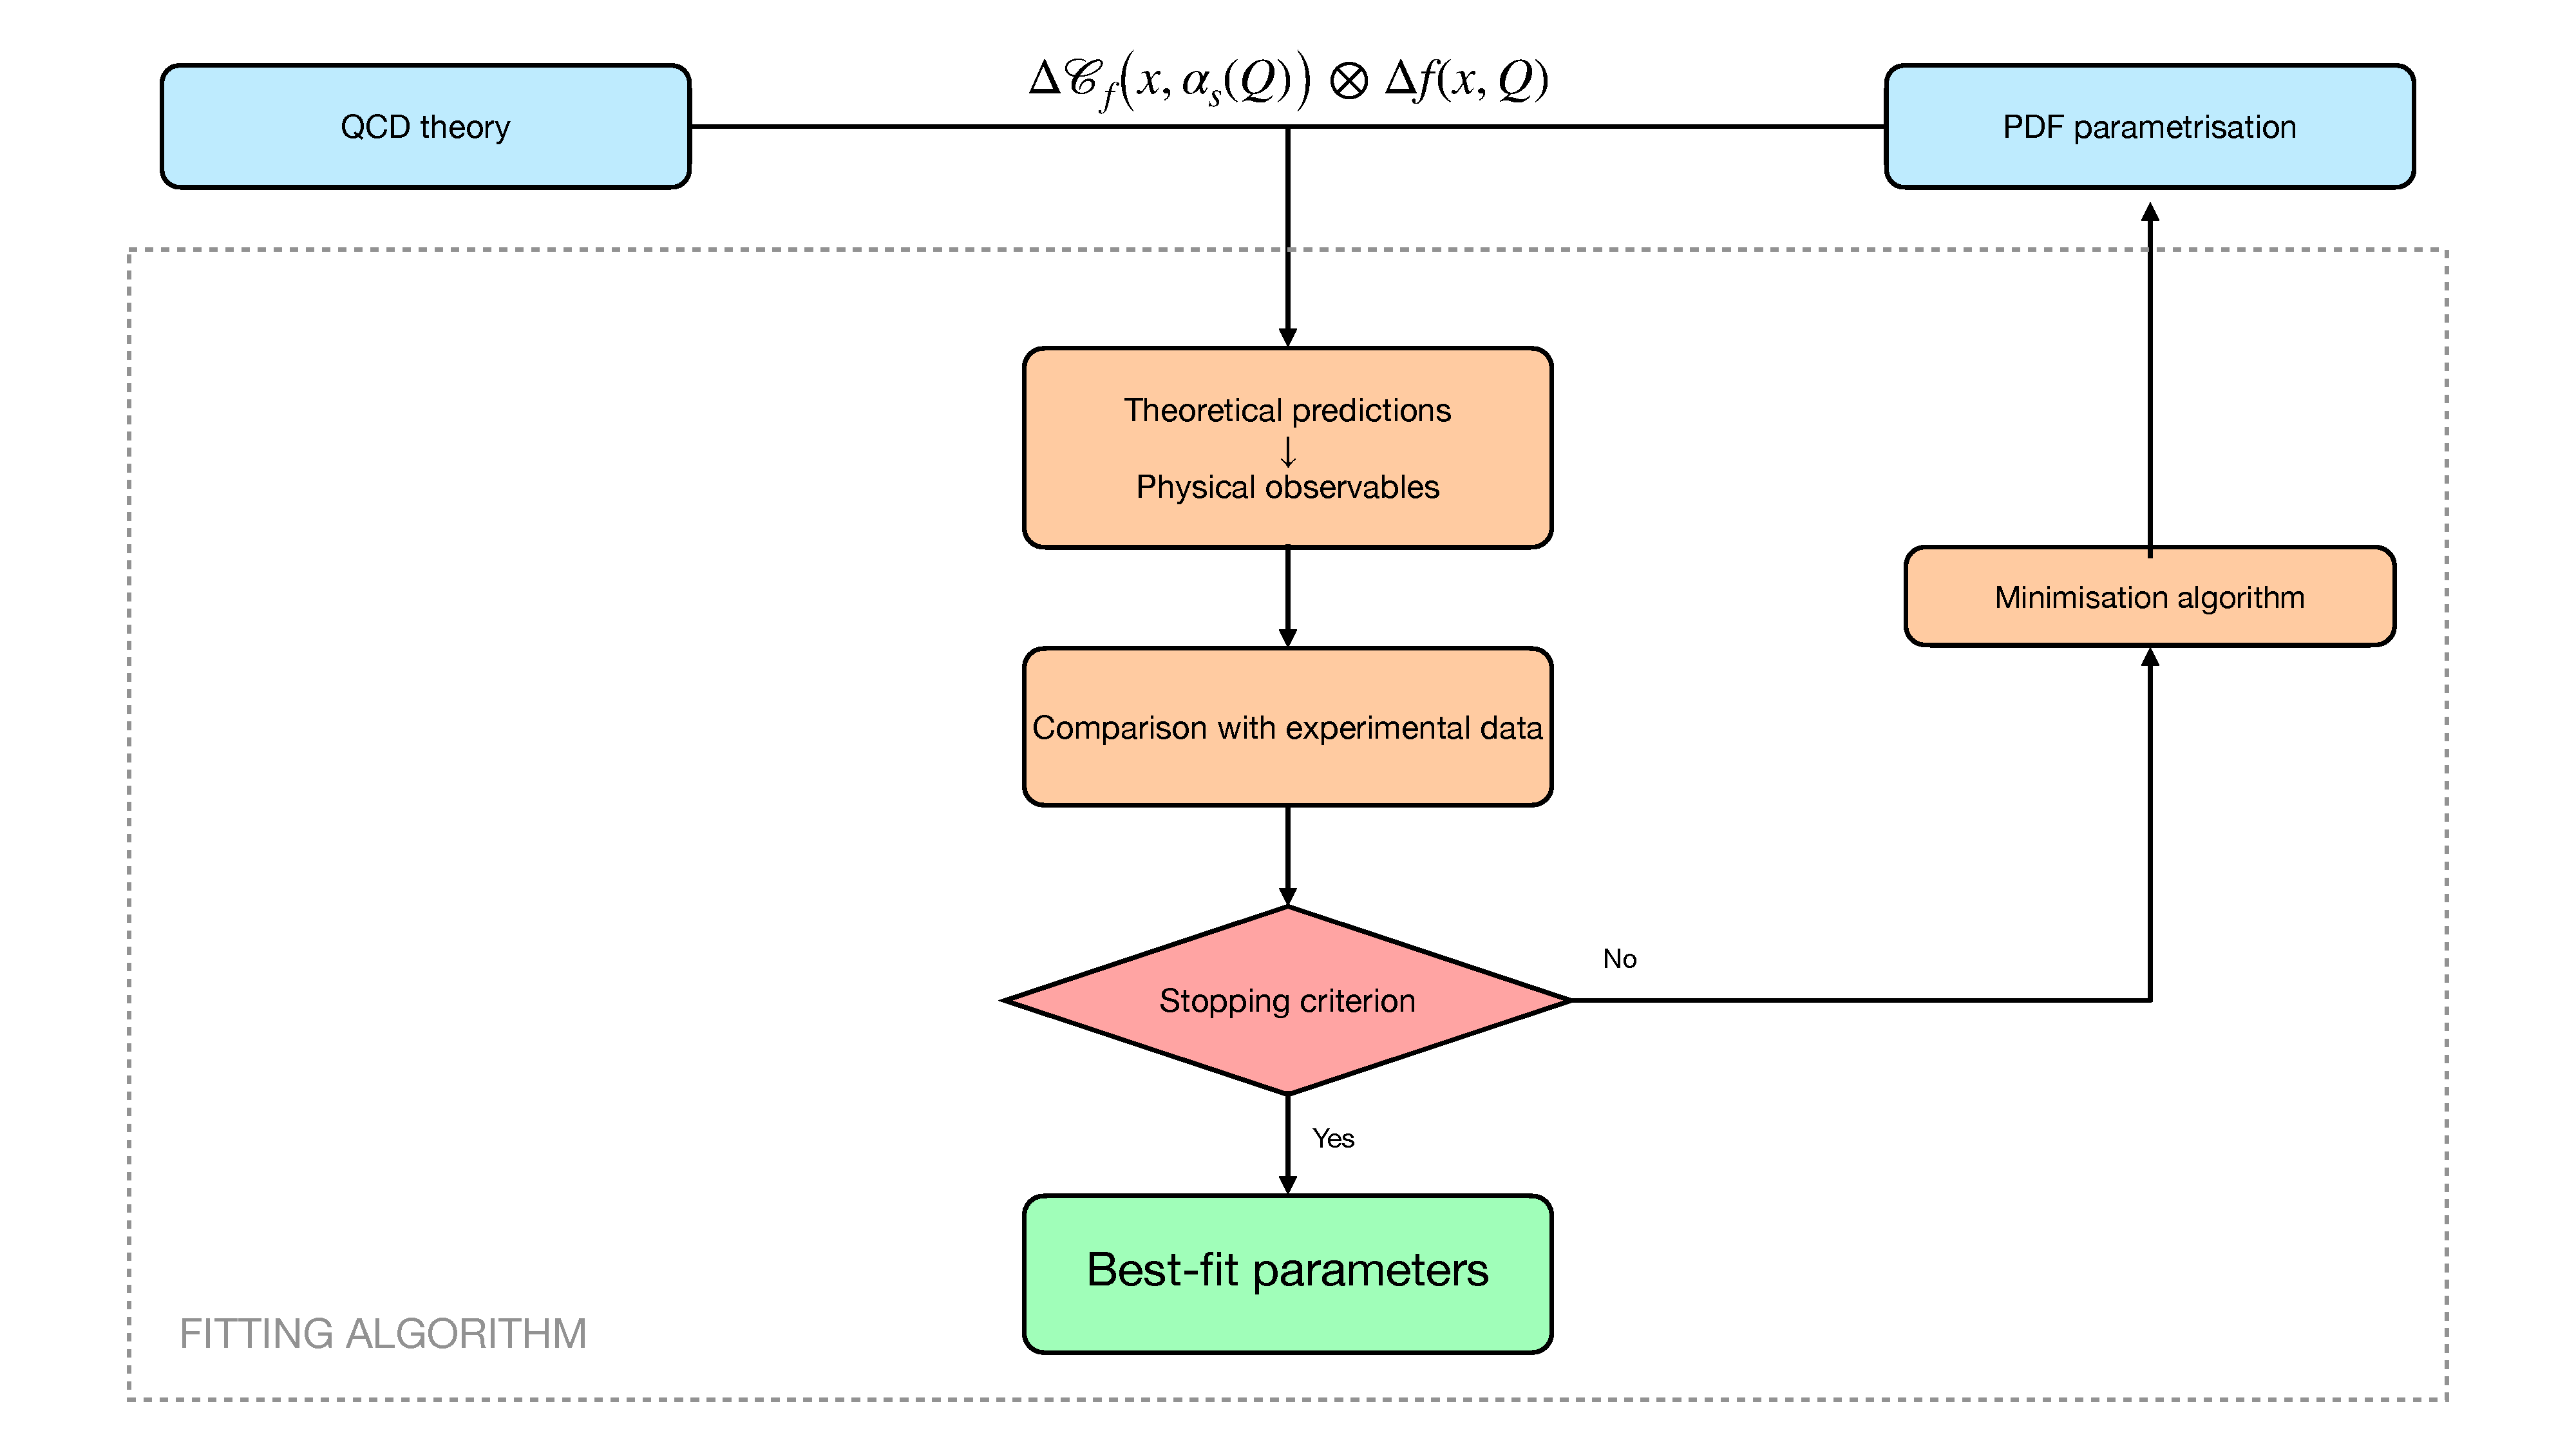
\includegraphics[width=1\textwidth]{fit_scheme.pdf} 
  \caption{Scheme of the general strategy for parton fitting.}
  \label{fig:fit_strategy}
\end{figure}
%%

The general strategy to determine PDFs in a global QCD analysis can be summarised as in Fig.~\ref{fig:fit_strategy}. Starting from the top, the factorisation theorem allows for the separation between the process-dependent partonic cross-section and the PDF. The former can be computed using the theoretical framework developed in Chap.~\ref{ch:2}, while the latter is parametrised by a certain function. Usually, PDF parametrisation is made at an initial energy scale $\mu_0$, and evolved to the energy scale of data by means of the DGLAP equations, Eqs.~\eqref{eq:DGLAP_coupled}.%

The set of measured observables $\left\{ \mathcal{O}^{\T{exp}}_i \right\}$ is compared with the corresponding set of theoretical predictions $\left\{ \mathcal{O}^{\T{th}}_i \right\}$. The agreement is quantified by a figure of merit (also known as \textit{error} or \textit{cost function}), usually chosen to be the $\chi^2$ (log-likelihood) function,
%%
\begin{equation}
  \chi^2 = \sum_{i,j}^{N_{dat}} \left( \mathcal{O}_{i}^{\T{(exp)}} - \mathcal{O}_{i}^{\T{(th)}} \right) \left[ \T{cov}_{ij} \right] \left( \mathcal{O}_{j}^{\T{(exp)}} - \mathcal{O}_{j}^{\T{(th)}}  \right) \,.
  \label{eq:chi2}
\end{equation}  
%%
where $\T{cov}_{ij}$ is the experimental covariance matrix. The reason for adopting the $\chi^2$ as error function relies on the assumption that data are independent and identically distributed, also known as \textit{i.i.d.} assumption. Then, Eq.~\eqref{eq:chi2} follows from the hypothesis that data are distributed according to a multivariate normal distribution, where the mean values are the experimental points and the covariance matrix is given by the experimental covariance matrix.%

Finally, the best fit is obtained by minimising the cost function by means of an optimization procedure. If the PDF parametrisation is such that the error function admits a close solution for the minimum, hence no stopping criterion is required. Otherwise, if no such close expression is possible, then the minimum is sought probing the parameter space by means of an iterative method. At each step, the stopping criterion applies a test to determine when to stop the iteration. In both cases, the best-fit parameters are those that minimise the error function and determine the shape of the PDF set.%

It should not surprise that the above picture, in spite of its apparent simplicity, hides several complications. Moreover, despite each issue seems to  affect a precise part of the machinery, they are strongly related to each other, contributing all together to the efficiency of the algorithm. I summarise these several issues in the following list.\\[10pt]
%%
\begingroup
\textbf{Numerical implementation and theoretical assumptions.} The first problem that parton fitting faces is the implementation of the theoretical framework developed in \chapref{ch:2}. Indeed, a single observable requires the computation of several convolutions, which can be a highly time-consuming task if not addressed with attention. Moreover, parton distributions must be evolved to the required energy scale, introducing an additional degree of complexity to the computation. Finally, it must be noted that the coefficient functions with which PDFs are convoluted include non-regular distributions, such as Dirac delta functions or plus-prescriptions. The solution to these problems is discussed in Sec.~\ref{subsec:APFEL}.
\\[6pt]
Other theoretical subtleties may arise from the QCD analysis discussed in Sec.~\ref{sec:field_theoretic}. For instance, heavy quark mass effects, as well as higher twist corrections, may modify the expression for the polarised structure function. However, both contributions can be mitigated and neglected by acting on the scale of the PDF parametrisation and implementing \textit{ad hoc} kinematic cuts to the data set, as it will be further discussed in \chapref{ch:4}.
\\[6pt]
Moreover, several theoretical constraints can be included in the analysis. For instance, the sum rules, Eqs.~(\ref{eq:a3_PM}-\ref{eq:a8_PM}), provide an additional constraint on the first moment of the non-singlet quark combinations. However, these relations require the assumption of exact $SU(2)_f$ and $SU(3)_f$ flavour symmetries, which in principle can be violated. Other constraints will be discussed later, and I will check whether these assumptions introduce a bias in the analysis.
\\[6pt]
Finally, it must be noted that the inclusion of processes involving identified hadrons in the final state introduces the dependence on the chosen set of FFs. For consistency, the perturbative order of the polarised PDF determination should match the perturbative order at which the FF determination has been carried out. A similar argument also holds for the unpolarised PDF set, which is included in the analysis in order to compute the polarised structure function and to impose the positivity constraint (for more details, see \chapref{ch:4}).
\endgroup
\\[10pt]
\begingroup
\textbf{Limited experimental data.} Each observable comes with its definition in terms of parton distributions (\textit{e.g.}, Eq.~\eqref{eq:g1_PM}). By using several observables related to different processes one can constrain different combinations of parton distributions. Thus, the experimental information used in a global fit should include different processes in order to constrain all the $(2 n_f + 1)$ independent parton components (where $n_f$ is the number of active flavours). If such an information is lacking, either the set of determined parton distributions is reduced or general assumptions on the unconstrained PDFs have to be made.
%Thus, the set of polarised PDFs that is possible to determine depends on the available experimental information. If such an information is lacking, either the set of determined parton distributions is reduced or general assumptions on the unconstrained PDFs have to be made.
\\[6pt]
The bulk of the experimental information concerning the polarised case comes from polarised inclusive DIS data. As discussed in Chap.~\eqref{ch:2}, the structure function related to this process only involves a particular combination of distributions, Eq.~\ref{eq:g1_NPM_ev}, mainly constraining the total quark distributions $\Delta u^{+}$, $\Delta d^{+}$ and $\Delta s^{+}$. The gluon distribution $\Delta g$ also enters the expression for the polarised structure function, although its contribution is suppressed by the running coupling, Eq.~\eqref{eq:g1_QFT}.
\\[6pt]
Recently, SIDIS data with polarised beams and targets have been released for various hadronic species (\textit{e.g.} $\pi^{\pm},K^{\pm}$). It is well known that the flavour of the originating parton, together with the charge of the hadron, strongly affect the FFs. As a consequence, it is possible to constrain alternative combinations of parton distributions by choosing the appropriate final hadron. It is then possible to achieve a full flavour decomposition for parton distributions. Still, the gluon contribution is not well constrained, given that it does not enter at leading order.
\\[6pt]
Finally, if compared to the unpolarised counterpart, polarised data are less precise and also less abundant, providing a rather limited kinematic coverage in the $(x,Q^2)$ plane. This has a strong impact on the precision of the determination.
\endgroup
\\[10pt]
\begingroup
\textbf{Functional parametrisation.} The choice of the parametrisation is the crux of the matter. It represents our ignorance of the non-perturbative nucleon structure and, for that reason, it must be carefully chosen. As a general rule, the parametrisation should be flexible enough to reproduce PDFs, avoiding (or limiting) any functional bias in the determination. 
\\[6pt]
Another issue related to the parametrisation is the \textit{generalisation} power, that is the ability of the model to predict new, previously unseen data. In that regard, the number of free parameters may have a considerable impact. A model with few parameters would be too limited and not able to acquire sufficient information from data. On the other hand, if such a number is excessively high, the parametrisation would be too flexible, and would start to model the noise of the data (\textit{i.e.} the model does not \quotes{generalise}). Thus, one must find the optimal balance between the high bias of a model that is too unflexible and the high variance of a model with too much freedom -- a problem also known as bias-variance trade-off.
\\[6pt]
Lastly, the functional form can be chosen to naturally implement some known behaviour, such as the behaviour at small-$x$ as suggested by Regge theory~\cite{Close:1994he} or the exact cancellation of the distributions at $x=1$.
\endgroup
\\[10pt]
\begingroup
\textbf{Error estimate.} Beside the functional parametrisation, another relevant issue is the PDF error determination. This can be achieved with the Hessian formalism \cite{Pumplin:2001ct}, or with the Lagrange multiplier method \cite{Stump:2001gu}. The former relies on the expansion about the minimum of the cost function, and requires the computation of the Hessian matrix, \textit{i.e.} the computation of the second derivative of the error function. The latter estimates the uncertainty by minimizing the error function with different values of a penality term. Both approaches involve massive computational tasks, either because of the difficulties encountered in computing the Hessian matrix, or because of the introduction of the penality term which strongly slows the speed of the fit. In addition, the Hessian method relies on the assumption that a first order, linear approximation is adequate, and error estimates based on this method are not necessarily always accurate.
\\[6pt]
A different approach is provided by the Monte Carlo sampling method, which is the one adopted for this analysis and will be discussed in Sec.~\ref{sec:MCS}. A comparison between these methods, with general details on each of them, can be found in Ref.~\cite{Forte:2010dt}.
\endgroup
\\[10pt]

\section{The fitting methodology}
\label{sec:MAP}
Having outlined the main issues involved in a global QCD analysis, I now present the methodology adopted to determine polarised PDFs. The determination is based on a Monte Carlo approach and the functional parametrisation is given by a feed-forward neural network (NN). The Monte Carlo sampling addresses the problem of the uncertainty estimation for all the observables related to polarised PDFs, while the NN provides an unbiased parametrisation of the distributions. The computation of the theoretical observables is handled by the \texttt{APFEL++} library, which tabulates the integrals that enter the analysis to create the so-called FK tables. Stochastic gradient descent (SGD) and cross-validation are used to train the network and to avoid the problem of \textit{overfitting}\footnote{\footnotesize It is worth mentioning that the problem of overfitting is only addressed by the cross-validation method. The SGD is an optimisation method whose primary purpose is to seek for the optimal solution in the minimisation problem. However, it has been shown by means of numerical experiments~\cite{2016arXiv160904836S} that SGD has side effects that seem to enhance the generalisation power of the model, in particular when a small batch of data is used to compute the gradient. So far, a clear explanation for this feature does not exist.}. A description of these tools is presented in the sections below.

\subsection{Numerical implementation: the \texttt{APFEL++} library}
\label{subsec:APFEL}
One of the issues that concerns a global analysis is the numerical implementation of the theoretical framework discussed in Chap.~\ref{ch:2}. Convolutions and evolutions are handled by the \texttt{APFEL++} library \cite{Bertone:2016lga,Bertone:2017gds}, whose methodology will be discussed here.%

In the context of collinear factorisation, the most relevant quantity that one has to compute is a Mellin convolution between an operator $\mathcal{O}$ and a distribution $d$, which I write here for convenience:
%%
\begin{equation}
  \mathcal{M}(x) = \int_{0}^{1} dy \int_{0}^{1} dz \; \mathcal{O}(y) d(z) \delta(x-yz) = \int_{x}^{1} \frac{dy}{y} \mathcal{O}(y) d \left( \frac{x}{y} \right)\,.
  \label{eq:def_conv2}
\end{equation}
%%
I will use $\mathcal{M}(x) \equiv \mathcal{O}(x) \otimes d(x)$ as shorthand notation for the convolution. The operator $\mathcal{O}$ contains the process-dependent perturbative contributions. Although its expression may become complicated at higher perturbative orders, it always shows the same mathematical structure: a \quotes{regular} term, whose integration into Eq.~\eqref{eq:def_conv2} does not present any difficulty, \quotes{local} terms proportional to $\delta(1-x)$, and \quotes{singular} terms, in which the singularity in $x=1$ is subtracted by means of the so-called plus-prescription. Such a complex structure makes the numerical computation of Eq.~\eqref{eq:def_conv2} rather expensive. On the other hand, the distribution $d$, which is the subject of interest in the present analysis, does not present any complication, given that it represents a $C^{\infty}$ smooth and continuous function (the PDF). The distribution $d$ can be easily accessed through the \texttt{LHAPDF} interface \cite{Buckley:2014ana}.%

In order to make the computation of the integral \eqref{eq:def_conv2} fast, the standard strategy is to use interpolation techniques and precompute the expensive part of the integral. First, the integration variable $z$ is discretised on a grid $g=\left\{ z_0,\dots, z_N\right\}$. Then, the distribution $d$ is interpolated over the grid $g$ by means of a set of interpolating functions:
%%
\begin{equation}
  d(z) = \sum_{\beta \in g} w_{\beta}(z) d_{\beta} \,,
  \label{eq:inter}
\end{equation}
%%
where $d_{\beta} \equiv d(z_{\beta})$ is the distribution $d$ evaluated on the interpolating point $z_{\beta}$ of the grid, whereas $w_{\beta}$ is the interpolating function associated to the $\beta$-th node. Usually, Lagrange polynomials are chosen as interpolating functions. After inserting Eq.~\eqref{eq:inter} into Eq.~\eqref{eq:def_conv2}, and assuming the value of $x$ to be equal to the $\alpha$-th node of the grid, the quantity $\mathcal{M}$ evaluated at $x_{\alpha}$ may be computed as a simple matrix product
%%
\begin{equation}
  \mathcal{M}_{\alpha} \equiv \mathcal{M}(x_{\alpha}) = \mathcal{O}_{\alpha \beta} d_{\beta} \,,
  \label{eq:vec_obs}
\end{equation}
%%
where the matrix $\mathcal{O}_{\alpha \beta}$ has been defined as
%%
\begin{equation}
  \mathcal{O}_{\alpha \beta} \equiv \int_{x_{\alpha}}^{1} \frac{dy}{y} \mathcal{O}(y) \, w_{\beta} \left( \frac{x_{\alpha}}{y}  \right) \,.
  \label{eq:matr_O}
\end{equation}
%%
In Eq.~\eqref{eq:vec_obs} a sum over repeated Greek indices is understood. Then, one can access an arbitrary value for $\mathcal{M}$ through the same interpolation technique:
%%
\begin{equation}
  \mathcal{M}(x) = \sum_{\alpha \in g} w_{\alpha}(x) \mathcal{M}_{\alpha} \,.
\end{equation}
%%
Hence, the integral Eq.~\eqref{eq:matr_O} can be tabulated once and for all, the computation of the observable $\mathcal{M}$ just amounts of a simple multiplication between a matrix and a vector. The operation thus becomes very fast and can be easily extended to any other distribution $d$.%

One can observe that the computation of an observable and the evolution share the same mathematical structure of Eq.~\eqref{eq:def_conv2}. Hence, both tasks can be recast into a unique set of tabulated values, providing the so-called Fast-Kernel (FK) tables.

\subsection*{Solution to DGLAP equations}
In Sec.~\ref{sec:field_theoretic} I have introduced the DGLAP equations, a set of $(2 n_f + 1)$ integro-differential equations that describe the evolution of PDFs (and FFs) with the scale $Q^2$. The kernel of this set of equations can be calculated in perturbative QCD, and at any order the mathematical structure is unchanged. Schematically, the equations can be written as 
%%
\begin{equation}
  \pdv{\Delta f_i(x, Q^2)}{\ln Q^2} = \int_x^1 \frac{dy}{y} P_{ij} \qty(\frac{x}{y}, Q^2) \; \Delta f_j(y,Q^2) \, ,
  \label{eq:DGLAPs}
\end{equation} 
%%
where the factor containing the coupling constant has been neglected and the factors in the RHS of Eq.~\eqref{eq:DGLAP_coupled} is contracted into a single term $P_{ij}$. In the following, the latin indexes run over quark and antiquark flavours together with the gluon ($i=u,d,\dots \bar{u},\bar{d}, \dots g$), whereas the greek indexes run over the nodes of the grid $g$.%

One can apply the same interpolation technique and interpolate the distribution $\Delta q_{i}(x,Q^2)$ as I did in Eq.~\eqref{eq:inter}. In doing so, Eq.~\eqref{eq:DGLAPs} acquires a simple form
%%
\begin{equation}
  \pdv{\Delta f_i(x_{\alpha},Q^2)}{Q^2} = \sum_{\beta} \Pi_{ij,\alpha \beta} (Q^2) \; \Delta f_j(x_{\beta}, Q^2) \,,
  \label{eq:DGLAP_recast}
\end{equation}
%%
where the matrix $\Pi_{ij,\alpha \beta}$ is defined as in Eq.~\eqref{eq:matr_O} and reads
%%
\begin{equation}
  \Pi_{ij,\alpha \beta} (Q^2) = \int_{x_{\alpha}}^1 \frac{dy}{y} P_{ij} \qty(\frac{x_{\alpha}}{y}, Q^2) \; w_{\beta}^{(k)} (y)\,.
\end{equation}
%%
The functions $w_{\beta}^{(k)}$ are Lagrange polynomials of degree $k$ used as interpolating function. If one assumes that $\Delta f_i(x_{\beta},Q^2) \equiv \Delta f_{i,\beta}(Q^2)$ evolves between the energies $Q^2$ and $Q^2_0$ according to
%%
\begin{equation}
  \Delta f_{i,\beta} (Q^2) = \sum_{k} \sum_{\gamma} \Gamma_{ik,\beta \gamma} (Q^2,Q^2_0) \, \Delta f_{k,\gamma} (Q^2_0) \,,
  \label{eq:disc_evol}
\end{equation}
%%
provided that the boundary condition $\Gamma_{ik,\beta \gamma} (Q^2_0,Q^2_0) = \delta_{ik} \delta_{\beta \gamma}$ is satisfied, then the evolution operator in Eq.~\eqref{eq:disc_evol} satisfies the following differential equation
%%
\begin{equation}
  \frac{\partial \Gamma_{ij,\alpha \beta} }{\partial \ln Q^2} (Q^2,Q^2_0) = \sum_{k} \sum_{\gamma} \Pi_{ik,\alpha \gamma}(Q^2) \, \Gamma_{kj,\gamma \beta}(Q^2,Q^2_0)  \,,
  \label{eq:sys_DGLAP_kernel}
\end{equation}
%%
which is a first order linear differential equation. It can be solved with standard numerical algorithms, such as the Runge-Kutta methods.\par

\subsection*{Fast-Kernel tables}
It is now possible to present the numerical implementation of the calculations of the structure functions. In the framework of DIS, the polarised structure function $g_1$ can be decomposed as 
%%
\begin{equation}
  \begin{split}
    g_1(x,Q^2) & = \sum_{i=q,\bar{q},g} \Delta \mathcal{C}_{i}(x,Q^2) \otimes \Delta f_i (x,Q^2) \\
    & = \sum_{i=q,\bar{q},g} \Delta \mathcal{C}_{i}(x,Q^2) \otimes \Gamma_{ij} (Q^2,Q^2_0) \otimes \Delta f_i (x,Q^2_0) \,,
  \end{split}
\end{equation}
%%
where $\Delta \mathcal{C}_{i}(x,Q^2)$ are the process-dependent coefficient functions that I discussed in Sec.\ref{sec:field_theoretic}. $\Gamma_{ij} (Q^2,Q^2_0)$ is the evolution operator that I introduced earlier and that evolves the distribution from the initial parametrisation scale $Q^2_0$ to the hard-scattering scale $Q^2$. Finally, $\Delta f_i$ is the polarised PDF of flavour $i$ evaluated at the initial scale $Q^2_0$ and $\otimes$ denotes the usual Mellin convolution, Eq.~\eqref{eq:def_conv2}. Since the direct calculation is numerically expensive, one can exploit the methodology previously discussed. Indeed, 
%%
\begin{equation}
  \begin{split}
    g_1 (x_{\alpha},Q^2) & = \sum_{i} \mathcal{O}_{i,\alpha \beta}(Q^2) \Delta f_{i,\beta}(Q^2) \\
    & = \sum_{i,k} \sum_{\beta, \gamma} \mathcal{O}_{i,\alpha \beta}(Q^2) \Gamma_{ik,\beta \gamma} (Q^2,Q^2_0) \Delta f_{k,\gamma}(Q^2_0) \\
    & = \sum_{k} \sum_{\gamma} \left( FK \right)_{k, \alpha \gamma} (Q^2,Q^2_0) \Delta f_{k, \gamma}(Q^2) \,,
    \label{eq:g1_FK}
  \end{split}
\end{equation}
%%
where the information about the partonic cross-sections and the DGLAP evolution are encoded into the FK tables, defined as
%%
\begin{equation}
  FK_{k, \alpha \gamma}  (Q^2, Q^2_0) \equiv \sum_i \sum_{\beta} \mathcal{O}_{i,\alpha \beta}(Q^2) \Gamma_{ik,\beta \gamma} (Q^2, Q^2_0)\,.
\end{equation}
%%
As a result, the series of convolutions are expressed in terms of simple matrix multiplications that can be easily handled numerically. Moreover, the tabulation of the FK tables can be done once and for all at the beginning of the fit, improving the speed and the memory efficiency of the algorithm.%

In case of double convolutions, as for the SIDIS observables, this procedure still holds. It turns out that the coefficient functions for SIDIS have a clear separation of the kinematic variables $x$ and $z$, concerning the PDFs and the FFs, respectively. Hence, the double convolution is simply transformed into a product of two convolutions, each of them bearing separately the dependence either on $x$ on in $z$. 


%___________________________________________
\subsection{Neural Network parametrisation}
\label{sec:NN}

Polarised PDFs are parametrised in terms of a neural network. In the context of PDF determination, neural networks have been used for the first time by the NNPDF collaboration \cite{Forte:2002fg}. For the current analysis, I will deal with feed-forward neural network, although other architectures can be used (see \textit{e.g.} \cite{Bishop}). The part of the code concerning the parametrisation with neural networks, and that also provides an efficient way to compute the analytic derivatives, is handled by \texttt{NNAD}~\cite{AbdulKhalek:2020uza}.%

Neural networks are a neural inspired nonlinear model for supervised learning. Basically speaking, neural network models can be regarded as a series of nonlinear transformations. The building blocks of a network are the \textit{neurons} (or $\textit{nodes}$), organised in \textit{layers}, with the output of one layer serving as the input for the next one. The first layer of the network is the \textit{input} layer, whereas the final one corresponds to the \textit{output} layer. All the layers in the midst are called \textit{hidden units} (or \textit{hidden layers}).\par
Starting from the input layer, one can construct $N_1$ linear combinations of the input variables $x_1, \dots, x_N$ and obtain:
%%
\begin{equation}
  a_j = \sum_{i=1}^{N} w_{ij}^{(1)} x_i + \vartheta^{(1)}\,,
  \label{eq:activation}
\end{equation}
%%
where $j=1,\dots,N_1$ and the subscript $(1)$ indicates that the corresponding parameters are related to the first layer (the one immediately after the input layer) of the NN. The parameters $w^{(1)}_{ji}$ are usually known as \textit{weights} and the parameters $\vartheta^{(1)}$ as \textit{biases}. Together with the input variables, they contribute to the construction of the quantity $a_j$, also known as \textit{pre-activation}. The latter serves as argument of a differentiable, nonlinear \textit{activation function} $h$ to give
%%
\begin{equation}
  z_{j} = h(a_j)\,,
\end{equation}
%%
hence providing a functional (nonlinear) transformation of the pre-activation. The outputs of these transformations serve as input for the nodes that compose the next layer.%

The procedure that I have just discussed can be iterated, provided that a new set of weights and biases in introduced. Given a NN with $L$ layers and $N_{\ell}$ nodes in the $\ell$-th layer, the output of the $i$-th neuron in the $\ell$-th hidden layer can be written as
%%
\begin{equation}
  z_{i}^{(l)} = h \left( \sum_{j=1}^{N_{l-1}} w_{ij}^{(l)} z_{j}^{(l-1)} + w_{i0}^{(l)} \right) \,,
  \label{eq:activity}
\end{equation}
%%
In the terminology adopted, the input layer is denoted by $l=1$, the output layer with $l=L$, and the hidden layers with $l=2,\dots,L-1$.%

In order to properly approximate a continuous function, the activation function in the neural network must be nonlinear. Indeed, if all the hidden units in the network were taken to be linear, then it would be possible to find a single linear transformation equivalent to the network. This is a direct consequence of the fact that the composition of successive linear transformations is itself a linear transformation.%

The simplest example of activation function is the step function $\Theta(x)$, which acts as a binary activator. With this choice, the neural network can be seen as made of multiple layers of \textit{perceptrons}, which are discriminative functions in linear models for classification. For this reason, the name \textit{multilayer perceptron} is used to indicate this type of configuration. However, one is led to use continuous nonlinear functions instead of nonlinear step-function. In doing so, the neural network becomes differentiable with respect to the parameters. This property is fundamental in network training, and it is exploited by \texttt{NNAD} to compute the gradient of the network over the parameter space. The most popular activation function is the sigmoid
%%
\begin{equation}
  h(a) = \frac{1}{1 - e^{-a}}\,,
  \label{eq:sigmoid}
\end{equation}
%%
which presents two distinct regimes — linear and nonlinear. The linear response is obtained when the argument is approximatively near the origin, $a \approx 0$, whereas it saturates for large positive and negative values. If the parameters are such that the sigmoid works on the crossover between linear and saturation regimes, the nonlinearity of the NN is restored.\par
Globally, a neural network can be seen as a function of the set of weights $\{ w^{(l)}_{ij} \}$ and biases $\{ \theta_{i}^{(l)} \}$, together with the inputs $\left\{  x_i\right\}$
%%
\begin{equation}
  \vb*{z}^{(L)} \equiv f \left( \vb*{w}, \vb*{x}; \, h \right) \,.
  \label{eq:NN_func}
\end{equation}
%%
The process of evaluating Eq.~\eqref{eq:NN_func} is a forward propagation, since the information of the input layer is propagated through the network with continuous transformations. For that reason, such an architecture is known as \textit{feed-forward neural network}. It must be observed that I consider only neural networks in which the previous layer is connected only with the consecutive layer. Other feed-forward topologies, however, are possible.%

The choice of the activation function in the output layer is determined by the nature of the problem that one has to address. Among many possible options, the most popular are linear functions, the sigmoid, or the identity. However, in the next chapter I will show that this arbitrariness allows one to choose the output function in order to implement physical constraints analytically, improving the efficiency of the algorithm.%

Given the high number of parameters that enter the neural network, the functional form is redundant enough not to introduce a methodological bias which would artificially reduce parton uncertainty in regions where data do not constrain PDFs enough.


%______________________________________________
\subsection{Network training and optimisation}
\label{sec:NNtr}
After defining the general structure of the network parametrisation, I now address the delicate issue of finding the set of parameters that minimises the error function. In the context of neural network, the optimisation of the parameter space is also known as \textit{network training}. The first step of the network training is the minimisation of the error function. Since it is a smooth continuous function of the parameters, its smallest value occurs at a point in parameter space such that the gradient of the error function vanishes. However, given the high nonlinearity of the error function w.r.t. the parameters, there could be different local minima. Since it is clearly impossible to find an analytical solution to the equation $\nabla \chi^2 = 0$, one must resort to iterative numerical procedures that probe the space of parameters. The basic idea is that a small step in weight space reflects in a change of the error function. Thus, in order to find the minimum of the error function, one can start from a random initialised set of parameters and then move through the weight space in a succession of steps. The standard choice is to use the so-called gradient descent (GD) method, in which the minimum is sought by moving along the direction of the negative gradient of the cost-function
%%
\begin{equation}
  \vb*{w}^{\tau + 1} = \vb*{w}^{\tau} - \eta \nabla \chi^2 (\vb*{w}^{(\tau)}) \,,
  \label{eq:GD}
\end{equation}
%%
where $\tau$ labels the iteration step and $\eta$ is the \textit{learning rate}. However, for this analysis the stochastic gradient descent (SGD) is adopted. Stochasticity is incorporated by computing the gradient on a subset of the data called \textit{minibatch}. The impact of this variation of GD method is twofold: first, it introduces stochasticity and decreases the chance that the fitting algorithm gets stuck in isolated local minima. Second, it significantly speeds up the calculation as one does not have to use all the data points to approximate the gradient.%

The reason that leads one to use gradient information in the minimisation procedure is that the gradient of the error function can be computed efficiently by means of the \textit{backpropagation} procedure. It relies on the ordinary chain rule for partial differentiation. Indeed, the cost function depends directly on the activities of the output layer $z_j^{(L)}$, but also indirectly on all the activities of neurons in lower layers through iteration of Eq.~\eqref{eq:activity}. Hence, the gradient of the cost function w.r.t. the weights and biases of each layer can be obtained by applying consecutively the chain rule through the network, starting from the output layer. In other words, one is \quotes{backpropagating} the error starting with the top layer down to the input layer and uses these intermediate errors to calculate the desired gradients \cite{HBLV}. Of course, this technique requires the knowledge of the derivative of the cost function with respect to the activities of the output layer, which is not always the case. However, it can be shown that using the $\chi^2$ as error function, a close and analytical expression for the gradient does exist \cite{AbdulKhalek:2020uza}. Such a computational efficiency is fundamental since the gradient must be computed at each step of the gradient descent.%

Finally, one can observe that the purpose of a neural network is not only approximation, but also prediction. That is to say, one wants the predictions of the network to be comparable with a set of data the has not been used for training. This is correlated to another subtle problem, known as \textit{overlearning}, due to the high redundancy and flexibility of the network. In presence of overlearning, it starts to fit statistical noise of the data, rather than the underlying physical law. This affects the prediction power, since the statistical noise is characteristic of each data set. The solution to this additional complication is achieved using a cross-validation method, which introduces a criterion that stops the fit before it starts to overlearn. The technical details for this implementation will be discussed in \secref{sec:4.3}.


%___________________________________________
\subsection{Monte Carlo sampling}
\label{sec:MCS}
%%
\begin{figure}[t]
  \centering
  \begin{subfigure}[b]{0.45\textwidth}
      \centering
      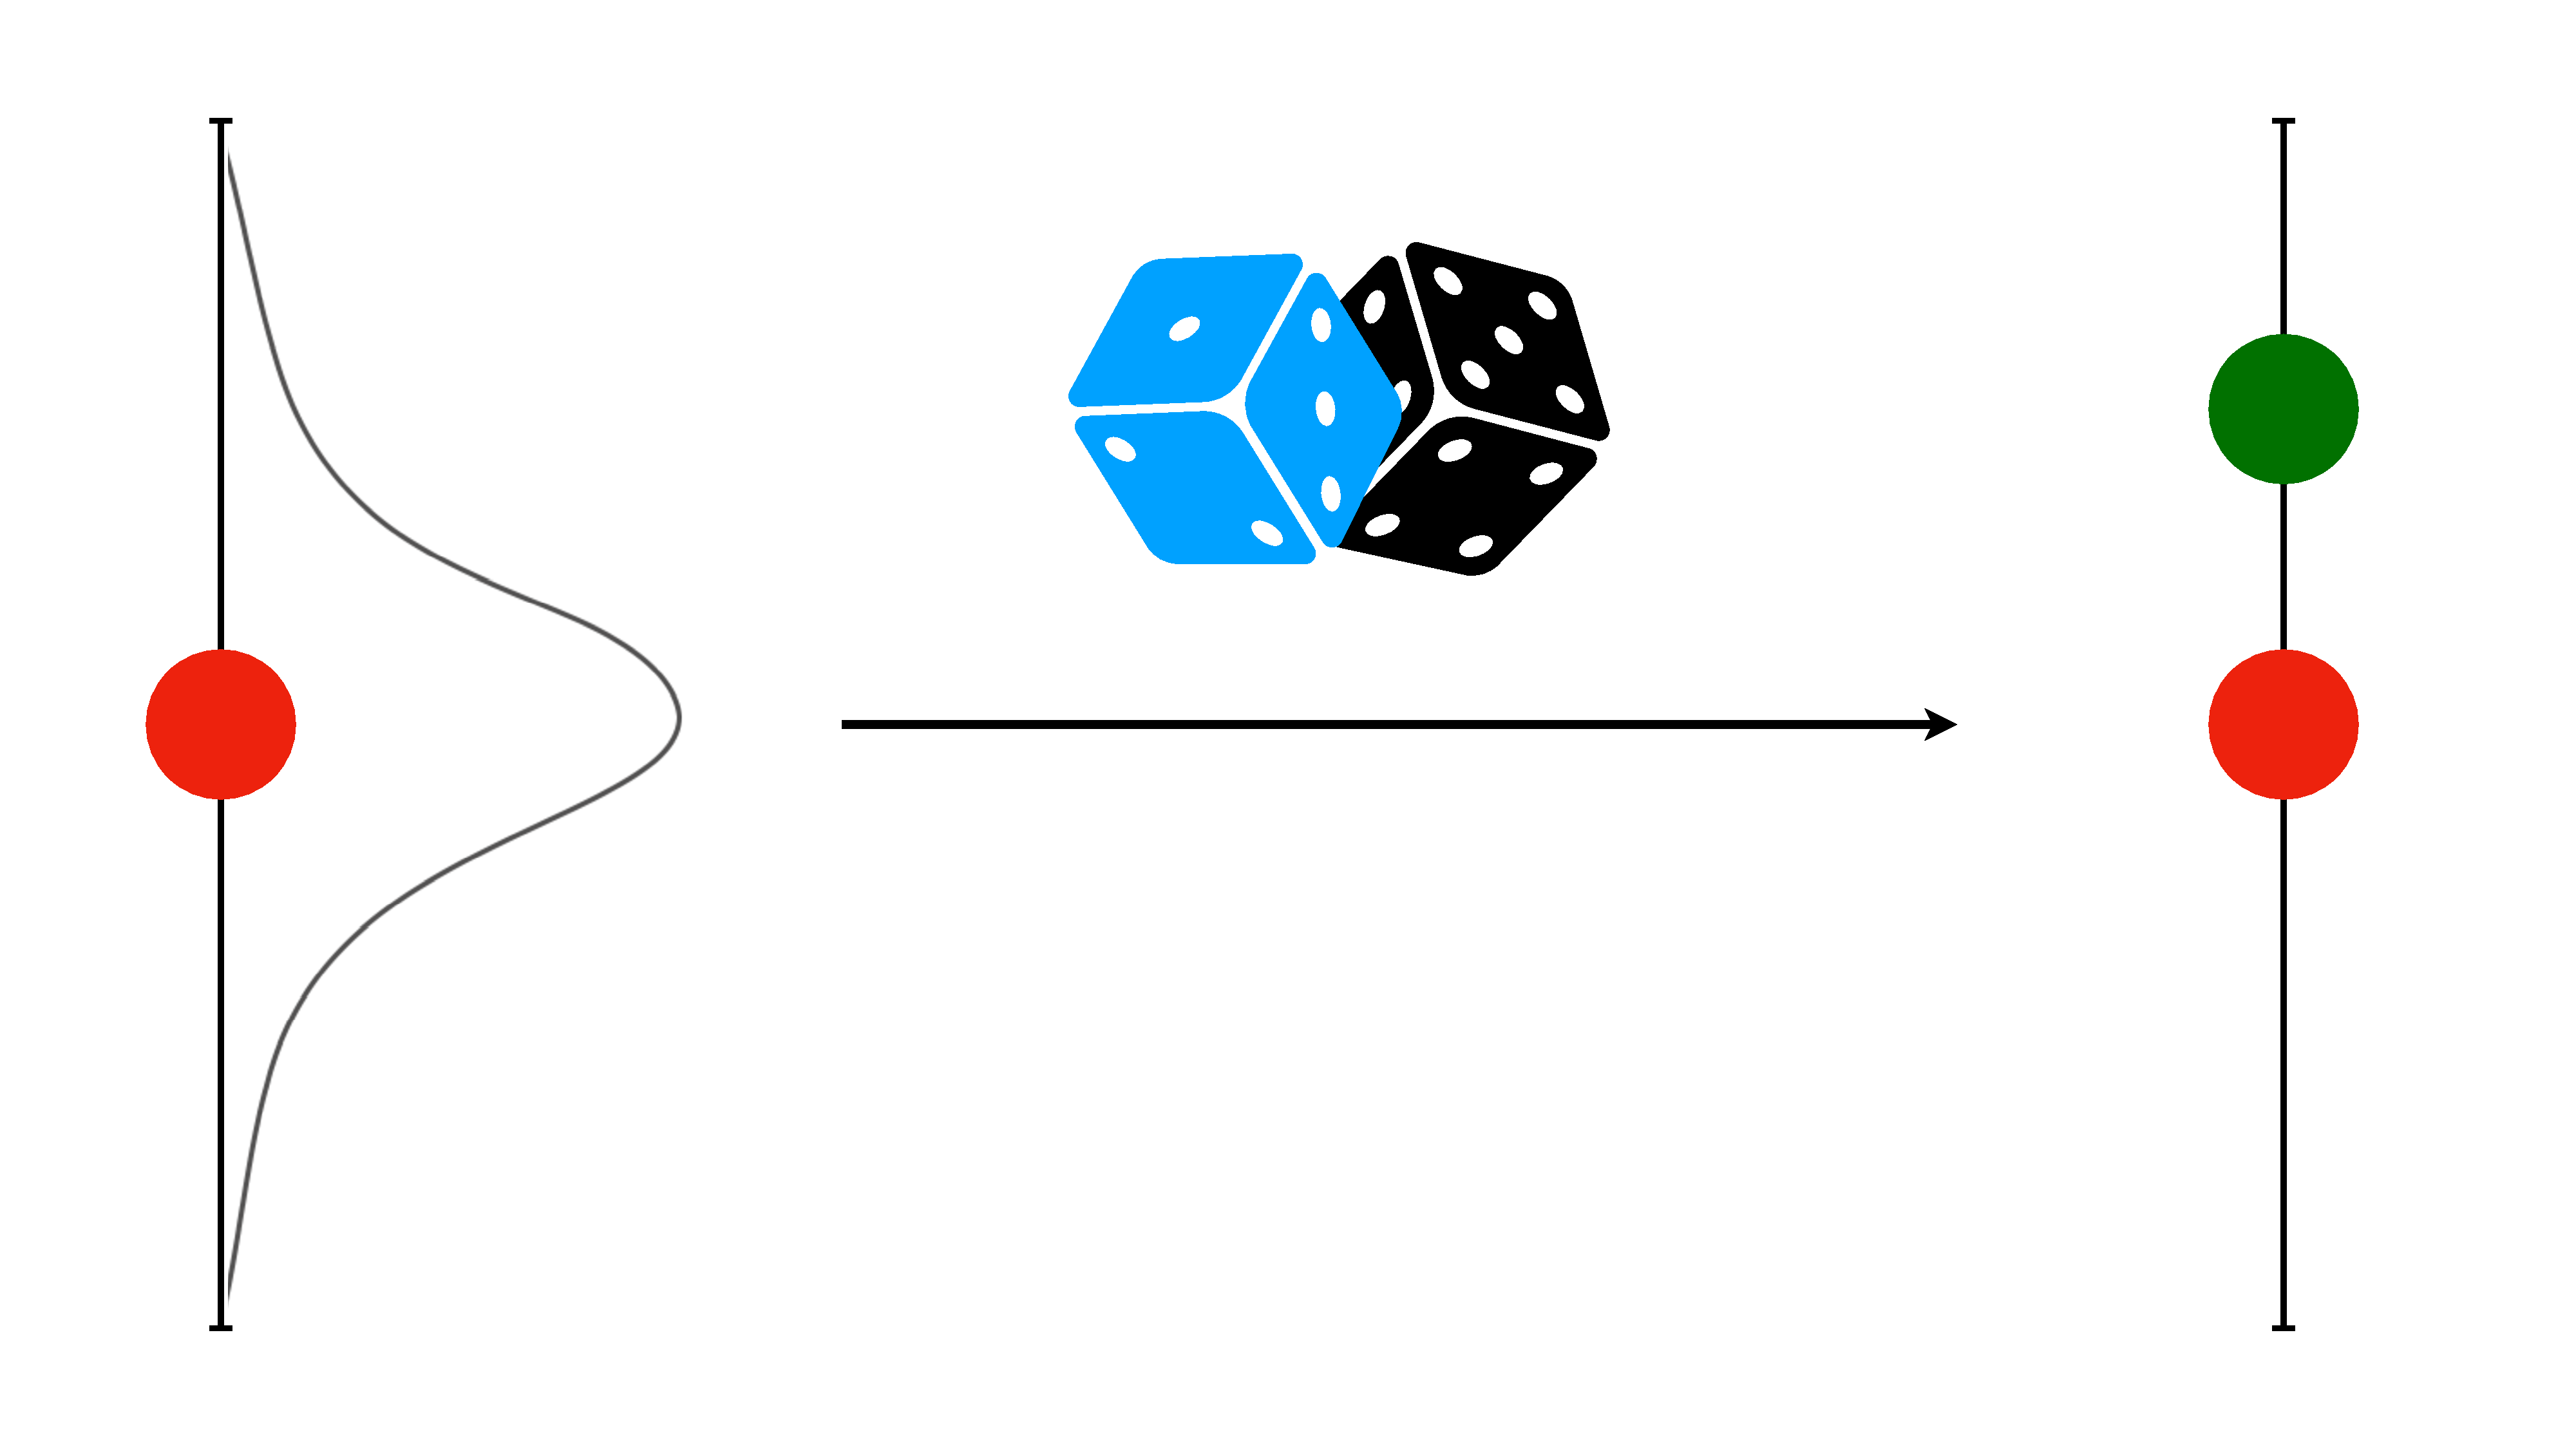
\includegraphics[width=\textwidth]{MC_fluc.pdf}
      \caption{The fluctuation process. The red dot is the central value; the green dot is the artifical value.}
      \label{fig:MC_fluc}
  \end{subfigure}
  \hfill
  \begin{subfigure}[b]{0.45\textwidth}
      \centering
      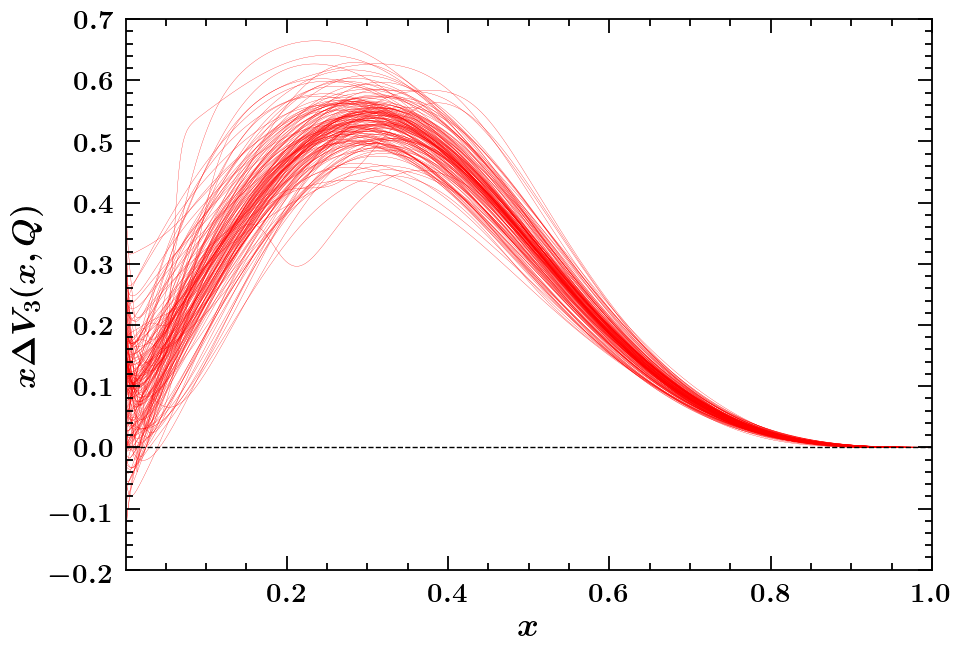
\includegraphics[width=\textwidth]{replica.png}
      \caption{Ensemble of polarised PDFs.}
      \label{fig:PDF_ensemble}
  \end{subfigure}
     \caption{Representation of the Monte Carlo Sampling}
     \label{fig:MC_2_Gr}
\end{figure}
%%
The average of an observable that depends on polarised PDFs $\mathcal{O}(\Delta f_i)$ is given by integrating the observable itself in the functional space $\mathcal{V}\left( \left\{ \Delta f_i \right\}\right)$ spanned by the parton distributions, weighted by the probability measure $\mathcal{P}\left(\{\Delta f\}\right)$ to observe a PDF at some reference scale, that is \cite*{Nocera:2014vla}
%%
\begin{equation}
  \left< \mathcal{O}(\Delta f) \right> = \int_{V} \mathcal{D} \Delta f \; \mathcal{P}\left( \{\Delta f \}\right) \; O \left[ \Delta f \right] \,.
\end{equation}
%%
Although the analytical expression for the probability measure $\mathcal{P}\left( \{\Delta f \}\right)$ is not known\footnote{\footnotesize It is worth mentioning that for linear functions, a Bayesian approach to the solution of inverse problems can be used to obtain analytical expression for the probability measure $\mathcal{P}$~\cite{DelDebbio:2021whr}. However, the case of nonlinear problems is much more complicate and an analytical expression of the probability measure for a general nonlinear function does not exist thus far.}, one can sample this distribution by a Monte Carlo method.%

First, I generate an ensemble of replicas of the original data set, following the statistical distribution of the experimental data. Each artificial ensemble contains as many data points as are originally available in the data set. The process of creating the artificial data points from the distribution of the experimental data is called \textit{bootstrap}. I will refer to the original set as the unfluctuated data set. The statistical distribution of the experimental data contain all the experimental information, that is statistical and systematic uncertainties. In practice, most data are given with multivariate normal distributions, in which the uncertainties are contained in the covariance matrix and the mean value corresponds to the experimental central value. A sketch of the fluctuation procedure is shown in Fig.~\ref{fig:MC_fluc}. The number of replicas is chosen to faithfully reproduce the statistics of the original set, by means of statistical estimators that will be discussed in \secref{sec:4.1}.%

Then, for each artificial ensemble, parton distributions are fitted to the fluctuated data. Thus, at the end of the fit, one obtains a collection of PDFs with as many members as the number of replicas $N_{rep}$ generated from the data, Fig.~\ref{fig:PDF_ensemble}. Of course, each PDF replica will fluctuate according to the fluctuated data set used for the fit. However, this collection of PDFs replica serves as a statistical ensemble, from which one can compute the central value and the credibility interval. The smoothness of these two estimators increases with the number of artificial sets generated for the global fit.%
 
The advantages of the Monte Carlo methodology go further. Indeed, the expectation value of any observable that depends on polarised PDFs can be easily computed by averaging over the PDF ensemble to obtain
%%
\begin{equation}
  \left< O\left[ \Delta f \right] \right> = \frac{1}{N_{\T{rep}}} \sum_{k=1}^{N_{\T{rep}}} O\left[\Delta f^{(k)}\right] \,,
\end{equation}
%%
where $O\left[\Delta f_k\right]$ is the value of the observable computed out of the k-th PDF replica. In the same fashion, one can compute uncertainties such as the standard deviation
%%
\begin{equation}
  \sigma_{\mathcal{O}}^2 = \frac{1}{1 - N_{\T{rep}}} \sum_{k=1}^{N_{\T{rep}}} \left( \mathcal{O}[\Delta f^{(k)}] - \left< O\left[ \Delta f \right] \right> \right)^2 \,.
\end{equation}

\chapter{Polarised PDFs from DIS and SIDIS}
\label{ch:4}

In this Chapter, we present the first determination of polarised PDFs at next-to-next-to-leading order accuracy based on the MAP methodology, \texttt{MAPpol1.0}. The determination has been carried out including all available data from inclusive and semi-inclusive, neutral current, polarised DIS coming from different facilities. The final result will be a determination of light-flavours quark, antiquark, and gluon distributions at NNLO accuracy. In \secref{sec:4.1} we review the available data sets, and we discuss how pseudodata are generated in the context of the Monte Carlo method. The details of the analysis are discussed in \secref{sec:4.2}. In \secref{sec:4.3} we review the fitting strategy and discuss how the methodologies discussed in \chapref{ch:3} apply in our case. Finally, the \texttt{MAPpol1.0} parton set is presented in \secref{sec:4.4}, together with its stability upon the variation of some theoretical constraints.

\section{Experimental input}
\label{sec:4.1}

We review the experimental data sets used in the determination of the \texttt{MAPpol1.0} parton set, and we present how the uncertainties are taken into account. Then, we show the construction of the artificial ensemble of data points based on the Monte Carlo sampling method.

\subsection*{Data sets}
%%
\begin{figure}[t]
  \centering
  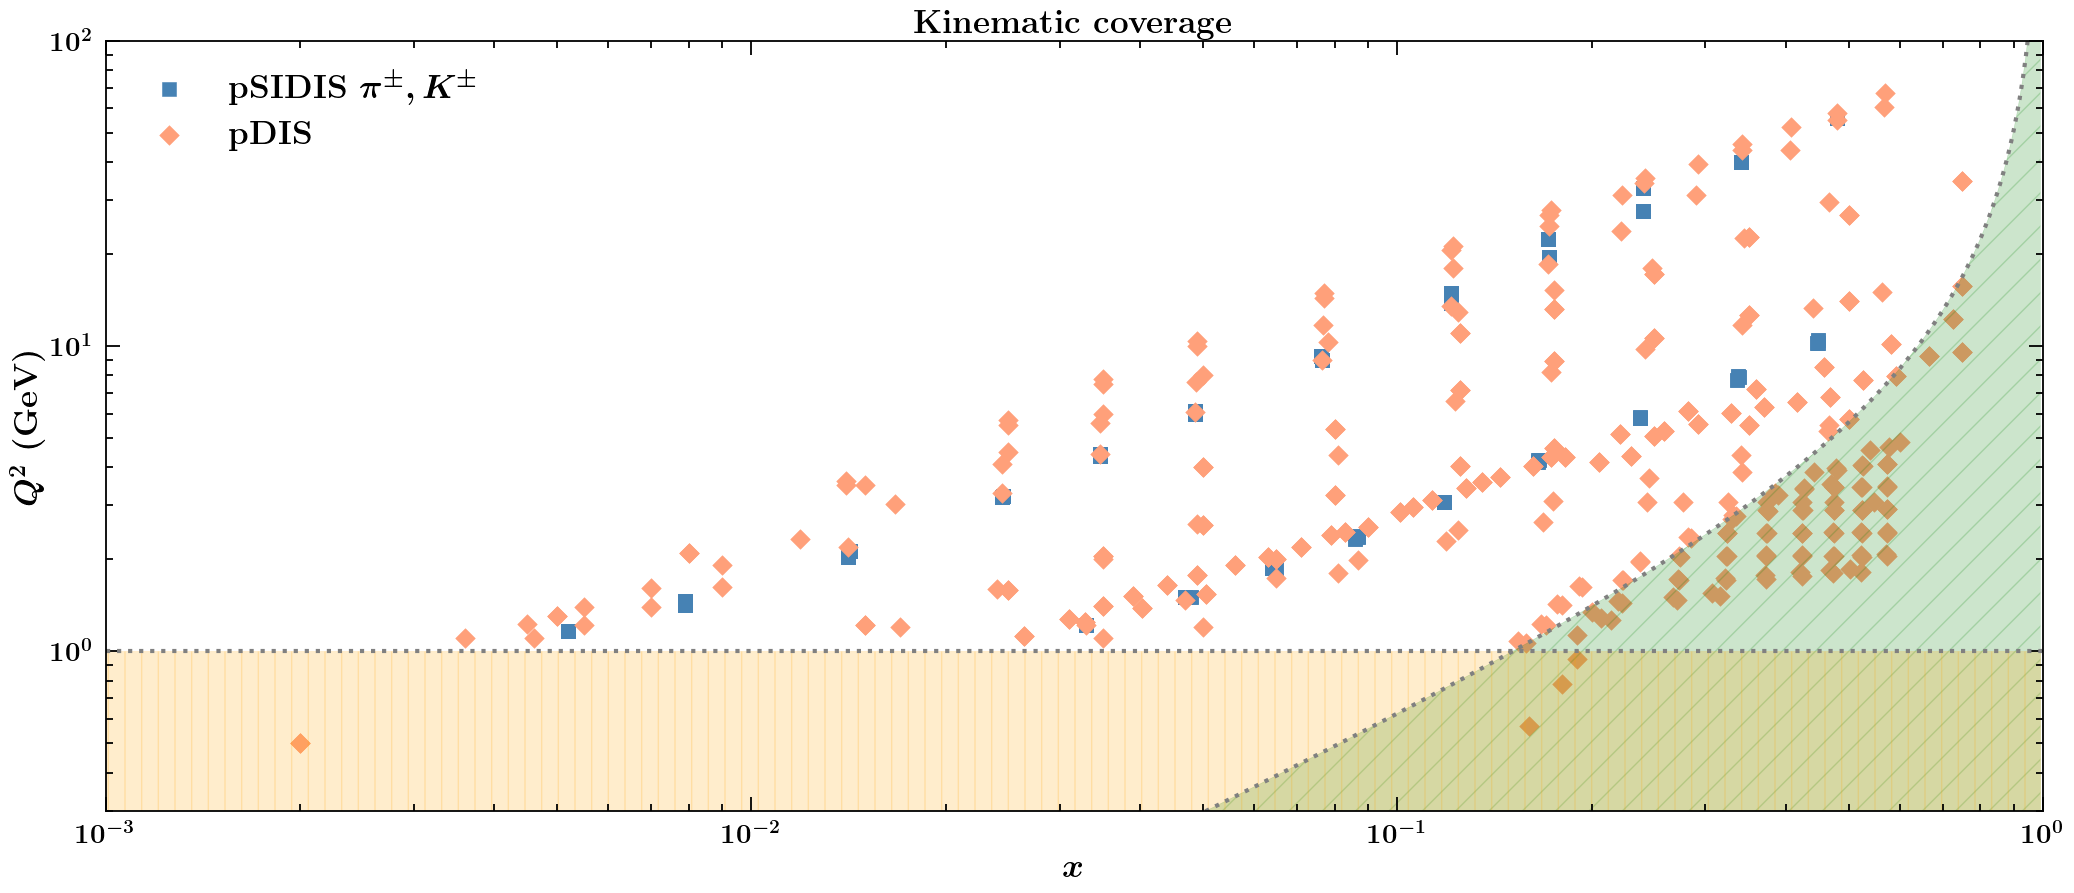
\includegraphics[width=1\textwidth]{kin_cov.png} 
  \caption{\small{Kinematic coverage in the $(x,Q^2)$ plane. The orange- and green-coloured areas represent the cuts in $Q^2$ and $W^2$, respectively.}}
  \label{fig:kin_cov}
\end{figure}
%%
In our analysis, we use inclusive and semi-inclusive lepton-nucleon DIS data coming from different facilities such as CERN \cite{EuropeanMuon:1989yki, Heiliger:1993qt, COMPASS:2006mhr, COMPASS:2010wkz, COMPASS:2010hwr}, SLAC \cite{E142:1993hql, E143:1998hbs, E154:1997xfa, E155:2000qdr}, DESY \cite{HERMES:2018awh, HERMES:2006jyl, HERMES:1997hjr} and Jefferson Lab \cite{Kramer:2002tt, JeffersonLabHallA:2004tea, CLAS:2014qtg}. For both DIS and SIDIS, the lepton beams are made of either electrons or muons. The targets are either protons or neutrons, and, in some case, deuterons. The main features of the data sets are summarised in Tab.~, in which we show the number of data points, the kinematic coverage, and the measured observables. The global kinematic coverage in the $(x,Q^2)$ plane is also shown in Fig.~\ref{fig:kin_cov}. \par
The observable that we use in the analysis is the (semi-)inclusive structure function $g_1^{(h)}$. However, some experiments provide its value normalised the unpolarised structure function, that is $g_1^{(h)}/F_1^{(h)}$. Thus, in computing the predictions, we must calculate the unpolarised structure function $F_1^{(h)}$, which introduces an additional dependence on the unpolarised parton set. The unpolarised set of PDFs adopted in the analysis is \texttt{NNPDF\red{which one?}}. We observe that some experiments publish many data tables with different observables, which eventually may be used to reconstruct the structure function of interest (see \textit{e.g.}, Ref.~\cite{Nocera:2014vla}).\par
In order to ensure the reliability of perturbative QCD, we exclude all data points with $Q^2 \leq Q^2_{\T{cut}} = 1 \, \T{GeV}^2$. This cut corresponds to the orange-coloured area of Fig.~\ref{fig:kin_cov}. In addition, we also impose a cut on the squared invariant mass of the hadronic final state $W^2$, in order to remove all the points that may be affected by higher-twist corrections, as discussed in \secref{sec:field_theoretic}. In particular, we will exclude points such that $W^2 \approx Q^2 (1-x)/x \leq W^2_{\T{cut}} = 6.5 \, \T{GeV}^2$. The excluded area  is shown in green in Fig.~\ref{fig:kin_cov}.\par
The resulting kinematic coverage is highly affected by these cuts. Starting from $480$ initially available points, after cuts this number reduces to $N_{\T{dat}}=360$,  -- a reduction of the $\sim 25\%$ respect to the initial points. We observe that the most affected experiments are those performed by Jefferson Lab \cite{Kramer:2002tt, JeffersonLabHallA:2004tea, CLAS:2014qtg}. Indeed, the cut in $W^2$ mainly affects all data points that cover the large-$x$ and small-$Q^2$ corner, which is exactly the region probed by these experiments.\par
Although the coverage of both low- and large-$x$ regions have been improved in recent years, the present situation for polarised data is not comparable with the unpolarised counterpart. This latter provides over than $3000$ data points coming from different processes other than DIS (see \textit{e.g}, Ref.~\cite{Kassabov:2022pps}). Moreover, the accuracy of these points is also better if compared to the unpolarised case. Still, this does not prevent us to perform a global determination, provided a reliable estimation of PDF uncertainties.\par
For each observable listed in Tab.~, the experiments provide information about their uncertainties.
In particular, correlated systematics (multiplicative and/or additive) are only given by E143, E155, EMC, and HERMES, whereas the other experiments only give uncorrelated uncertainties. With this information at our disposal, we can construct the covariance matrix $V_{ij}$ as follows
%%
\begin{equation}
  V_{ij} =  \sigma_{i,\T{unc}} \sigma_{j,\T{unc}} \delta_{ij} + \sum_{\ell=1}^{l} \sigma_{i,\T{corr}}^{(l)} \sigma_{j,\T{corr}}^{(\ell)} \,,
\end{equation}
%%
where $i$ and $j$ run over the experimental data points, $\sigma_{i,\T{corr}}^{(\ell)}$ are the various sources of correlated uncertainties, and $\sigma_{i,\T{unc}}$ are the uncorrelated uncertainties. The latter are defined as the sum in quadrature of all uncorrelated sources of statistical $\sigma_{i,\T{stat}}$ and systematic $\sigma_{i,\T{syst}}$ error for the $i$-th point
%%
\begin{equation}
  \sigma_{i,\T{unc}}^2 = \sigma_{i,\T{stat}}^2 + \sigma_{i,\T{syst}}^2 \,.
\end{equation}
%%
Finally, we anticipate that the first moments of the non-singlet triplet and octet distributions $a_3$ and $a_8$, are treated as two additional data points and enter the computation of the $\chi^2$. The values measured from the hyperon $\beta$-decay are \cite{Nakamura_2010}
%%
\begin{equation}
  a_3 = 1.2701 \pm 0.0025 \hspace{10mm} a_8 = 0.585 \pm 0.025 \,.
  \label{eq:a3_a8_values}
\end{equation}
%%
We will further discuss these two points in \secref{sec:4.3}.

\subsection*{Generation of Monte Carlo replicas}
In order to propagate the error from experimental data, we use the Monte Carlo sampling method as discussed in \secref{sec:MAP}. There, the artificial points are obtained by sampling the distributions of experimental data. As a result, we obtain a statistical ensemble of $N_{\T{rep}}$ replicas that reflects the statistical properties of the original data set.%

The key point to observe is that we want the fluctuated points to follow the same distribution of the unfluctuated data. We assume data to be distributed according to a multi-variate Gaussian distribution, whose mean values correspond to the experimental central points and the covariance matrix is constructed as discussed earlier. The $\chi^2$ obtained by comparing the central unfluctuated value $m_j$ with its fluctuated value $f_j$, expressed in matrix form, must then read
%%
\begin{equation}
  \chi^2 = \tran{\vb*{d}} \cdot \vb*{V}^{-1} \cdot \vb*{d} \,,
  \label{eq:chi_fluc}
\end{equation}
%%
where $\vb*{V}$ is the usual $N_{\T{dat}} \times N_{\T{dat}}$ covariance matrix and $\vb*{d}$ is a column vector with $N_{\T{dat}}$ entries defined as
%%
\begin{equation}
  d_j = f_j - m_j \,.
\end{equation}
%%
On the other hand, the $\chi^2$ is also defined as
%%
\begin{equation}
  \chi^2 = \sum_{i=1}^{N_{\T{dat}}} z_i^2 = \left| \vb*{z} \right|^2 \,,
  \label{eq:chi2_normal}
\end{equation}
%%
where $z_j$ are independent, standard normal random variables such that
%%
\begin{equation}
  \langle z_i \rangle = 0 \hspace{10mm} \T{and} \hspace{10mm}  \langle z_i z_j \rangle = \delta_{ij} \,.
\end{equation}
%%
\begin{figure}[t]
  \centering
  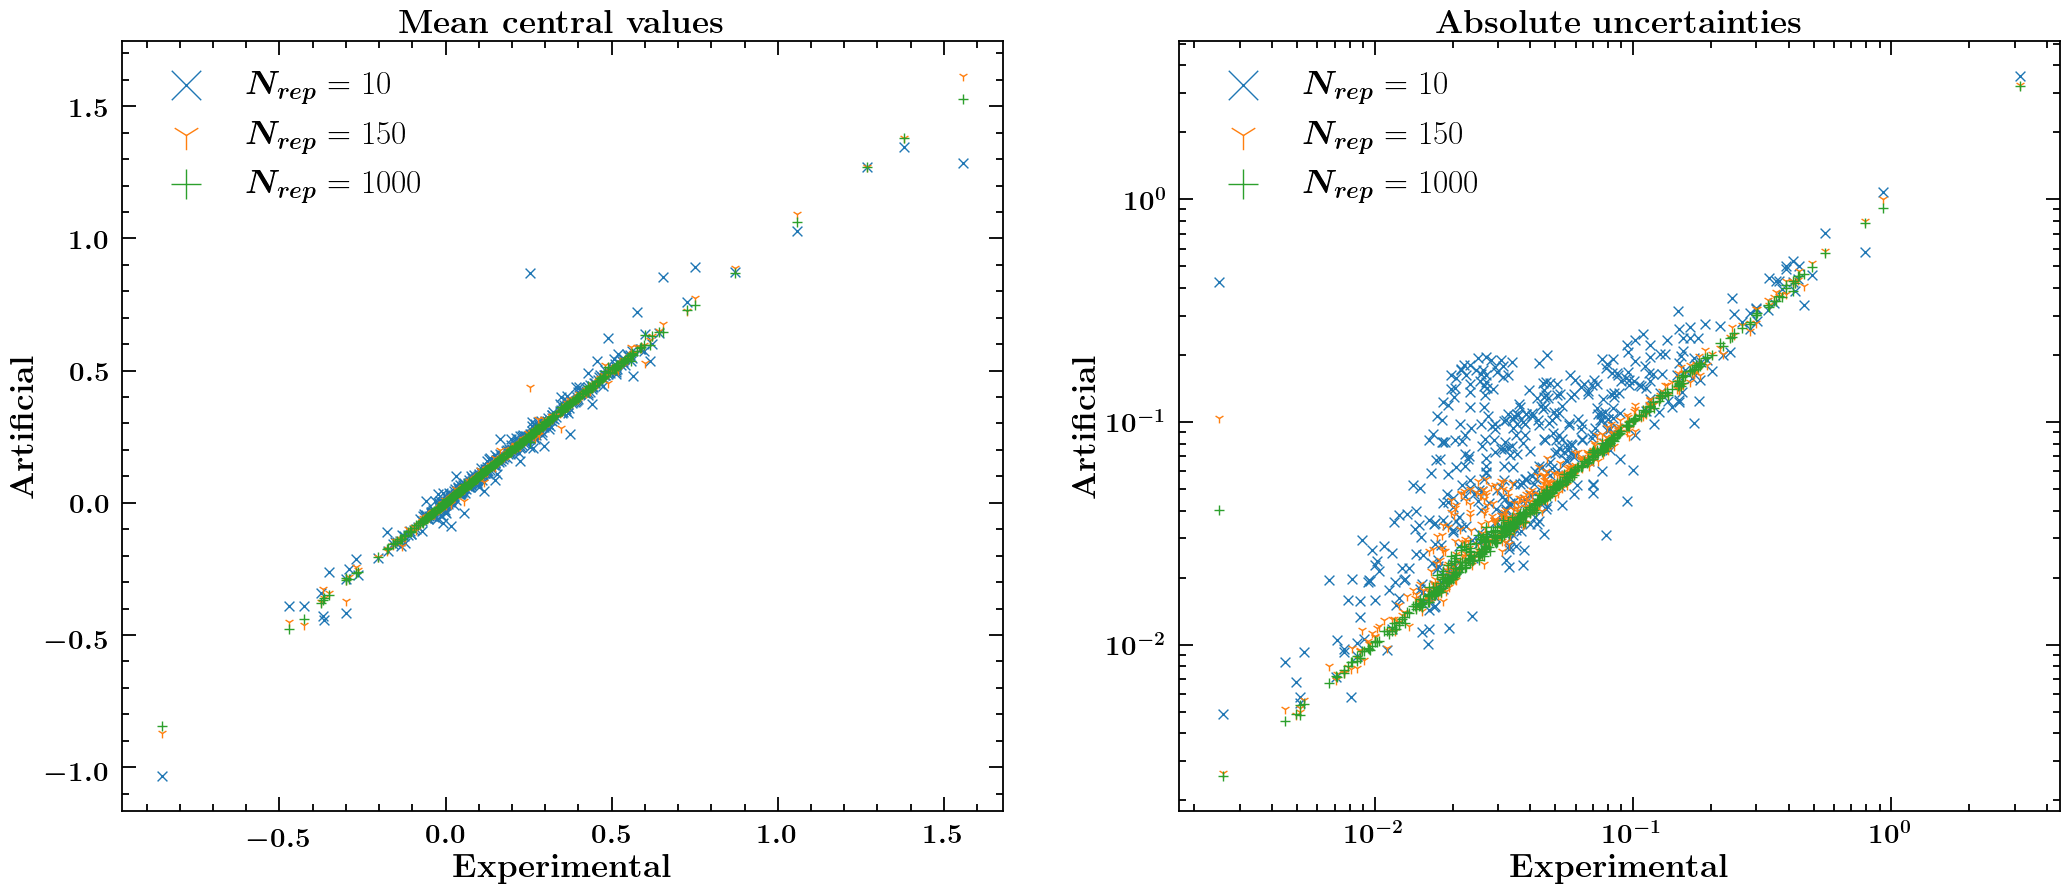
\includegraphics[width=1\textwidth]{replica_number.png } 
  \caption{\small{Scatter plot of experimental versus artificial Monte Carlo mean central values and absolute uncertainties of polarized structure functions computed from ensembles made of $N_{\T{rep}} = 10$, $100$, $1000$ replicas.}}
  \label{fig:replica_number}
\end{figure}
%%
It immediately follows that $\langle \chi^2 \rangle = N_{\T{dat}}$, as predicted by the $\chi^2$ distribution. Now, the covariance matrix, being a symmetric object, admits the so called Cholesky decomposition, that allows us to write
%%
\begin{equation}
  \vb*{V} = \vb*{L} \cdot \tran{\vb*{L}} \,,
\end{equation}
%%
where $\vb*{L}$ is a lower diagonal matrix\footnote{Further details on the Cholesky decomposition can be found in Appendix \ref{app:lin_sys}.}. Thus, the $\chi^2$ in Eq.~\eqref{eq:chi_fluc} can be recast as
%%
\begin{equation}
  \chi^2 = \left| \vb*{L}^{-1} \cdot \vb*{d} \right|^2 \,.
  \label{eq:chi2_Cholesky}
\end{equation}
%%
Collecting Eqs.~\eqref{eq:chi2_Cholesky} and \eqref{eq:chi2_normal} and after a little algebra, one finally obtains the following relation
%%
\begin{equation}
  f_j = m_j + \sum_{i=1}^{N_{\T{dat}}} L_{ji} z_i\,.
  \label{eq:MC_gen}
\end{equation}
%%
We stress that the above expression has been obtained by imposing that the fluctuated data followed the multi-variate Gaussian distribution and that the $\chi^2$ had the correct distribution. Thus, in order to generate an artificial value, one just has to use Eq.~\eqref{eq:MC_gen}, where $z_j$ is randomly extracted from a centred, univariate Gaussian distribution.\par
It is straightforward to show that the fluctuations generated according to Eq.~\eqref{eq:MC_gen} present the same statistical properties of the original data set. In particular, one can show that
%%
\begin{gather}
  \langle f_j \rangle = m_j \,,\\
  \langle f_j f_k \rangle = \langle f_j \rangle \langle f_k \rangle + V_{jk} \,,
\end{gather}
%%
which are the expected relations for a correct generation of a Monte Carlo ensemble.\par
The number of replicas is chosen in order to faithfully reproduce the statistical estimators of the original experimental data. For instance, we can check if the averages and the variances of the replica sample, that is
%%
\begin{equation}
  \langle F_{i}^{\T{(art)}} \rangle = \frac{1}{N_{\T{rep}}} \sum_{k=1}^{N_{\T{rep}}} F_{i}^{(k)} \hspace{5mm} \T{and} \hspace*{5mm} \sigma_i^{\T{(art)}} = \sqrt{ \langle \left( F_{i}^{\T{(art)}} \right) \rangle - \langle F_{i}^{\T{(art)}} \rangle^2} \,,
\end{equation}
%%
reproduce the experimental central values and the uncertainties. Such a comparison is shown in Fig.~\ref{fig:replica_number}, where we display scatter plots of the central values and errors for sample of $N_{\T{rep}} = 10$, $150$ and $1000$ replicas. Although they only provide a qualitative description, they clearly show that the accuracy of the sample increases with the size of the Monte Carlo sample. A more quantitative description can be carried out by defining appropriate statistical estimators. Following Ref.~\cite{DelDebbio:2004xtd}, we use the percentage error and the scatter correlation r for central values, whose definitions are
%
\begin{gather}
  \left< PE \left[ \left< F^{(\T{art})} \right>_{\T{rep}} \right] \right>_{\T{dat}} = \frac{1}{N_{\T{dat}}} \sum_{i=1}^{N_{\T{dat}}} \frac{\abs{\left< F_i^{\T{(art)}} \right>_{\T{rep}} - F_{i}^{\T{(exp)}}}}{F_i^{\T{(exp)}}}\,, \\
  %%
  r \left[ F^{\T{(art)}} \right] = \frac{\left< F^{\T{(exp)}} \left< F^{\T{(art)}} \right>_{\T{rep}} \right>_{\T{dat}} - \left< F^{\T{(exp)}} \right>_{\T{dat}} \left<  \left< F^{\T{(art)}} \right>_{\T{(rep)}}\right>_{\T{dat}} }{\sigma_s^{\T{(exp)}} \sigma_s^{\T{(art)}} }\,,
\end{gather}
%%
where the scatter variance are defined as
%%
\begin{gather}
  \sigma^{\T{(exp)}}_s = \sqrt{\left< \left( F^{\T{(exp)}} \right)^2 \right>_{\T{dat}} - \left( \left< F^{\T{(exp)}} \right>_{\T{dat}} \right)^2} \,,\\
  %
  \sigma^{\T{art}}_s = \sqrt{\left< \left( \left<F^{\T{(art)}}\right>_{\T{rep}} \right)^2 \right>_{\T{dat}} - \left( \left< \left<F^{\T{(art)}}\right>_{\T{rep}} \right>_{\T{(dat)}} \right)^2} \,.
\end{gather}
%%
Essentially, the percentage error describes how well the central values are recovered by the Monte Carlo sample. On the other hand, the scatter correlation $r$ reflects the capacity of the Monte Carlo sample to reproduce the correlations that are present in the original data set. For each experiment, we show these two values for the observables $g_1^{(h)}$ and $g_1^{(h)}/F_1^{(h)}$ in Tab.~. We see that a Monte Carlo sample with size $N_{\T{rep}} = 150$ gives a satisfactory reproduction of mean values and uncertainties of experimental data. The improvements obtained by using a larger sample are moderate, and, in any case, do not justify the higher computational effort. For these reasons, we will henceforth adopt the ensemble with $N_{\T{rep}} = 150$ replicas as the standard configuration for our fits.

\section{Details of the analysis}
\label{sec:4.2}
Here we summarise the aspects concerning the QCD analysis of polarised structure functions. The main observables throughout the analysis are the structure functions $g_1$, Eq.~\eqref{eq:g1_QFT}, and $g_1^h$, Eq.~\eqref{eq:g1h}, for DIS and SIDIS respectively. They are expressed in terms of combinations of PDFs and provide complementary constraints on the distributions.%

On the one hand, data coming from DIS experiments constraints only the linear combination of $\Delta \Sigma$, $\Delta T_3$, $\Delta T_8$, together with $\Delta g$, as it can be easily seen from Eq.~\eqref{eq:g1_NPM_ev}. On the other hand, SIDIS data provides full flavour separation. Moreover, given that data with kaons in the final state are given, the constraining power for the strange distributions $\Delta s$ and $\Delta \bar{s}$ is strengthened. In both SIDIS and DIS processes, the gluon distribution $\Delta g$ is weakly constrained. Indeed, it enters at NLO and its effect is lessened by the running coupling. Processes other than those we have just discussed (such as jet or semi-inclusive production in proton-proton collisions), receiving LO contributions from gluon initiated subprocesses, may provide direct information on the gluon distribution \cite{Rojo:2015acz}.%

Since we use data with different targets, we must take into account the hadron that PDFs refer to. The proton, neutron, and deuteron PDFs are related to each other by isoscalarity (assumed as an exact symmetry) so that
%%
\begin{equation}
  \begin{split}
    &\Delta u^{(I)} = I \Delta u^p + ( 1 - I ) \Delta d^p \\
    &\Delta d^{(I)} = I \Delta d^p + ( 1 - I ) \Delta u^p
  \end{split}
  \label{eq:iso_rel}
\end{equation}
%%
where $I=1$, $0.5$ and $0$ representing proton, deuteron, and neutron respectively. A similar relation also holds for antiquark distributions. We will henceforth assume that PDFs refer to the proton. The other distributions can be obtained by means of Eqs.~\eqref{eq:iso_rel}.%

Since both $\Delta s$ and $\Delta \bar{s}$ are sea-distributions for all targets, we will further assume that
%%
\begin{equation}
  \Delta s = \Delta \bar{s} \,.
\end{equation}
%%
In doing so, we decrease the number of unknown quantities, and focus the analysis to valence quarks. We will also neglect the heavier quark and antiquark distributions for charm and bottom flavours. The threshold under which this assumption is reliable has been fixed to the quark masses, assuming the values $m_c=1.51\, \T{GeV}$ and $m_b=4.92\, \T{GeV}$. For the QCD calculation, the value for the strong coupling constant has been fixed to $\alpha_s(M_Z^2) = 0.118$.\par
Finally, the computation of SIDIS observables requires the introduction of fragmentation functions sets. For this analysis, we will use the pion and kaon fragmentation functions sets \texttt{MAPFF1.0} obtained from a global analysis carried out at next-to-next-to-leading order \cite{Khalek:2021gxf, AbdulKhalek:2022laj}.

\section{Fitting configuration}
\label{sec:4.3}
In this section, we shall give the details of the fitting configuration adopted in the \texttt{MAPPol1.0} analysis. We discuss which flavours are taken into account and how the distributions are parametrised in terms of neural network. Then, we will move to the description of the training procedure, providing a more detailed picture than that given in \secref{sec:NNtr}. In particular, we will see the difference between the error function used during the minimisation and the global error function. Finally, we review the theoretical constraints assumed in the analysis and their implications.

\subsection*{Neural Network parametrisation}
The six independent distributions that are of our concern throughout the analysis are $\Delta u, \, \Delta d, \, \Delta s, \, \Delta \bar{u}, \, \Delta \bar{d}$ and $\Delta g$. These distributions are parametrised in terms of a single multi-layer feed-forward neural network, whose output layer is compounded of six differential nodes, one for each distribution. The PDFs are intended to be parametrised at an initial scale $\mu_0 = 1 \, \T{GeV}$. The output of the network is then evolved to the experimental scale by means of the DGLAP equations, Eq.~\eqref{eq:DGLAP_coupled}.%

The architecture of the neural network is 1-10-6, which entails 86 free parameters. We explicitly verified the parametrisation to be redundant, ensuring that the results do not depend on the architecture. Indeed, keeping on the single deep-layer structure, we have not observed any considerable differences in the results by either improving the nodes of the internal layer up to 20 or reducing this number to 5. We figured out that an architecture with 10 internal nodes is a good compromise between the number of parameters and the redundancy in the parametrisation, which is enough to reproduce any functional form given sufficient training time.%

The single node in the input layer corresponds to the Bjorken variable $x$. Other determinations supplement the above parametrisation with a preprocessing function. This consists of multiplying the neural network by a fixed function that reflects some known behaviour of the distributions. For instance, the \texttt{NNODFpol1.0} analysis from NNPDF collaboration \cite{Nocera:2014gqa} introduces these functions to implement small- and large-x behaviours of the distributions. Even though such an approach may help the algorithm in terms of efficiency, it can be source of biases. For that reason, we choose to use the neural network without any preprocessing function.%

All the nodes except for the input node use a sigmoid as activation function, Eq.~\eqref{eq:sigmoid}. However, we slightly modify the outputs of the last node in order to constraint to zero parton distributions at $x=1$ and to implement, analytically, theoretical constraints, as we shall see later.%

Finally, we remark that there are as many networks as the number of replicas that we are working with. In our case, we will deal with 150 neural networks, representing the statistical ensemble of polarised PDFs. Since dealing with such a huge number of networks is a heavy computational task, the outputs (\textit{i.e.}, the PDFs) are put on a grid in the $(x,Q^2)$ plane. The value for an arbitrary pair $(x,Q^2)$ can be easily accessed through the LHAPDF interface \cite{Buckley:2014ana}. A schematic representation of the neural network and of the subsequent steps is sketched in Fig.~\ref{fig:NN_plot}.
%%
\begin{figure}[t]
  \centering
  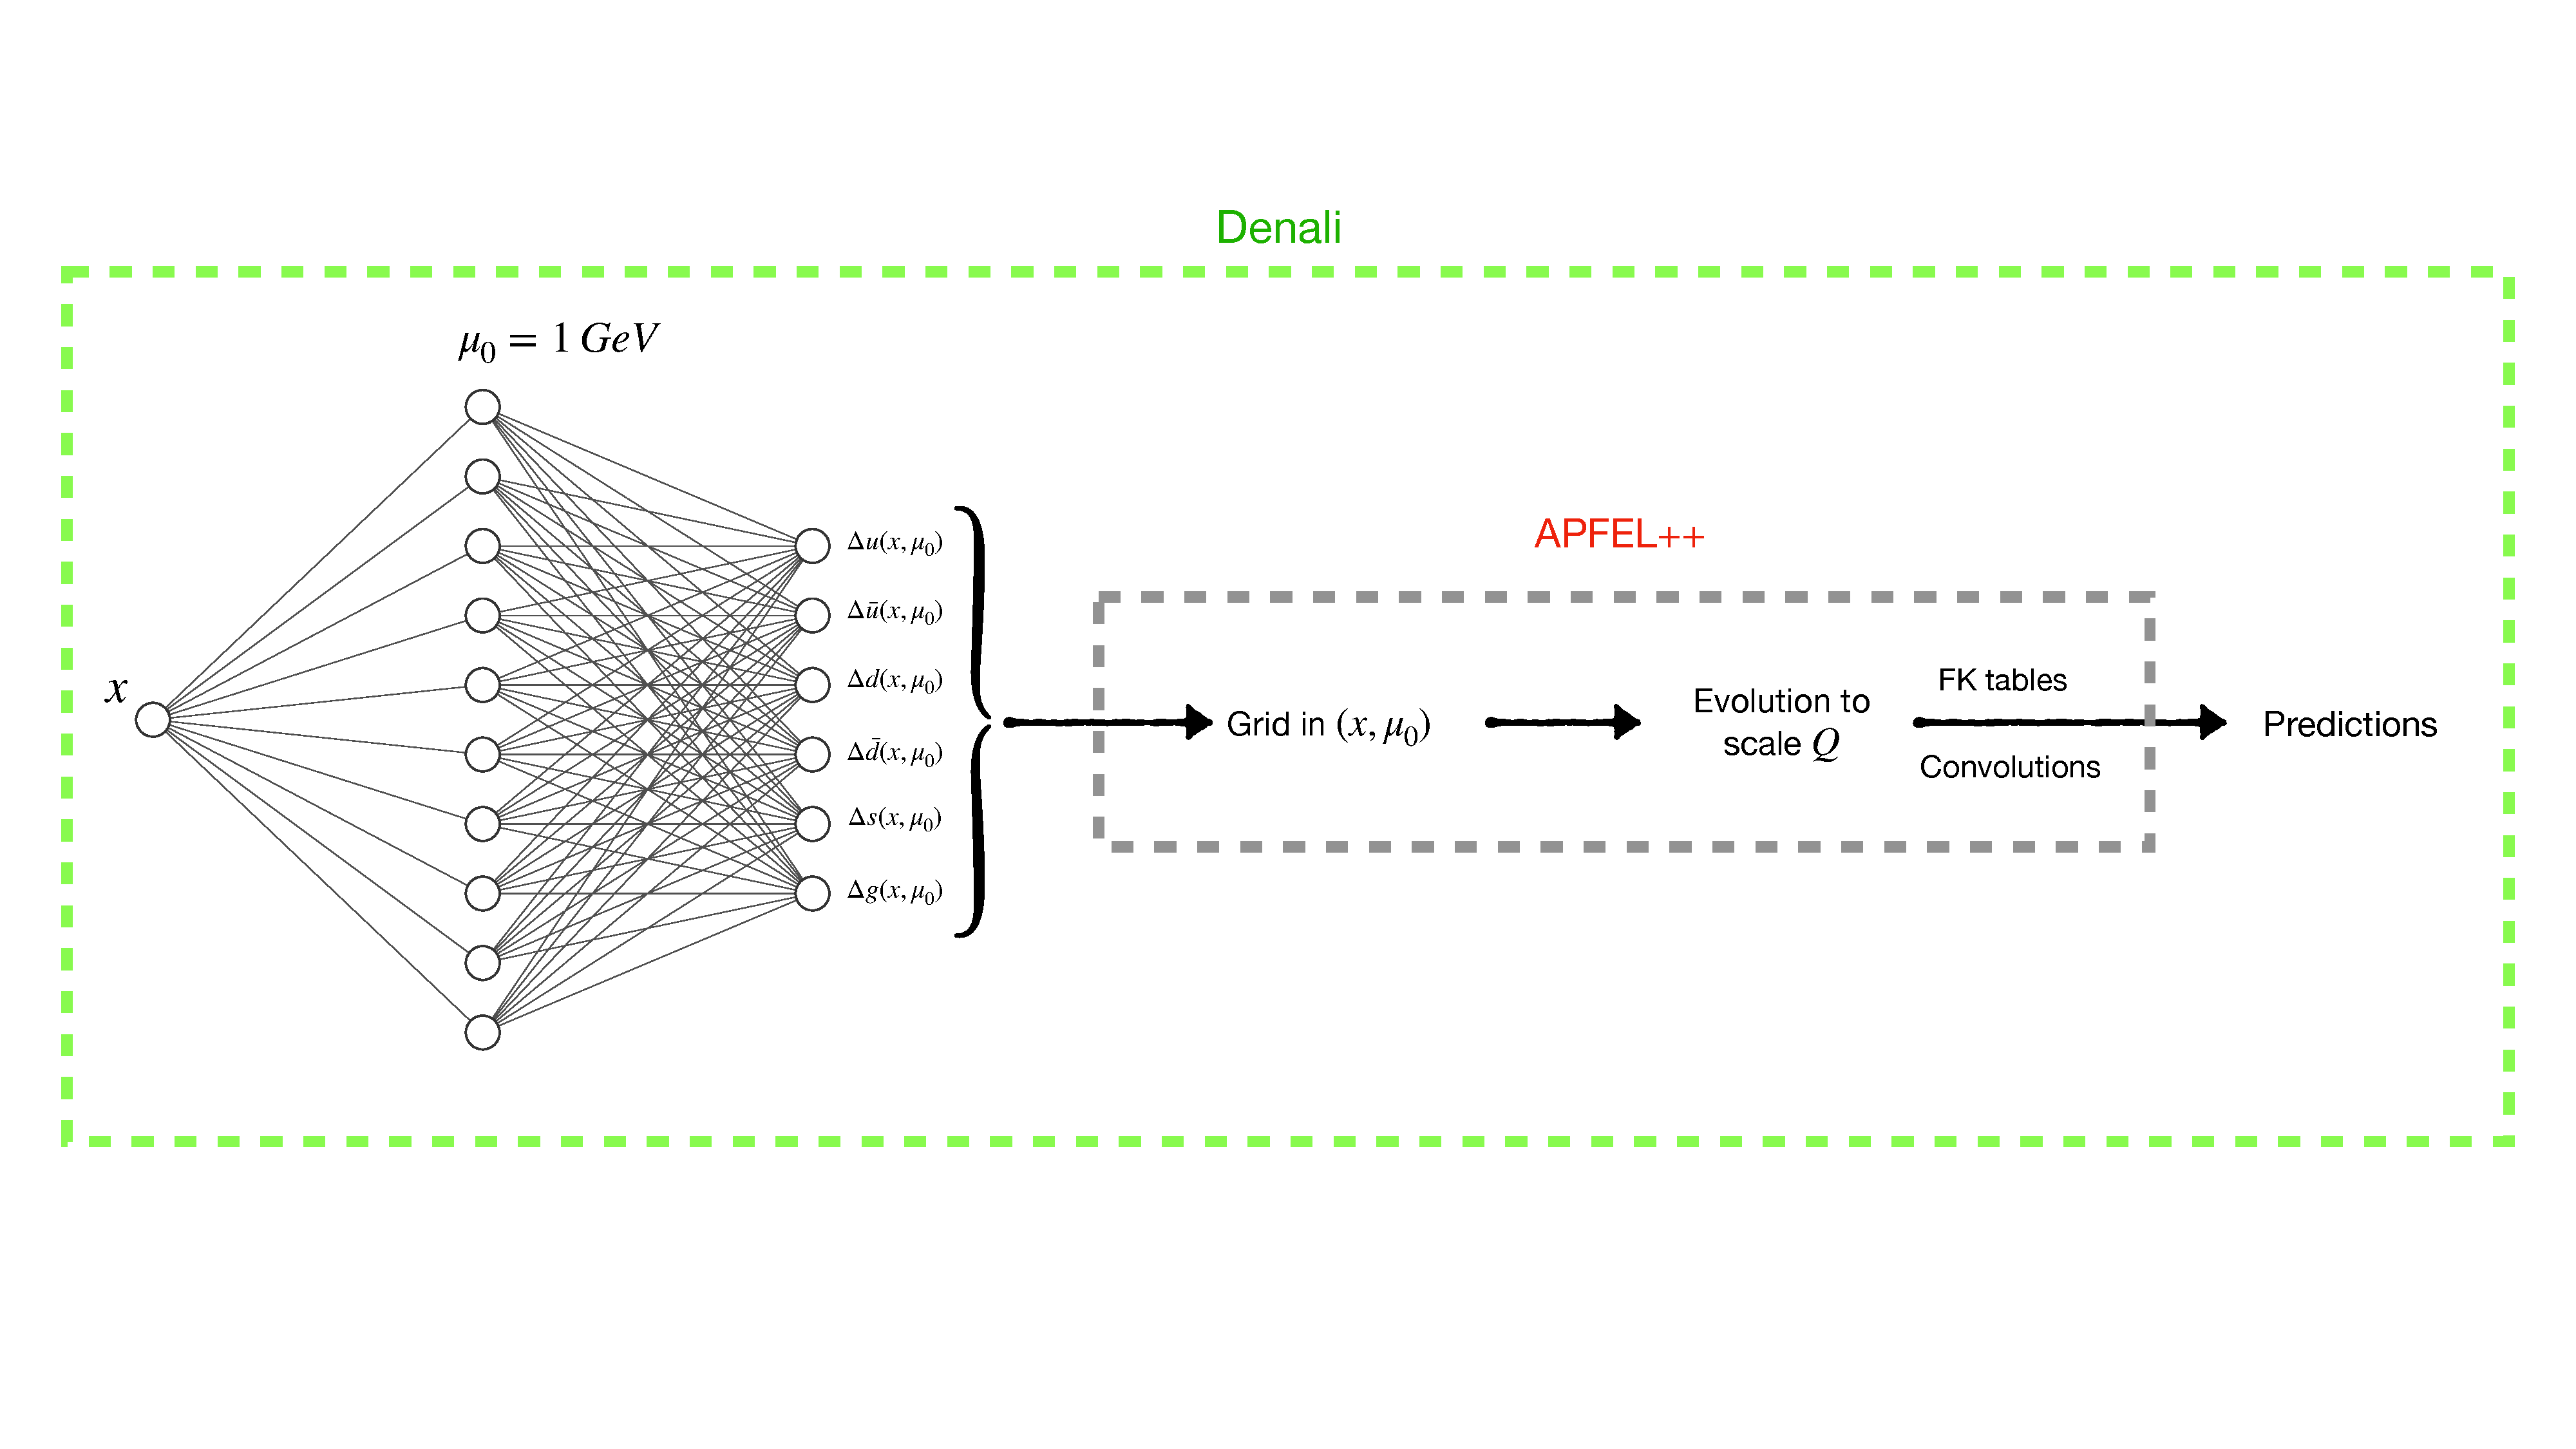
\includegraphics[width=1\textwidth]{NN_plot.pdf} 
  \caption{\small{Scheme of the \texttt{Denali} algorithm.}}
  \label{fig:NN_plot}
\end{figure}
%%

\subsection*{Optimization and determination of the optimal fit}
Optimization is the process where the parameters are optimised through the minimisation of the figure of merit over the parameter space. Each replica of the ensemble (\textit{i.e.}, each network) undergoes an independent optimisation procedure. Although this process can be computationally expensive if a high number of replicas is used, we can use parallel processing methods, and the time required by a single global fit is considerably reduced.%

The figure of merit for the $k$-th replica is defined as
%%
\begin{equation}
  E^{(k)} = \frac{1}{N_{\T{dat}}} \sum_{i,j}^{N_{\T{dat}}} \left( g_{i}^{\T{(art)}(k)} - g_{i}^{\T{(net)}(k)} \right) (\T{cov})^{-1}_{ij} \left( g_{j}^{\T{(art)}(k)} - g_{j}^{\T{(net)}(k)} \right) \,.
  \label{eq:EF_k}
\end{equation}
%%
The above expression requires few comments. The observable $g_{i}^{\T{(art)}(k)}$ is the $k$-th Monte Carlo replica of the $i$-th data point, whereas $g_{i}^{(net)(k)}$ is its prediction provided by the $k$-th neural network representing the $k$-th replica of the PDF ensemble. Finally, $\T{(cov)}$ is the usual covariance matrix constructed from the experimental sets.%

The error function, Eq.~\eqref{eq:EF_k}, must not be confused with the $\chi^2$ used to quantify the goodness of the final result. Indeed, it can be shown that Eq.~\eqref{eq:EF_k} does converge to $2$ instead of $1$. The reason being that the prediction is compared against the fluctuated data and not against the experimental central value. The quantity we should refer to as the $\chi^2$ involves 
experimental central value and is defined as
%%
\begin{equation}
  \chi^2 = \frac{1}{N_{\T{dat}}} \sum_{i,j}^{N_{\T{dat}}} \left( F_{i}^{\T{(exp)}} - \left<F_{i}^{\T{(net)}}\right>_{\T{rep}} \right) (\T{cov})^{-1}_{ij} \left( F_{j}^{\T{(art)}} - \left<F_{j}^{\T{(net)}}\right>_{\T{rep}} \right) \,,
  \label{eq:global_chi2}
\end{equation}
%%
where the average over replicas is defined as
%%
\begin{equation}
  \left< F_i^{\T{(net)}} \right>_{\T{rep}} = \frac{1}{N_{\T{rep}}} \sum_{k} F^{(k)}_i \,.
\end{equation}
%%
Here, $F_i$ may represent one of the observable presented in Tab.. We will refer to Eq.~\eqref{eq:global_chi2} as the global $\chi^2$. It is computed at the end of the optimisation procedure and thus it is not minimised. The parameter space is explored with the SGD method discussed in \secref{sec:NNtr}, which sought for the minimum of the error function, Eq.~\eqref{eq:EF_k}.%

As discussed at the end of \secref{sec:NNtr}, the neural network parametrisation is able to fit not only the underlying physics, but also statistical noise of the data set -- a problem also known as \textit{overlearning}. Thus, the best fit does not always coincide with the minimum of the figure of merit, Eq.~\eqref{eq:EF_k}. In order to find the best fit, we use the cross-validation method \cite{pml1Book}. It works as follows:
%%
\begin{enumerate}
  \item For each replica, the data sets are randomly divided into two sets -- training and validation sets. They include a fraction $f_{\T{tr}}$ and $f_{\T{val}} = 1 - f_{\T{tr}}$ of the data points, respectively.
  \item During the optimisation procedure, the error function, Eq.~\eqref{eq:EF_k}, is separately computed over the training and the validation set. The former undergoes the minimisation procedure, while the latter is only monitored and not minimised.
  \item Finally, the best fit corresponds to the minimum of the validation's error function within a fixed number of iterations, which in our case corresponds to $N_{\T{iter}} = 3000$.
\end{enumerate}
%%
The profile of the figure of merit for an arbitrary replica is shown in Fig.~\ref{fig:profile}. We see that immediately after the minimum of the validation curve has been reached, it starts to increase, whereas the training curve keeps reducing. This means that the network is learning the statistical noise of the training set, which is different from that of the validation set. In the present analysis, equal training and validation fractions are chosen, that is $f_{\T{tr}} = f_{\T{val}} = 50\%$. However, some experimental sets are highly affected by the kinematic cuts and only a small portion of data points survives. In this case, the training set would be too small, affecting the stability of the minimisation. Hence, if the number of points after cuts is less or equal to 5, all the points will be included in the training set.

%%
\begin{figure}[t]
  \centering
  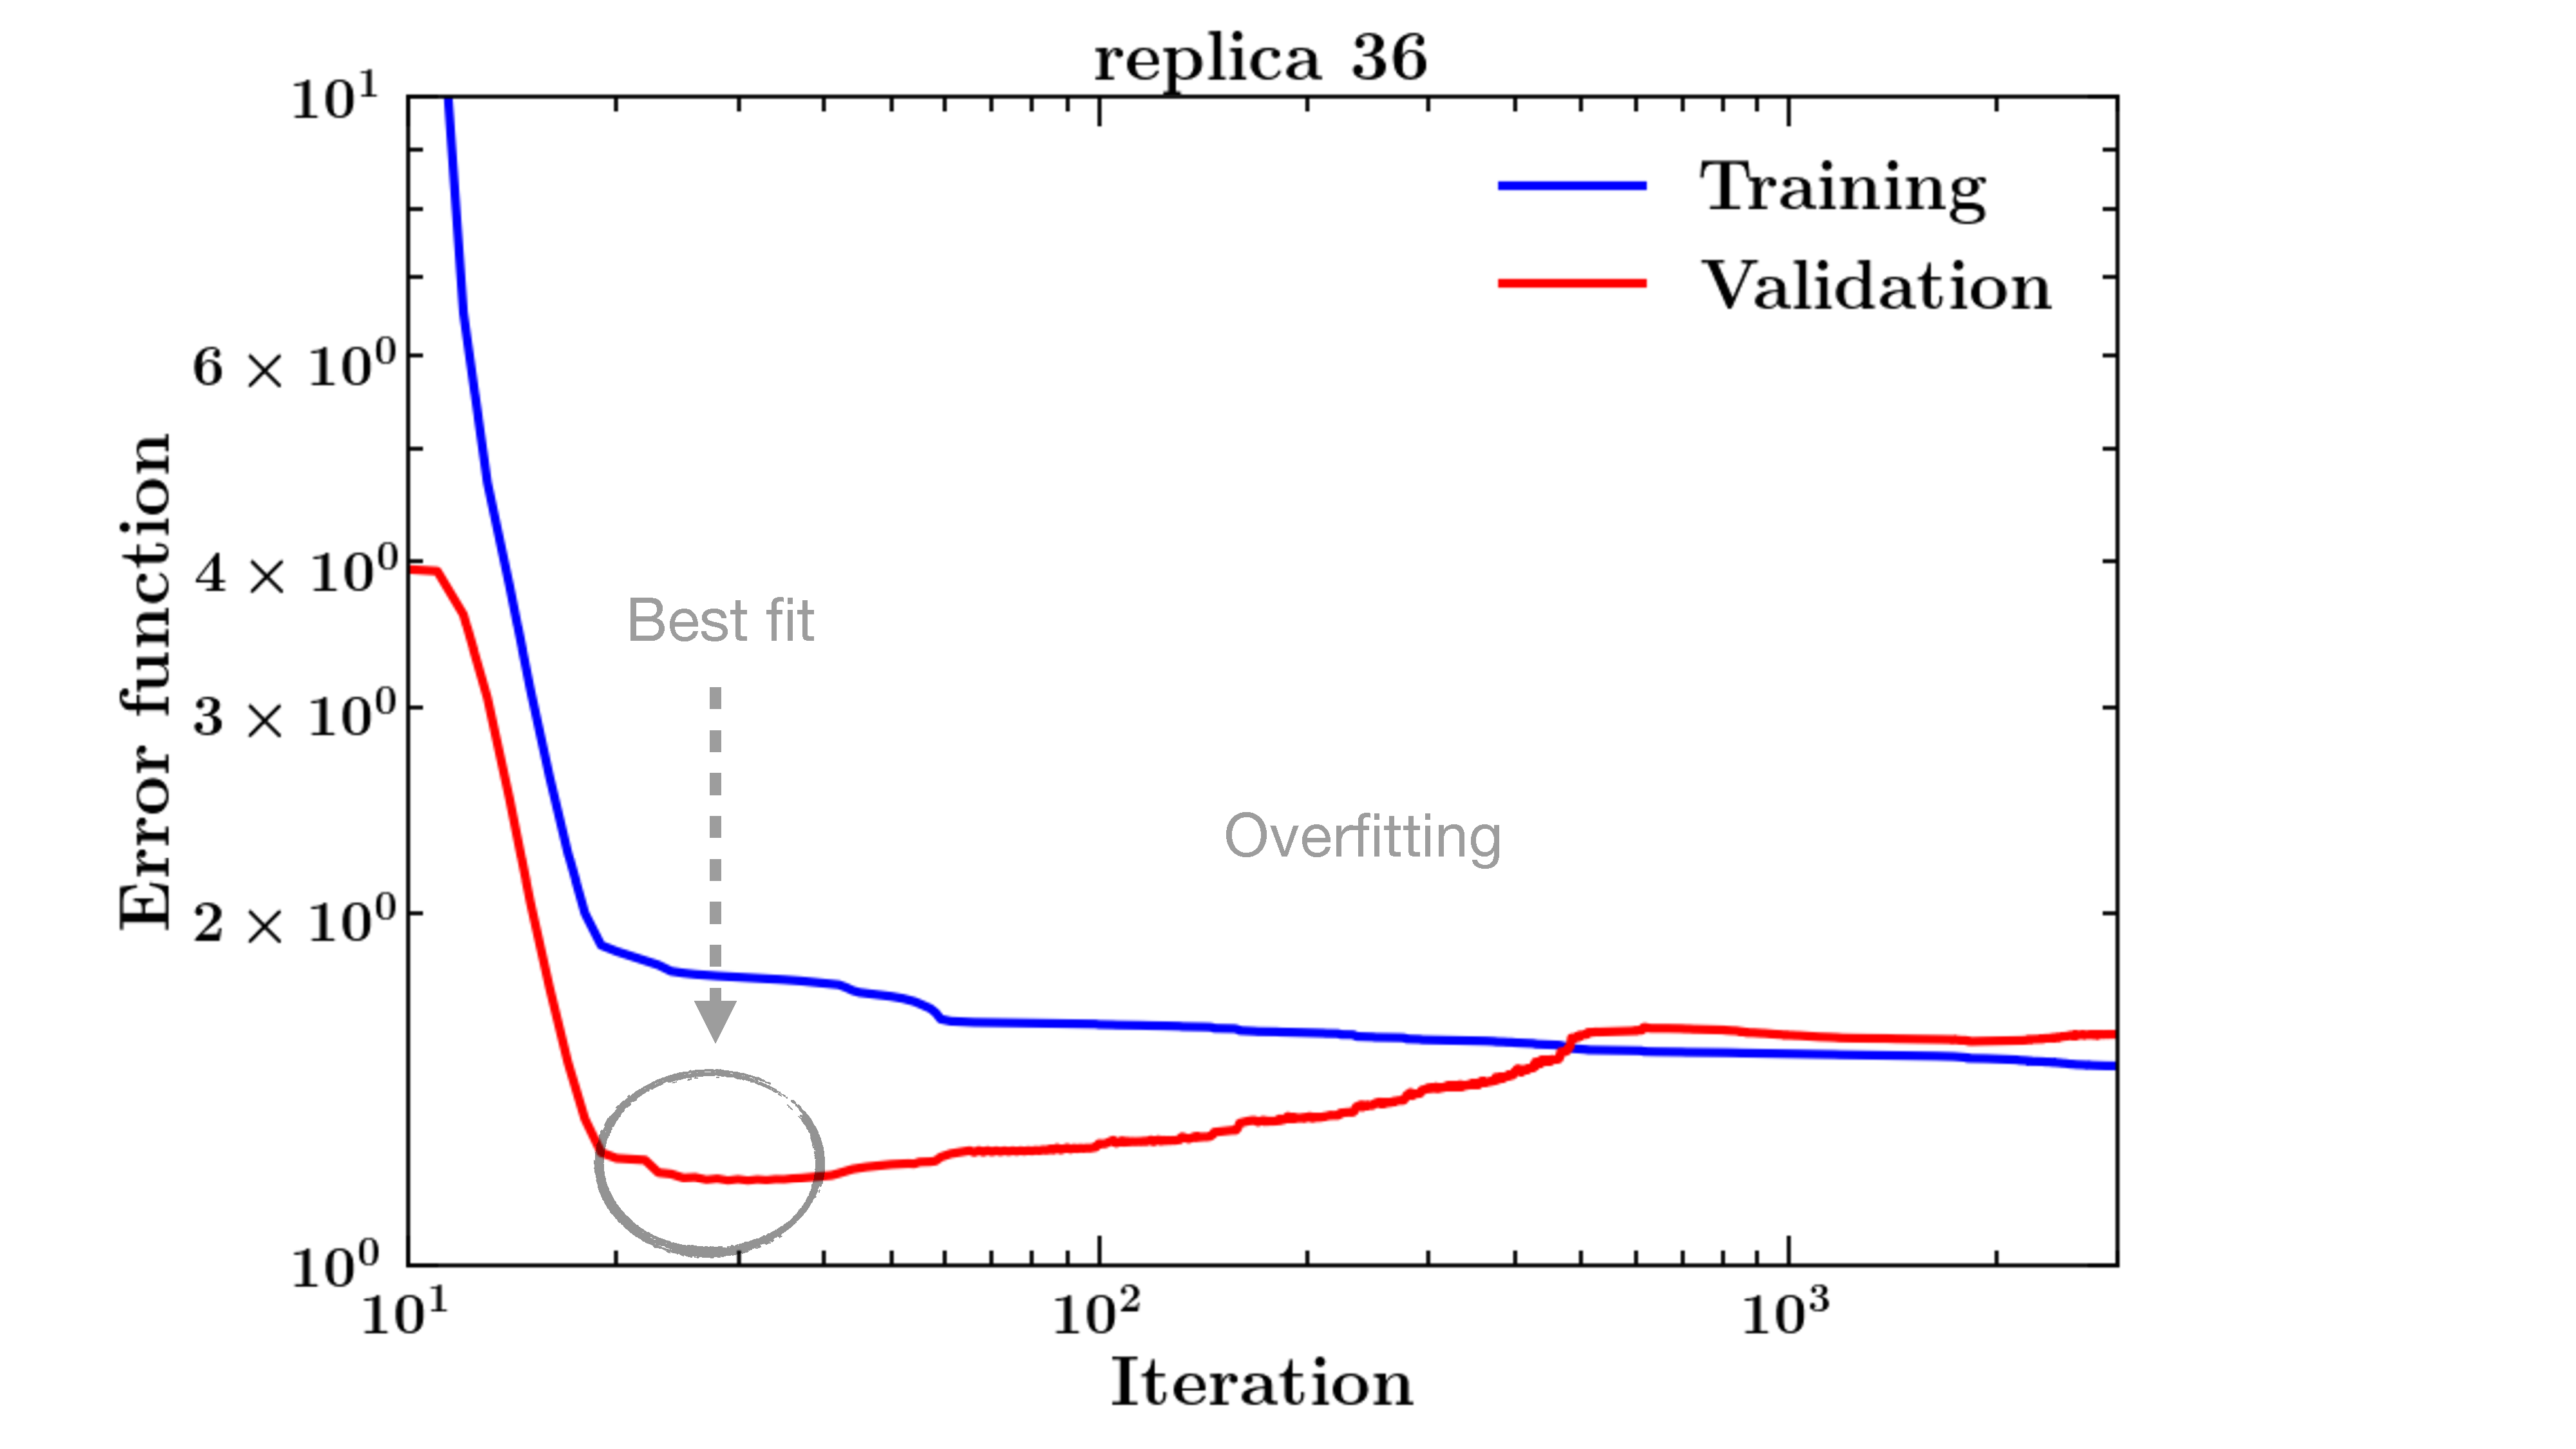
\includegraphics[width=0.6\textwidth]{profile.pdf} 
  \caption{\small{Profile of the error function for the 36th replica. The blue and red curves represent the error as a function of the iteration step for the training and validation steps, respectively.}}
  \label{fig:profile}
\end{figure}
%%

\subsection*{Theoretical constraints}
We have already mentioned that, due to the scarcity and the low accuracy of data, polarised PDF are loosely constrained. This not only affects the efficiency of the algorithm, but has a huge impact on the final result. In order to improve the constraining power and to reduce the uncertainties of the polarised PDFs, we apply theoretical constraints to the analysis. In particular, we consider sum rules and positivity.%

Sum rules refer to the hadronic matrix elements $a_3$ an $a_8$, whose values can be extracted from measurements in hyperon $\beta$-decay, Eqs.~\eqref{eq:a3_a8_values}. They can be related to the PDFs via Eqs.~[\ref{eq:a3_PM}-\ref{eq:a8_PM}], provided that exact $SU(3)_f$ symmetry is assumed. The theoretical constraint is introduced at a data set level. This means that the values in \eqref{eq:a3_a8_values} are treated as standard data points, with central value and (uncorrelated) uncertainty. Hence, at each iteration of the optimisation procedure, the algorithm will compute, in addition to the observable $g_1^{(h)}$ or $g_1^{(h)}/F_1^{(h)}$, the predictions for $a_3$ and $a_8$ via Eqs.~[\ref{eq:a3_PM}-\ref{eq:a8_PM}]. Sum rules provide further information on polarised PDFs. If the SIDIS data sets were not included, the only source of information for the sea-quark flavour $\Delta s$ would only come from this theoretical constraint. It will be interesting to study how these constraints affect that distribution if SIDIS data sets are excluded.%

The other theoretical constraints, which enforce the most the PDFs, is the positivity constraint. The key point is that the cross-sections that enter the polarised asymmetries, Eq.~\eqref{eq:asymmetry}, must be positive. This implies that $g_1^{(h)}$ is bounded by its unpolarised counterpart $F_1^{(h)}$, that is
%%
\begin{equation}
  \begin{split}
    \left| g_1 (x,Q^2)  \right|& \leq F_1(x, Q^2) \,,\\
    \left| g_1^{(h)} (x,z,Q^2)  \right|& \leq F_1^{(h)}(x, z, Q^2) \,.
  \end{split}
  \label{eq:positivity_obs}
\end{equation}
%%
Given that at leading order the structure function are proportional to parton distributions, and that Eq.~\eqref{eq:positivity_obs} must be satisfied for any choice of target (\textit{i.e.}, for any combination of quark plus antiquarks), it must be satisfied by each flavour separately. Hence, at leading order, we have
%%
\begin{equation}
  \left| \Delta f_i (x,Q^2) \right| \leq f_i (x,Q^2) \,,
  \label{eq:positivity_fl}
\end{equation}
%%
for all $x$ and for all $Q^2$, being $f_i$ the relative unpolarised PDF set. At NLO and beyond the positivity constraint, Eq.~\eqref{eq:positivity_fl}, receives perturbative corrections. Nevertheless, it can be shown \cite{Altarelli:1998gn} that, even at relatively small values down to $Q^2 \sim 1 \, \T{Gev}^2$, the modified positivity bounds for each flavours are slightly different from the leading order bounds, and the difference between LO and higher orders is negligible. Moreover, the positivity bound exhibits his constraining effects only at large x, where the higher order corrections to the LO positivity bound are lessened. Imposing positivity bounds consistently guarantees positivity of physical cross-sections.%

The positivity bound Eq.~\eqref{eq:positivity_fl} must take into account the uncertainties of the unpolarised PDFs. This problem can be addressed with two different solutions. The first imposes the leading-order bound Eq.~\eqref{eq:positivity_fl} by requiring
%%
\begin{equation}
  \left| \Delta f_i (x,Q^2) \right| \leq \left<f_i (x,Q^2)\right>_{\T{rep}} + \sigma_i(x,Q^2) \,,
  \label{eq:positivity_fl_sigma}
\end{equation}
%%
where $\left<f_i (x,Q^2)\right>_{\T{rep}}$ is the mean value over the statistical ensemble of unpolarised PDFs and $\sigma_i(x,Q^2)$ its corresponding one-sigma uncertainty, both evaluated at the kinematic point $(x,Q^2)$. This ensures that also the uncertainty of the unpolarised distribution is propagated through the analysis within a standard deviation. On the other hand, the second approach applies the same bound Eq.~\eqref{eq:positivity_fl}, but with randomly chosen replica from the statistical set of distributions. This means that, replica by replica, the unpolarised PDF that enters the constraint is different. Hence, this stocasticity spans the space of distributions, reflecting the uncertainties of the statistical ensemble in the bound. For consistency, the unpolarised PDF set is the same that has been used to compute the unpolarised structure function $F_1^{(h)}$. \red{Which method do we adopt?}%

The positivity constraint is introduced analytically in the present work, acting on the output layer of the neural network. Indeed, for each output node of the last layer (\textit{i.e.}, for each parametrised flavour), we impose
%%
\begin{equation}
  \sigma_{i} (x,\mu_0) \rightarrow \Delta f_{i} (x, \mu_0) \equiv \bigl[ 2 \sigma(x,\mu_0) - 1 \bigr] \, f_{i} (x,Q^2) \,,
  \label{eq:pos_net}
\end{equation}
%%
being $\sigma_i(x,\mu^2)$ the sigmoid activation function of the $i$-th output of the network. We observe that Eq.~\eqref{eq:pos_net} not only imposes the positivity bound Eq.~\eqref{eq:positivity_fl}, but also constraint to zero parton distribution at $x=1$, provided that the unpolarised PDF is zero at the same point. 


\section{Results}
\label{sec:4.4}


\chapter{Conclusions}
\label{ch:5}

Polarised parton distribution functions play a key role in the context of perturbative QCD, and enter the calculations involved in any phenomenological study of hard scattering processes with polarised hadrons in the initial state. In this Thesis, I presented the first determination of spin-dependent parton distribution functions of the proton at next-to-next-to-leading order accuracy in pQCD.%

Experimental data of polarised processes are both less abundant and less precise than those available in the unpolarised counterpart, and polarised parton distributions are then known with much less precision. However, as the quality of the experimental information improves, it becomes more and more necessary to develop a solid framework that is able to face future data and that allows for more accurate determinations. The Electron-Ion Collider, which is expected to operate in the 2030s, will increase the precision of measurements and enlarge the kinematic coverage of data, rather limited at the present as shown in \secref{sec:4.2}. On the one hand, a wider kinematic range would reduce PDF uncertainties in the extrapolation regions. On the other hand, higher precisions will require more accurate predictions, possible by increasing the perturbative order in the calculations of observables. Hence, even though providing the first determination of polarised PDFs at NNLO accuracy has been the major goal of the present Thesis, it also wishes to provide a benchmark for the suitability of the presented framework for future data. Moreover, the results presented in this Thesis may suggest the way in which future measurements should be performed at the EIC in order to increase the quality of PDF determinations.%

The analysis has been carried out within the MAP methodology, inspired by the framework developed by the NNPDF Collaboration. The statistical tools adopted in this Thesis include Monte Carlo methods for error propagation, neural network for PDF parametrisation, and stochastic gradient descent for parameter optimisation. The determination is based on available data from inclusive and semi-inclusive Deep-Inelastic Scattering. The main results presented in this Thesis are here summarised:
%
\begin{itemize}
  \item I determined the \texttt{MAPpol1.0} set of helicity-dependent PDFs at NNLO accuracy in perturbative QCD, based on inclusive and semi-inclusive DIS data. The impact of higher order corrections on valence distributions is negligible, while sea quark distributions at NNLO differ in some respects. With regard to the gluon, it also acquires small changes when extracted at NNLO, still remaining highly unconstrained by the included data. Even though the global $\chi^2$ of the NNLO fit indicates a very good agreement between predictions and data, it has been observed a deterioration of the fit quality w.r.t. the NLO fit. I showed that this degradation depends on the data sets included in the analysis, and can be due to the limited precision of polarised measurements. Nevertheless, this situation might change once EIC will provide new polarised data sets with increased kinematic coverage and accuracy.
  \item The determination has been carried out by means of two theoretical constraints - sum rules and positivity. I verified that these assumptions do not introduce theoretical biases in the analysis, and that the results remain stable upon variation of these conditions. Indeed, I showed that the functional space of PDFs allowed by data is compatible, within uncertainties, with that of the theoretical constraints.
  \item I compared the \texttt{MAPpol1.0} set at next-to-leading order accuracy with other available sets \cite{Nocera:2014gqa, Ethier:2017zbq, deFlorian:2009vb} at the same perturbative order. In general, the PDF set presented in this Thesis is compatible, within uncertainties, with the other determinations, yet some differences emerge in some respects. As extensively discussed, these are mainly due to the different experimental information and methodologies that each collaboration adopts to carry out the analysis.
\end{itemize}
%

\section{Outlook and future directions}
%
The \texttt{MAPpol1.0} polarised parton set is based on inclusive and semi-inclusive DIS measurements. Still, additional information on the spin structure of the proton can be achieved by including a range of other processes to the analysis, as frequently suggested throughout this Thesis.%

The inclusion of polarised Drell-Yan measurements may be beneficial to both precision and accuracy of quark and antiquark distributions. This would require the implementation of the theoretical framework needed to compute polarised Drell-Yan predictions in the global analysis, similar to what has been done in \chapref{ch:2} for DIS and SIDIS. Currently, NLO corrections to DY cross-sections have been computed in Refs.~\cite{Gehrmann:1997ez,Bonvini:2010tp}, while at NNLO they have been recently computed in Ref.~\cite{Boughezal:2021wjw}. Alternatively, polarised Drell-Yan can be taken into account by means of the Bayesian reweighting and unweighting method \cite{Ball:2010gb, Ball:2011gg}, as done in \texttt{NNPDFpol1.1}.%

In addition, jet production from proton-proton collisions would constrain the gluon distribution at leading order thanks to gluon-initiated processes. Jet production data can be implemented only through Bayesian reweighting (as in \texttt{NNPDFpol1.1}) in a NNLO analysis, since perturbative corrections for such a process are only known at NLO~\cite{deFlorian:1998qp}.%

In conclusion, all these further constraints can be implemented in the analysis presented in this Thesis to achieve a more comprehensive scenario that includes most of the experimental information currently available. In the long term, EIC data are expected to reduce the discrepancy between polarised and unpolarised data, and thus allowing for a more reliable determination of spin-dependent parton distribution functions.


\appendix
\numberwithin{equation}{section}
\setcounter{equation}{0}
%\chapter{Spin}
\label{app:spin}

%___________________________________________________________
\section{Spin operator}
From eqs. we can extract the third component of the angular momentum\footnote{Here I am using the Weyl (chiral) basis for the Dirac matrices
\begin{equation*}
    \gamma^0 = \begin{pmatrix}
        0 & I_2\\
        I_2 & 0
    \end{pmatrix} \, , 
    \hspace{3mm}
    \gamma^k = \begin{pmatrix}
        0 & \sigma^k\\
    -\sigma^{k} & 0
    \end{pmatrix} \, ,
    \hspace{3mm}
    \gamma^5 = \begin{pmatrix}
        -I_2 & 0\\
        0 & I_2
    \end{pmatrix}\,.
\end{equation*}
}
\\
\begin{equation}
    S_z = \frac{1}{2} \sigma^{12} = \frac{i}{4} \commutator{\gamma^1}{\gamma^2} = \frac{i}{2} \gamma^1 \gamma^2 = 
    \begin{pmatrix}
        \frac{1}{2} \sigma_3 & 0 \\
        0 & -\frac{1}{2} \sigma_3
    \end{pmatrix} \,.
\end{equation}
\\
In the inertial frame of a massive particle, this operator represents the intrinsic spin\footnote{We are assuming that the quantization axis corresponds to the z-axis of the reference frame in which the particle is at rest.}. Indeed, it can be used to label Dirac states according to their spin
\\
\begin{equation}
    \begin{split}
        S_z \, u_{\pm}(\vb*{0}) = \pm \frac{1}{2} u_{\pm}(\vb*{0})\, ,\\
        S_z \, v_{\pm}(\vb*{0}) = \mp \frac{1}{2} v_{\pm}(\vb*{0})\, ,
    \end{split}
    \label{eq:spin_dirac}
\end{equation}
\\
where $u_{\pm}$ and $v_{\pm}$ obey the equations
\\
\begin{equation}
    \begin{split}
        &(\slashed{p} - m) u_s(\vb{p}) = 0 \, ,\\
        &(\slashed{p} + m) v_s(\vb{p}) = 0.
    \end{split}
    \label{eq:Dirac_eqs}
\end{equation}
\\
We can define a set of projection operators that select the spin component $s$ along the direction individuated by the z-axis
\\
\begin{equation}
    \begin{split}
        &\frac{1}{2} \qty(1 + 2 s S_z) u_{s'}(\vb*{0}) = \delta_{ss'}u_{s'}(\vb*{0}) \\
        &\frac{1}{2} \qty(1 - 2 s S_z) v_{s'}(\vb*{0}) = \delta_{ss'}v_{s'}(\vb*{0}) \,,
    \end{split}
    \label{eq:projectors}
\end{equation}
\\
provided that $s,s' \in \qty{\pm 1}$. We need to boost these operators in a general reference frame. To do so, we can try to factor out the covariance form in the rest frame. Once expressed in that form, the relation holds in any reference frame, providing the general expression for \eqref{eq:projectors}. We start by noting that, in chiral basis, we can write
\\
\begin{equation}
    S_z = \frac{i}{2}\gamma_1 \gamma_2 = -\frac{1}{2}\gamma_5 \gamma^3 \gamma^0 \,.
\end{equation}
\\
In the rest frame $\slashed{p} = \gamma^0 m$ so that we can write $\gamma^0 = \slashed{p}/m$. Moreover, if we define the four-vector $ z^{\mu} = \qty(0, \hat{z})$ then $\gamma^3 = \slashed{z}$ and the spin operator reads
\\
\begin{equation}
    S_z = -\frac{1}{2} \gamma_5 \slashed{z} \frac{\slashed{p}}{m} \,.
\end{equation}  
\\
Note that, in any frame, we have
\\
\begin{equation}
    z^2 = -1 \hspace{5mm} \textrm{and} \hspace{5mm} z \cdot p = 0 \,.
\end{equation}
\\
We can now boost in any reference frame by replacing $\slashed{z}$ and $\slashed{p}$ with their values in the frame of interest. By introducing the spin-vector $s^{\mu} = s z^{\mu}$, the projectors in eqs. \eqref{eq:projectors} can finally be written, in any reference frame, as
\\
\begin{equation}
    \begin{split}
        &\frac{1}{2} \qty(1 - 2 \frac{1}{2m}\gamma_5 \slashed{s} \slashed{p}) u_{s'}(\vb*{p}) = \frac{1}{2} \qty(1 - \gamma_5  \slashed{s}) u_{s'}(\vb*{p}) = \delta_{ss'}u_{s'}(\vb*{p})\\
        &\frac{1}{2} \qty(1 + 2 \frac{1}{2m}\gamma_5 \slashed{s} \slashed{p}) v_{s'}(\vb*{p}) = \frac{1}{2} \qty(1 - \gamma_5  \slashed{s}) v_{s'}(\vb*{p}) = \delta_{ss'}v_{s'}(\vb*{p}) \, ,
    \end{split}
    \label{eq:proj_adv}
\end{equation}
\\
where in the second equality of both equations I used eqs. \eqref{eq:Dirac_eqs} to simplify $\slashed{p}$. Now we are able to the select a single spin component from the spin sums 
\\
\begin{equation}
    \begin{split}
        &\sum_{s=\pm} u_{s} \qty(\vb{p}) \bar{u}_{s} \qty(\vb{p}) = \qty(\slashed{p} + m)\\
        &\sum_{s=\pm} v_{s} \qty(\vb{p}) \bar{v}_{s} \qty(\vb{p}) = \qty(\slashed{p} - m) \, ,
    \end{split}
\end{equation}
\\
by acting with the operators eqs. \eqref{eq:proj_adv}
\\
\begin{equation}
    \begin{split}
        &u_{s} \qty(\vb{p}) \bar{u}_{s} \qty(\vb{p}) = \frac{1}{2} \qty(1 - \gamma_5  \slashed{s}) \qty(\slashed{p} + m)\\
        &v_{s} \qty(\vb{p}) \bar{v}_{s} \qty(\vb{p}) = \frac{1}{2} \qty(1 - \gamma_5  \slashed{s}) \qty(\slashed{p} - m) \,.
    \end{split}
    \label{eq:spin:projectors}
\end{equation}

\subsection*{Relativistic limit}
Let us consider the three-momentum to be aligned in the z-direction, that is parallel to the spin quantization axis. In this reference frame we have 
\\
\begin{equation}
    \begin{split}
        &p^{\mu} = m \qty(\cosh \eta,0,0,\sinh \eta) \\
        &z^{\mu} = \qty(\sinh \eta,0,0, -\cosh \eta)\,,
    \end{split}
    \label{eq:PeZ}
\end{equation}
\\
where $\eta$ is the rapidity and the components of $z^{\mu}$ are obtained imposing $z \cdot p = 0$. In the relativistic limit ($\beta \rightarrow \pm 1$, $\eta \rightarrow \pm \infty$) the two four-vectors in \eqref{eq:PeZ} can be related as
\\
\begin{equation}
    z^{\mu} = \frac{p^{\mu}}{m} + \mathcal{O}\qty(e^{-\eta})\,.  
\end{equation}
\\
Thus, the spin-vector of a particle moving along its spin quantization axis and having helicity $\lambda \in \qty{\pm 1/2}$, in the relativistic limit reads 
\\
\begin{equation}
    s^{\mu} = \frac{\lambda}{m} p^{\mu}
    \label{eq:spin:spin_vector}
\end{equation}

\subsection*{Transverse polarisation}
If the particle is transversely polarised, that is with spin perpendicular to the direction of motion, the parametrisation of the spin four-vector must satisfy
%%
\begin{equation}
    z \cdot k = 0\,, \hspace{5mm} \T{and} \hspace{5mm} \hat{\vb{z}} \cdot \hat{\vb{k}} = 0 \,,
\end{equation}
%%
where $k = (k^0,\, \qty|\vb{k}| \hat{\vb{k}})$ is the four-momentum of the particle. It is straightforward to show that 
%%
\begin{equation}
    s = (0,\, \hat{\vb{s}}) 
\end{equation}
%%
satisfies the two conditions, provided that $\hat{\vb{s}} \cdot \hat{\vb{k}} = 0$.
%___________________________________________________________
\section{Spin decomposition in QCD}
The spin structure of a composite system, such as a nucleon, can be regarded as the sum of different contributions to the total. However, quantum field theory requires these contributions to be renormalization and scheme dependent, yet the total is not. For instance, the combination of dimensional regularization and modified minimal subtraction ($\overline{\T{MS}}$) is the most popular convention used in the literature, which introduces the dependence on the scale $\mu$.\par
In a full general fashion, we can write the Angular Momentum (AM) operator in QCD as sum of individual sources 
%%
\begin{equation}
    \vec{J}_{QCD} = \sum_{\alpha} \vec{J}_{\alpha}(\mu)\,.
    \label{eq:spin_dec}
\end{equation}
%%
Each source term must be regarded as the expectation value of the AM operator for that particular source, that is the quantum mechanical average of probability amplitudes. Even though \eqref{eq:spin_dec} may seem simple, the way to split the total AM can be cumbersome and not unique. Indeed, the decomposition must face the experimental measurability, since most of the quantities that enter the AM cannot be computed perturbatively. Moreover, being the spin an intrinsic property of a particle, one is led to seek for a description that is independent of a reference frame. Thus, the construction of helicity sum rules requires the understanding of the Lorentz transformation properties of $\vec{J}_{\alpha}$, given that the individual contributions may depend on the proton momentum or reference frame. In the following description, we assume $\hbar = 1$.\par
Let us consider the rest frame of the proton with state $\ket{\vec{P} = 0, \vec{s}}$, whose angular momentum is quantized along $\vec{s}$. The projection of the angular momentum along the quantization direction must give the intrinsic spin of the proton, that is
%%
\begin{equation}
    \vec{s} \cdot \vec{J} \ket{\vec{P} = 0, \vec{s}} = 1/2 \ket{\vec{P} = 0, \vec{s}} \,.
    \label{eq:prot_state}
\end{equation}
%%
In an arbitrary reference frame, \eqref{eq:prot_state} must involve a Lorentz invariant operator in the LHS
%%
\begin{equation}
    (- W^{\mu}S_{\mu}) \ket{PS} = 1/2 \ket{PS}\,,
    \label{eq:lor_inv_spin}
\end{equation}
%%
where $P^{\mu}$ is the four-momentum of the proton in the chosen reference frame, $S^{\mu}$ is the spin polarization four-vector,
%%
\begin{equation}
    S^{\mu} = (\gamma \vec{s} \cdot \beta, \, \vec{s} + (\gamma - 1) \vec{s} \cdot \hat{\beta} \hat{\beta})
\end{equation}
%%
which satisfies $S^{\mu} S_{\mu} = -1$, $P^{\mu} S_{\mu} = 0$, and $W^{\mu}$ is the relativistic spin (Pauli-Lubanski) four-vector 
%%
\begin{equation}
    \begin{split}
        W^{\mu} & = -\frac{1}{2} \epsilon^{\mu \alpha \lambda \sigma} J_{\alpha \lambda} P_{\sigma}/M \\
        & = \gamma \qty( \vec{J} \cdot \vec{\beta}, \, \vec{J} + \vec{K} \times \vec{\beta} )\,,
    \end{split}
\end{equation}
%%
where $J_{\alpha \lambda}$ is the Lorentz generator and $\vec{K}$ is the boost operator defined in terms of the components $J_{0i}$. It is easy to see that \eqref{eq:prot_state} is retrieved when the chosen frame is the rest frame of the proton, that is $\vec{\beta} = 0 \, \rightarrow \gamma = 1$. Expression \eqref{eq:lor_inv_spin} can be used to express the spin sum rule in any frame, 
%%
\begin{equation}
    \bra{PS} (- W^{\mu}S_{\mu}) \ket{PS}  = \frac{1}{2} \,,
\end{equation}
%%
by rewriting the left-hand side as the sums of expectation values. Note that the covariant spin in an arbitrary reference frame is not only related to the AM operator $\vec{J}$, but also to the boost operator $\vec{K}$.\par
We can take the proton momentum to be aligned to the z-direction, $\vec{P}^{z} = (0,0,P^{z})$. Moreover, if we restrict our analysis to the longitudinal polarization $\vec{s} = (0,0,1)$, the scalar product in \eqref{eq:lor_inv_spin} becomes $-W^{\mu} S_{\mu} = J_{z}$, so that the total helicity can be expressed as
%%
\begin{equation}
    \bra{P S_z} J^{z} \ket{P S_z} = \frac{1}{2} \,,
\end{equation} 
%%
which is boost invariant along the z-direction. In order to work out a spin sum rule, we need an expression for AM operator in the framework of QCD. Using the Noether's theorem with the QCD Lagrangian density, one can obtain the canonical AM expression 
%%
\begin{equation}
    \vec{J}_{QCD} = \int d^3 x \qty [ \psi^{\dag}_{f} \frac{1}{2} \vec{\Sigma} \psi_{f} +  \psi^{\dag}_{f} \vec{x} \times (-i \vec{\partial}) \psi_{f} + \vec{E}_{a} \times \vec{A}_{a} + E^{i}_{a} (\vec{x} \times \vec{\partial}) A_{a}^i] \,,
    \label{eq:can_spin_dec_qft}
\end{equation}
%%
where $\psi_{f}$ is the quark field of flavour $f$, $\Sigma = \T{diag} (\vec{\sigma}, \vec{\sigma})$, with $\vec{\sigma}$ the Pauli matrices, $A_{a}^{i}$ are the gauge fields with colour index $a=1,\dots,8$, $E_{a}^{i}$ are the colour electric fields. In \eqref{eq:can_spin_dec_qft} the contraction of flavour and colour indices is implied. In a free-field theory, each term has a clear physical meaning. The first one is the quark spin, whereas corresponds to the quark orbital angular momentum (OAM). The third term takes into account the gluon spin and the last one the gluon OAM. However, only the first term is gauge-invariant under the general gauge transformation 
%%
\begin{equation}
    A^{\mu} \rightarrow U(x) \qty( A^{\mu} + \frac{i}{g}\partial^{\mu} ) U^{\dag}(x)\,,
\end{equation}
%%
even though the total must be gauge-invariant, up to a surface term at infinity. A different form of \eqref{eq:spin_dec_qft} was provided by Belifante [PSL 79 (1997) 610] 
%%
\begin{equation}
    \vec{J}_{QCD} = \int d^3 x \qty [ \psi^{\dag}_{f} \frac{1}{2} \vec{\Sigma} \psi_{f} +  \psi^{\dag}_{f} \vec{x} \times \qty(-i \vec{\nabla} - g \vec{A}) \psi_{f} + \vec{x} \times \qty( \vec{E} \times \vec{B} ) ] \,,
    \label{eq:spin_dec_qft}
\end{equation}
%%
in which all terms are manifestly gauge-invariant. Here, the second term is regarded as the kinetic OAM, while the third term is the gluon AM (which contains the contribution from both angular and spin). The latter expression, together with \eqref{eq:spin_dec_qft}, can be used to write down the helicity sum rule
%%
\begin{equation}
    \underbrace{\frac{1}{2} \Delta \Sigma (\mu) + L_{q}^{z} (\mu)}_{J_{q}} + J_{g} (\mu) = \frac{1}{2} \,,
\end{equation}
%%
It can be shown [PRD 58 (1998) 056003] that the above sum rule is independent of the proton's momentum, that is the sources of the proton spin does not depend on the observer's reference frame so long as the helicity is a good quantum number.\par
On the contrary, by choosing gauge and/or reference frame the canonical form \eqref{eq:can_spin_dec_qft} allows us to derive several helicity sum rules. One should keep in mind that such sum rules are not always relevant to experiment. Among many, the Infinite Momentum Frame (IMF) and light-cone gauge $A^+ = 0$ provide a description in which the gluon contribution is measurable, as it is shown in the Jaffe-Manohar spin sum rule
%%
\begin{equation}
    \frac{1}{2} \Delta \Sigma + \Delta G + \ell_{q} + \ell_{g} = \frac{1}{2}\,,
    \label{eq:JM_sum}
\end{equation}
%%
where $\Delta G$ is the gluon helicity and $\ell_{q,g}$ are the quark and gluon OAM. Even though it is frame and gauge dependent, expression \eqref{eq:JM_sum} earns its relevance in the high-energy collisions, where the IMF is fulfilled in a good approximation.

\chapter{Linear Systems}
\label{app:lin_sys}

In linear algebra, the Cholesky decomposition (or factorization) decomposes a Hermitian, positive-definite matrix into a product between a lower triangular matrix and its conjugate. The formulation of the Cholesky decomposition requires some basic concepts in linear systems, that I shall briefly review. I follow Ref.~\cite{GoluVanl96}, where the reader can find an extended discussion of the arguments presented here.

\section{Triangular Systems}
The problem of finding a solution for a linear system $\mb{V} \cdot \mb{x} = \mb{b}$ appears frequently when dealing with numerical computation. Gaussian elimination provides an efficient way to solve such systems by converting the  original system into an equivalent triangular one. Thus, it is worth spending some words to outline basic properties and relations about triangular systems.%

Let us consider a linear system written in matrix notation
%%
\begin{equation}
    \mb{L} \cdot \mb{x} = \mb{b} \hspace{10mm} \textrm{or} \hspace{10mm} \mb{U} \cdot \mb{x} = \mb{b} \; ,
\end{equation}
%%
where $\mb{L}$ and $\mb{U}$ are lower and upper triangular matrices respectively. These systems can be solved in $\mb{x}$ by means of an iterative process called \textit{forward substitution} for lower triangular matrices and \textit{backward substitution} for upper triangular matrices. 


\subsection*{Forward and Backward Substitution}
Given a lower triangular matrix $\mb{L} \in \mathbb{R}^{m \times m}$, the matrix equation $\mb{L} \cdot \mb{x} = \mb{b}$ can be written as a system of n linear equations
%%
\begin{equation}
\begin{matrix}
  \ell_{1,1} x_1 &   &                &   &        &   &                & = &    b_1 \\\\
  \ell_{2,1} x_1 & + & \ell_{2,2} x_2 &   &        &   &                & = &    b_2 \\\\
          \vdots &   &         \vdots &   & \ddots &   &                &   & \vdots \\
  \ell_{m,1} x_1 & + & \ell_{m,2} x_2 & + & \dotsb & + & \ell_{m,m} x_m & = &    b_m \\
\end{matrix}
\end{equation}
%%
The first equation does only involve $x_1$ and can be solved by simply inverting the relation. One can then substitute $x_1$ into the second equation and solve for $x_2$. By iterating this method, one finds the solution for each variable which takes the form
%%
\begin{equation}
    x_i = \frac{b_i - \sum_{j=1}^{i-1}\ell_{i,j}\,x_j}{\ell_{i,i}}\,, \hspace{10mm} i=1, \dots, m\,.
\end{equation}
%%
Thus, given a linear triangular system with $m$ equations, the algorithm requires $\mathcal{O}(m)$ steps to find the complete set of solutions. The same arguments hold for the backward substitution, provided that the procedure is inverted.

\subsection*{The LU factorisation}
It can be shown that if a matrix $\mb{V} \in \mathbb{R}^{m\times m}$ is nonsingular (\textit{i.e.}, $\det (V) \neq 0$), then it is possible to implement an algorithm that computes a unit lower triangular matrix $\mb{L} \in \mathbb{R}^{m\times m}$ ($\det (\mb{L}) =1$) and an upper triangular matrix $\mb{U} \in  \mathbb{R}^{m\times m}$ such that 
%%
\begin{equation}
    \mb{V} = \mb{L} \mb{U} 
    \label{eq:LU_dec}
\end{equation}
%%
and $\det\left( \mb{V} \right) = u_{1,1} \, u_{2,2} \, \dots \, u_{n,n} $. Eq.~\eqref{eq:LU_dec} is also known as LU decomposition (or factorisation) and provides the building block for the Cholesky decomposition.

\section{Symmetries and the Cholesky decomposition}
When dealing with numerical analysis, it can be fruitful to exploit symmetries and properties whenever they are present. If $\mb{V} \in \mathbb{R}^{m\times m}$ is a symmetric matrix and admits LU decomposition, $\mb{V} = \mb{L} \mb{U}$, then $\mb{L}$ and $\mb{U}$ are related. In particular, it can be proved that $\mb{U} = \mb{D} \mb{L}^T$, where $\mb{D} \in \mathbb{R}^{m \times m}$ is a diagonal matrix. Thus, the matrix $\mb{V}$ admits the following decomposition
%%
\begin{equation}
    \mb{V} = \mb{L} \mb{D} \mb{L}^T \;,
\end{equation}
%%
which is also unique. If in addition the matrix $\mb{V}$ is also positive definite\footnote{\footnotesize{Note that this is the case of the covariance matrix defined in \chapref{ch:4}}} (that is, $\mb{x}^T \mb{V} \mb{x} > 0$ for all non-zero $\mb{x} \in \mathbb{R}^{m}$), then also the diagonal matrix $\mb{D}$ is so\footnote{\footnotesize Indeed, if $\mb{V}$ is positive definite and $\mb{L}$ has full rank, then $\mb{D} = \mb{L}^{-1} \mb{D} \mb{L}^{T -1}$ is also positive definite.}. This means that all diagonal entries are positive and thus one can define the matrix
%%
\begin{equation}
    \mb{G} = \mb{L} \sqrt{\mb{D}} = \mb{L} \; \T{diag}(\sqrt{d_1},\dots, \sqrt{d_{n}})\,,
\end{equation}
%%
which is a lower triangular matrix with positive diagonal entries and such that $\det (\mb{G}) = \det (\mb{D}) > 0$. It is then easy to show that $\mb{V}$ satisfies the so-called \textit{Cholesky} decomposition
%%
\begin{equation}
    \mb{V} = \mb{L} \sqrt{\mb{D}} \sqrt{\mb{D}} \mb{L}^T = \left( \mb{L} \sqrt{\mb{D}} \right) \left( \mb{L} \sqrt{\mb{D}} \right)^{T} = \mb{G} \mb{G}^{T} \,,
\end{equation}
%%
where the matrix $\mb{G} = \mb{L} \sqrt{\mb{D}}$ is named \textit{Cholesky factor} and its entries can be computed recursively as follows
%%
\begin{align}
    &G_{ii} = \sqrt{V_{ii} - \sum_{k=1}^{i-1} G_{ik}^2}\,,\\[10pt]
    & G_{ij} = \frac{1}{G_{jj}} \left[ \mb{V}_{ij} - \sum_{k=1}^{j-1} G_{ik} G_{jk}\right] \hspace{5mm} \textrm{for} \hspace{5mm} i>j \,,\\[10pt]
    &G_{ij} = 0 \hspace{5mm} \textrm{for} \hspace{5mm} i<j \, .
\end{align}
%%
The Cholesky decomposition can be used to solve linear system described by a positive definite, symmetric matrix $\mb{V}$. Indeed, the solution of the system
%%
\begin{equation}
    \mb{V} \cdot \mb{x} = \mb{G} \mb{G}^T = \mb{b} 
    \label{eq:app:original_sys}
\end{equation}
%%
is decomposed into two distinct triangular systems that can be solved through forward substitution. To see this, I introduce the vector $\mb{y}$ such that
%%
\begin{equation}
    \mb{G}^T \mb{x} = \mb{y} \;.
    \label{eq:app:triangular_1}
\end{equation}
%%
The original system Eq.~\eqref{eq:app:original_sys} can then be recast as
%%
\begin{equation}
    \mb{G} \mb{y} = \mb{b} \;,
    \label{eq:app:triangular_2}
\end{equation}
%%
which can be solved for $\mb{y}$ via forward substitution (recall that $\mb{G}$ is a lower triangular matrix). The solution can then be substituted into Eq.~\eqref{eq:app:triangular_1} so that
%%
\begin{equation}
    \mb{G}^T \mb{x} = \mb{y} \;,
\end{equation}
%%
which can be solved for $\mb{x}$ by applying forward substitution, thus solving the original linear system Eq.~\eqref{eq:app:original_sys}.%

The tools I have discussed are implemented in common and useful libraries, such as the \texttt{GNU} Scientific Library, which is included in \texttt{Denali}.
%\chapter{Expectation value of the error function}
\label{app:exp_err_func}

The error function subjected to the minimisation procedure does not correspond to the usual $\chi^2$ used to quantify the quality of the fit. Indeed, the residue is computed w.r.t. the fluctuated data points and thus mean value of the error function converges to $2$ instead of $1$. In the following, I will give a proof for that.%

First, let us introduce a set of $N_{\T{dat}}$ data points distributed according to a multivariate Gaussian distribution $\mathcal{N}(\mb{d},\mb{V})$, with mean values $\mb{d} = (d_1, \dots, d_{N_{\T{dat}}})$ and covariance matrix $\mb{V}$. As explained in \secref{sec:optimisation}, artificial data points $\mb{d}^{(k)}$ are generated out of the original data set through the Monte Carlo sampling method and then compared with the predictions of the $k$-th replica $\mb{t}^{(k)}$ by means of the error function, whose definition is reported here for convenience
%
\begin{equation}
    E^{(k)} = \frac{1}{N_{\T{dat}}} \sum_{i,j}^{N_{\T{dat}}} \left( \mb{t}^{(k)} - \mb{d}^{(k)} \right) (\T{cov})^{-1}_{ij} \left( \mb{t}^{(k)} - \mb{d}^{(k)} \right) \,.
  \label{eq:app:E}
\end{equation}
%
The key point to bear in mind is that both the artificial points $\mb{d^{(k)}}$ and the predictions related to the $k$-th replica $\mb{t}^{(k)}$ are distributed according to the same distribution of the original data set, that is $\mb{d^{(k)}}, \, \mb{t}^{(k)} \sim \mathcal{N}(\mb{d},\mb{V})$. As explicitly shown in \secref{sec:gen_MC}, artificial points are generated as follows
%
\begin{equation}
    \mb{d}^{(k)} = \mb{d} + \mb{L} \cdot \mb{z}^{(k)} \,,
    \label{eq:app:MC}
\end{equation}
%
where $\mb{L}$ is the lower triangular matrix from the Cholesky decomposition of the covariance matrix $\mb{V}$ (see \secref{sec:gen_MC} and App.\ref{app:lin_sys}) whereas $\mb{z} = (z_1, \, z_2, \dots,\, z_{N_{\T{dat}}})$ is distributed according to $\mb{z} \sim \mathcal{N}(\mb{0},\; I_{N_{\T{dat}}})$. By substituting Eq.~\eqref{eq:app:MC} in Eq.~\eqref{eq:app:E}, the error function can be recast as
%
\begin{equation}
    \begin{split}
        E \hspace{2mm} & = \hspace{2mm} \frac{1}{N_{\T{dat}}} \left( \mb{t}^{(k)} - \mb{d}\right)^T \, \mb{V}^{-1} \, \left( \mb{t}^{(k)} - \mb{d} \right) + \frac{1}{N_{\T{dat}}} \left( \mb{L} \cdot \mb{z}^{(k)} \right)^T \, \mb{V}^{-1} \left(  \mb{L} \cdot \mb{z}^{(k)} \right) \\
        & \hspace{5mm} - \frac{2}{N_{\T{dat}}} \left( \mb{t}^{(k)} - \mb{d} \right)^T \, \left(\mb{L} \mb{L}^{T} \right)^{-1} \, \left(\mb{L} \cdot \mb{z}^{(k)} \right) \\
        & = \left(\chi^2\right) + \frac{\left| \mb{z}^{(k)} \right|^2}{N_{\T{dat}}} - \frac{2}{N_{\T{dat}}} \left(\mb{w}^{(k)} \right)^T  \, \mb{z}^{(k)} \;,
    \end{split}
    \label{eq:app:E_split}
\end{equation}
%
where $\mb{w}^{(k)} = \mb{L}^{-1} \cdot \left( \mb{t}^{(k)} - \mb{d} \right)$. In moving from the second to the third equality of Eq.~\eqref{eq:app:E_split}, I made use of the Cholesky decomposition of the covariance matrix, that is $\mb{V} = \mb{L} \mb{L}^{T}$. The equation above shows that the error function is the sum of three different contributions. The first term is the $\chi^2$ of the prediction evaluated w.r.t. the central value $\mb{d}$. The second one is the norm of the random vector $\mb{z}^{(k)}$ normalized to the number of data points, while the last one, more involved, is the product of two random variables. By linearity, the expectation value of the error function over all the replicas is the sum of the expectation values of each term appearing in the last line of Eq.~\eqref{eq:app:E_split}:
%%
\begin{equation}
    \left< E^{(k)} \right>_{\T{rep}} = \left<(\chi^2)^{(k)}\right>_{\T{rep}} + \frac{1}{N_{\T{dat}}} \left< \left| \mb{z}^{(k)} \right|^2 \right>_{\T{rep}} - \frac{2}{N_{\T{dat}}} \left<\left(\mb{w}^{(k)}\right)^T  \, \mb{z}^{(k)}\right>_{\T{rep}} \;.
    \label{eq:app:exp_E_split}
\end{equation}
%%
The first term is 1 since it corresponds to the expectation value of a variable distributed according to a $\chi^2$ distribution. The second one is the sum of the expectation values of the squared elements contained in the $N_{\T{dat}}$ dimensional vector $\mb{z}^{(k)}$. Given that $\mb{z}^{(k)} \sim \mathcal{N}(\mb{0},\, I_{N_{dat}})$, then $\left< \left| \mb{z}^{(k)} \right|^2 \right>_{\T{rep}} = N_{\T{dat}}$ and thus the second term is again 1. All we have left to do is to prove that the last term is zero. First, I am going to work out what distribution the vector $\mb{w}^{(k)}$ belongs to. For the sake of simplicity, I introduce the vector $\mb{y}^{(k)} = \mb{t}^{(k)} - \mb{d}$, and I can write
%%
\begin{equation}
    \mb{w}^{(k)} = \mb{L}^{-1} \cdot \mb{y}^{(k)} \;.
\end{equation}
%%
It must be observed that $\mb{y}^{(k)}$ follows the same distribution of $\mb{t}^{(k)}$, whose mean value is now shifted by a factor of $\mb{d}$. Thus, the probability density function of $\mb{y}^{(k)}$ is a multivariate Gaussian given by
%%
\begin{equation}
    f_{\mb{y}} = (2\pi)^{-N_{\T{dat}}/2} \; \left| \mb{V} \right|^{-1/2} \; \exp{-\frac{1}{2}{\mb{y}}^{(k)T} \; \mb{V}^{-1} \; \mb{y}^{(k)}},
\end{equation}
%%
where $\left| \mb{V} \right|$ denotes the determinant of the covariance matrix $\mb{V}$. Exploiting the Cholesky decomposition, the determinant can be written as 
%%
\begin{equation}
    \left| \mb{V} \right| = \left| \mb{L} \, \mb{L}^T \right| = \left| \mb{L} \right|^2 \;.
\end{equation}
%%
From the properties of probability functions, one can compute the transformed density $f_w$ as follows (see \textit{e.g.} Ref.~\cite{Bohm:2005bu})
%%
\begin{equation}
    f_{\mb{w}} = f_{\mb{y}} \left| \dv{\mb{y}}{\mb{w}} \right| = \left|\mb{L} \right| \, f_{\mb{y}} = (2\pi)^{-N_{\T{dat}}/2} \; \exp{-\frac{1}{2}\mb{w}^{(k)T} \; \mb{w}^{(k)}} \; .
\end{equation}
%%
Thus, the vector $\mb{w}$ is also distributed according to a multivariate Gaussian distribution $\mathcal{N} (\mb{0}, I_{N_{\T{dat}}})$. The product of random variables appearing in the last element of Eq.~\eqref{eq:app:exp_E_split} is then distributed according to the convolution of two Gaussian distributions both centred in zero. Since the mean value of convoluted Gaussian distributions is just the sum of the parent mean values, the expectation values of such a product is zero.

\printbibliography
\end{document}
